\documentclass[12px]{article}

\title{Dispense Di Geometria I}
\date{2024-06-06}
\author{Federico De Sisti}

\usepackage{amsmath}
\usepackage{amsthm}
\usepackage{mdframed}
\usepackage{amssymb}
\usepackage{nicematrix}
\usepackage{amsfonts}
\usepackage{tcolorbox}
\tcbuselibrary{theorems}
\usepackage{xcolor}
\usepackage{cancel}

\newtheoremstyle{break}
  {1px}{1px}%
  {\itshape}{}%
  {\bfseries}{}%
  {\newline}{}%
\theoremstyle{break}
\newtheorem{theo}{Teorema}
\theoremstyle{break}
\newtheorem{lemma}{Lemma}
\theoremstyle{break}
\newtheorem{defin}{Definizione}
\theoremstyle{break}
\newtheorem{propo}{Proposizione}
\theoremstyle{break}
\newtheorem*{dimo}{Dimostrazione}
\theoremstyle{break}
\newtheorem*{es}{Esempio}

\newenvironment{dimo}
  {\begin{dimostrazione}}
  {\hfill\square\end{dimostrazione}}

\newenvironment{teo}
{\begin{mdframed}[linecolor=red, backgroundcolor=red!10]\begin{theo}}
  {\end{theo}\end{mdframed}}

\newenvironment{nome}
{\begin{mdframed}[linecolor=green, backgroundcolor=green!10]\begin{nomen}}
  {\end{nomen}\end{mdframed}}

\newenvironment{prop}
{\begin{mdframed}[linecolor=red, backgroundcolor=red!10]\begin{propo}}
  {\end{propo}\end{mdframed}}

\newenvironment{defi}
{\begin{mdframed}[linecolor=orange, backgroundcolor=orange!10]\begin{defin}}
  {\end{defin}\end{mdframed}}

\newenvironment{lemm}
{\begin{mdframed}[linecolor=red, backgroundcolor=red!10]\begin{lemma}}
  {\end{lemma}\end{mdframed}}

\newcommand{\icol}[1]{% inline column vector
  \left(\begin{smallmatrix}#1\end{smallmatrix}\right)%
}

\newcommand{\irow}[1]{% inline row vector
  \begin{smallmatrix}(#1)\end{smallmatrix}%
}

\newcommand{\matrice}[1]{% inline column vector
  \begin{pmatrix}#1\end{pmatrix}%
}

\newcommand{\C}{\mathbb{C}}
\newcommand{\K}{\mathbb{K}}
\newcommand{\R}{\mathbb{R}}


\begin{document}
	\maketitle
	\newpage
	\tableofcontents
	\newpage
	\section{Preambolo}
	Benvenuti nelle Dispense di Geometria di Federico De Sisti, tratte dalle lezioni di Paolo Papi.\\[10px]
	Questa è una raccolta dei miei appunti, e di qualche esercizio, presi a lezione durante il corso di geometria dell'anno accademico 2023/2024.\\[10px]
	Ci tengo a ringraziare tutti coloro che hanno reso queste dispense possibili, in primis mia madre, la quale mi ha aiutato a decifrare buona parte delle "lavagnate" del dotto Papi, i miei compagni di merenda Marco e Alberto che hanno reso possibile un estemporaneo 21 al primo esonero di Geometria, Tutte le mogli di Alberto, avrete si allontanato il suddetto dalla Geometria Proiettiva ma di certo lo avete avvicinato ad un cuore più grande, Ringrazio in fine la mia di moglie, perché sennò mi mena.\\[10px]
	Lascio a voi lettori il compito di capire cosa volesse dire il papi in certi passaggi, io di certo non lo farò\\[10px]
	Che queste dispense possano portare più di un 18, e molta gioia nelle vostre vite.\vfill \ \\
	Tengo a specificare che qualunque informazione qui dentro può essere sbagliata, nella vita non ci sono certezze, ma per fortuna c'è la mamma di Alberto
	\newpage
	\section{Geometria Affine}
	\subsection{Spazi Affini}
	\begin{defi}[Spazio affine]
		Sia $V$ uno spazio vettoriale su $\K$. Uno spazio affine su $V$ è un insieme non vuoto $\A$ i cui elementi si dicono punti di $A$ tale che sia data un'applicazione
		\[
			A\times A \rightarrow V \ \ \ [1.1]
		.\] 
		che associa ad ogni $(P,Q)\in A\times A$ un vettore di  $V$, denotato con $ \overrightarrow{PQ}$ e chiamato vettore di punto iniziale $P$ e punto  $Q$, in modo che i seguenti due assiomi siano soddisfatti.
		\begin{itemize}
			\item[-] Per ogni punto $P\in \A$ e per ogni vettore $v\in V$ esiste un unico punto $Q\in \A$ tale che
				\[
				 \overrightarrow{PQ} = v
				.\]  
			\item[-] Per ogni terna $P,Q,R$ di punti di $\A$ è soddisfatta la seguente identità
				\[
				 \overrightarrow{PQ}+\overrightarrow{QR}=\overrightarrow{PR}
				.\] 
		\end{itemize}
				L'applicazione $[7.1]$ definisce una struttura di spazio affine sull'insieme  $\A$
	\end{defi}
	\begin{defi}[Rifermineto affine]
		Siano $V$ su $\K$-spazio vettoriale e $\A$ uno spazio affine su $V$. Un sistema di coordinate affine (ovvero un riferimento affine) nello spazio $\A$ è assegnato una volta fissati un punto $O\in A$ e una base $ \{e_1,\ldots,e_n\}$ di $V$; esso viene denotato con $Oe_1,\ldots,e_n$
	\end{defi}
	\begin{defi}[Coordinate affini]
		Per ogni punto $P\in A$ si ha $ \overrightarrow{OP} = a_1e_1+\ldots+a_ne_n$ per opportuni $a_1,\ldots, a_n\in \K$.\\
		Gli scalari $a_1,\ldots,a_n$ si dicono coordinate affini. Il punto $O$ si dice origine del sistema di coordinate $(0,\ldots,0)$
	\end{defi}
	\begin{defi}[Giacitura]
		La giacitura di uno spazio affine è lo spazio vettoriale sul quale lo spazio affine è definito
	\end{defi}
	\newpage
	\begin{prop}
		1) Un sottospazio affine è individuato dalla sua giacitura e da uno qualsiasi dei suoi punti\\
		2) Sia $S$ un sottospazio affine di $\A$ avente giacitura $W$, Associando ad ogni coppia di punti $P,Q$ di $S$ il vettore $\overrightarrow{PQ}$ si definisce su $S$ una struttura di spazio affine su $W$
	\end{prop}
	\begin{dimo}
		1) Sia  $S$ il sottospazio affine di $\A$ passante per $Q$ ed avente giacitura $W$. Sia $M\in S$ e sia $T$ il sottospazio affine passante per $M$ ed avente giacitura $W$. Se $P\in S$ allora si ha
		\[
		 \overrightarrow{MP}=\overrightarrow{MQ}+\overrightarrow{QP} = - \overrightarrow{QM} + \overrightarrow{QP}
		.\] 
		che è un vettore di $W$ perché entrambe gli addendi vi appartengono, quindi $P\in T$.\\
		Se viceversa $P\in T,$ allora
		\[
		\overrightarrow{QP} = \overrightarrow{QM} + \overrightarrow{MP} = - \overrightarrow{MQ} + \overrightarrow{MQ}\in W
		.\] 
		e quindi $P\in S$. In conclusione $S=T$\\
		2) Se $ P,Q\in S$ allora $\overrightarrow{PQ}\in W$ perché, per la (1), $S$ coincide con il sottospazio affine passante per $P$ e parallelo a $W$. Otteniamo quindi un'applicazione\ \ \  \ 
		\begin{aligend}
			\text{   \ \ \ \ \  }&S\times S \rightarrow W\\
			\text{   \ \ \ \   }&(P,Q) \rightarrow \overrightarrow{PQ}
		\end{aligend}\\
		la quale soddisfa le proprietà dell'applicazione che definisce la struttura di spazio affine, perché sono verificate in $\A$
	\end{dimo}
	\textbf{Osservazioni}\\
	1) Possiamo quindi definire sottospazi affini di $(A,V)$ come i sottospazi del tipo \[
		p + W \ \ \ \ W\subseteq V \ \ \text{sottospazio vettoriale}
	.\] 
	Ricordiamo anche che $p + W = q + W \Leftrightarrow \overrightarrow{PQ}\in W$ \ \\[10px]2) Se $\Sigma_1 = p_1 + W_1, \ \ \Simga_2 = p_2 + W_2$ sono sottospazi affini , la loro intersezione, se non vuota, è un sottospazio affine. Infatti $p\in\Sigma_1\cap\Sigma_2$ 
	\[
	\Sigma_1\cap\Sigma_2=p + W_1\cap W_2
	.\] 
	\begin{lemm}
		$\emptyset\neq S\subset A \ \ \ \ p,q\in S$\\
		$H_p = \{\overrightarrow{px}\ \ |\ \ x\in S\} \ H_q =\{ \overrightarrow{qy}\ \ |\ \ y\in S\}$\\
		Allora $<H_p> = <H_q>$ e $p + <H_p> = q + <H_q>$ \\(sottospazio generato da $S$)
	\end{lemm}
	\begin{dimo}
		\begin{aliged}
		&v_0 = \overrightarrow{pq} \ \ v_0\in H_p \ \ -v_0 = \overrightarrow{qp}\in H_q \\
		&H_p\ni \overrightarrow{px} = \overrightarrow{pq} + \overrightarrow{qx} = v_0 + \overrightarrow{qx}\in <H_q>\\
		& H_p \ \subseteq \ <H_q>\ \  \Rightarrow\ \ \ <H_p>\ \subseteq \ <H_q>\\
		&H_q\ni \overrightarrow{qy} = \overrightarrow{qp} + \overrightarrow{py}\in <H_q>\ \Rightarrow  \ <H_q>\ \subseteq \ <H_p>
		\end{aliged} \\
		Quindi \begin{aligend}
			&<H_p> = <H_q> \\
			&\overrightarrow{pq}\in<H_p> = <H_q>\\
			&p + <H_p> = q + <H_q>
		\end{aligend}
	\end{dimo}
	\begin{nome}
		$\Sigma_1,\Sigma_2$ sottospazi affini \[
			\Sigma_1 \vee \Sigma_2 := \text{sottospazio generato da } \Sigma_1\cup\Sigma_2
		.\] 
	\end{nome}
	\begin{lemm}
		Siano $\Sigma_i = p_i + W_i, \ \ \ i = 1,2$ sottospazi affini. Allora\\
		(a) $\Sigma_1\cap\Sigma_2\neq\emptyset \Leftrightarrow \overrightarrow{p_1p_2}\in W_1+W_2\\$
		(b) $\Sigma_1\vee\Sigma_2 = p_1 + (W_1 + W_2 + <\overrightarrow{p_1p_2}>)$
	\end{lemm}
	\begin{dimo}
		(a) $p_0\in\Sigma_1\cap\Sigma_2$ allora
		\begin{aligend}
			&\Sigma_1 = p_0 + W_1 \ \ \Simga_2 = p_0+W_2\\
			&\exists w_i\in W_i, \ \ i = 1,2 \ \ \text{ t.c }\\
			&p_1 = p_0 + W_1, p_2 = p_0 + W_2\\
			&\overrightarrow{p_1p_2} = w_2-w_1\in W_1 + W_2\\
		\end{aligend}
		Viceversa, se $\overrightarrow{p_1p_2} = w_1 + w_2, w_1\in W_1, w_2\in W_2 $\\
		\begin{aligned}
			&p_2 = p_1 + \overrightarrow{p_1p_2} = p_1 + w_1 + w_2\\
			&p_2 - w_2 = p_1 + w_1 \in \Sigma_1\cap\Sigma_2
		\end{aligned}
		(2) Dato $x\in\Sigma_1\cup\Sigma_2$, risulta \\
		$\overrightarrow{p_1x}\in W_1$ se $x\in\Sigma_1$ \\ 
		oppure
		\[
		\overrightarrow{p_1x}\in\overrightarrow{p_1p_2}+ W_2 \ \ (\overrightarrow{p_1x} = \overrightarrow{p_1p_2} + \overrightarrow{p_2x})
		.\] 
		Dunque la giacitura di $\Sigma_1\vee\Sigma_2$ è \[
		W_1 + W_2 + <\overrightarrow{p_1p_2}>
		.\] 
	\end{dimo}
	\newpage
	\subsection{Posizioni Reciproche di sottospazi affini}
	\begin{defi}
		Siano $\Sigma_1,\Sigma_2$ sottospazi affini di $(A,V)$ di giacitura rispettivamente $W_1,W_2$ Diciamo che \\
		1) $\Sigma_1,\Sigma_2$ sono \textbf{incidenti}, se \Sigma_1\cap\Sigma_2\neq\emptyset\\
		2) \ $\Sigma_1,\Sigma_2$ sono \textbf{paralleli} se $W_1\subseteq W_2$ o $W_2\subseteq W_1$\\
		3) $\Sigma_1,\Sigma_2$ sono \textbf{sghembi} se $\Sigma_1\cap\Sigma_2 = \emptyset$ e $W_1\cap W_2 = \{0\}$
	\end{defi}
	\textbf{Osservazione} \\
	Queste posizioni non sono mutuamente esclusive e non costituiscono tutte le possibilità\\
\begin{prop}[Fromula Grassmann per spazi affini]
	Siano $\Sigma_1, \Sigma_2 $ sottospazi affini di $A$, Allora 
	\[
	dim(\Sigma_1 \vee \Sigma_2) \leq dim\Sigma_1 + dim\Sigma_2 - dim(\Sigma_1\cap\Sigma_2)
	.\] 
	e vale l'uguaglianza se $\Sigma_1, \Sigma_2$ sono incidenti o sghembi\\
	si usa la notazione $dim(\emptyset) = -1$
\end{prop}
\begin{dimo}
	- Supponiamo $\Sigma_1,\Sigma_2$ incidenti, allora esiste
\begin{gather*}
	p_0 \in\Sigma_1\cap\Sigma_2 \\
	\Sigma_1 = p_0 + W_1, \Sigma_2 = p_0 + W_2\\
	\Sigma_1\cap\Sigma_2 = p_0 + W_1\cap W_2, \Sigma_1\vee\Sigma_2 = p_0 + W_1 + W_2
\end{gather*}
	dunque vale l'uguaglianza per Grassman vettoriale\\
	- Sia ora $\Sigma_1\cap\Sigma_2 = \emptyset$ allora $\Sigma_i = p_i + W_i$ ~ $i = 1, 2$\\
	risulta $\overrightarrow{p_1p_2}\notin W_1 + W_2$ (per lemma)\\
	\begin{gather*}
		dim(\Sigma_1\vee\Sigma_2) = dim(W_1 + W_2 + <\overrightarrow{p_1p_2}) = dim(W_1+W_2) + 1\leq \\ \leq dim(W_1) + dim(W_2) - (-1) = dim(W_1) + dim(W_2) + dim(\Sigma_1\cap\Sigma_2)
	\end{gather*}
	e vale l'uguaglianza se e solo se $dim(W_1) + dim(W_2) = dim(W_1 + W_2)$ ovvero $W_1\cap W_2 = {0}$ ovvero se $\Sigma_1, \Sigma_2$ sono sghembi $\hfill\square$	
\end{dimo}
\newpage
\begin{prop}
	siano $\Sigma_1, \Sigma_2$ sottospazi affini di $\mathbb{A}^n(\mathbb{K})$ definiti dai sistemi lineari \[
	A_iX = b_i \ i = 1,2
	.\]
	Allora:\\
	(a) $\Sigma_1, \Sigma_2$ sono incidenti se e solo se \[
		rk\begin{pNiceArray}{c|c}
			A_1 & b_1\\
			\hline
			A_2 & b_2 \\
			\end{pNiceArray} = rk \begin{pNiceArray}{c}
				A_1 \\
				\hline
				A_2
			\end{pNiceArray}
	.\] 
	detto r tale rango, $dim(\Sigma_1\cap\Sigma_2) = n-r$\\
	(b) $\Sigma_1, \Sigma_2$ sono sghembi se e solo se \[
		rk\begin{pNiceArray}{c|c}
			A_1 & b_1\\
			\hline
			A_2 & b_2 \\
			\end{pNiceArray} \geq rk \begin{pNiceArray}{c}
				A_1 \\
				\hline
				A_2
			\end{pNiceArray} = n
	.\] 
	(c) Se\[
		rk\begin{pNiceArray}{c|c}
			A_1 & b_1\\
			\hline
			A_2 & b_2 \\
			\end{pNiceArray} \geq rk \begin{pNiceArray}{c}
				A_1 \\
				\hline
				A_2
			\end{pNiceArray} = r < n
	.\] 
	allora $\Sigma_1$ (rispetto a $\Sigma_2$) contiene un sottospazio affine di dimensione $n-r$ parallelo a $\Sigma_2$ (rispetto a $\Sigma_1$)
\end{prop}
\begin{dimo}
	(a) $\Sigma_1 \cap\Sigma_2 \neq \emptyset \Leftrightarrow$ il  sistema è compatibile quindi tutto segue da Rochè-Capelli\\[10px]
	(b) la disuguaglianza tra i ranghi dice che $\Sigma_1\cap\Sigma_2 = \emptyset$;\\ il fatto che $rk \begin{pNiceArray}{c}
		A_1 \\
		\hline
		A_2
	\end{pNiceArray} = n$ implica che $W_1\cap W_2 = {0}$\\
(c) Di nuovo la disuguaglianza dei  ranghi implica $\Sigma_1\cap\Sigma_2 = \emptyset$;\\
Se ora $W_1\cap W_2 = W$ allora $dim(W_1\cap W_2) = n - r$\\
Scelto $p_1 \in \Sigma_1$ risulta\\
$p_1 + W \subset\Sigma_1$ \ ($W_1 \cap W_2 = W$ sottospazio di $W_1$)\\
e $W \subset W_2 \Rightarrow p_1 + W$ è parallelo a $\Sigma_2$ e $dim(p_1 + W) = dim(W) = n - r \hfill\square$
\end{dimo}
\begin{es}
	$\mathbb{A} \ \pi_1,\pi_2$ piani distinti\\
	$A_1,A_2$ vettori riga $(A_1 = (a_{11} \ a_{12} \ a_{13})\\
	C = \begin{pNiceArray}{c c}
		A_1 & b_1\\
		A_2 & b_2
	\end{pNiceArray} \in M_{2,4}(\mathbb{R})$\\
	piani distinti $\Rightarrow \ rk(C) = 2$\\
	$rg \begin{pNiceArray}{c}
		A_1 \\
		\hline
		A_2 \\
	\end{pNiceArray} = 2 \ \Rightarrow \pi_1\cap\pi_2$ è una retta\\
	$rg \begin{pNiceArray}{c}
		A_1 \\
		\hline
		A_2 \\
	\end{pNiceArray} = 1 \ \Rightarrow \pi_1\cap\pi_2 = \emptyset$ piani paralleli poiché $W_1 = W_2$\\
\end{es}
\newpage
$ \mathbb{A}^4, \pi_1\pi_2$ piani distinti tali che $rk(A_i|b_i) = 2$ \\
\[
C = \begin{pNiceArray}{c|c}
	A_1 & b_1 \\
	\hline
	A_2 & b_2 \\
\end{pNiceArray} \in M_{4\times5} \ \ rk(C)\leq 4
.\]
\[
\begin{tabular}{|c|c|c|}
	\hline
	rk \icol{A_1 \\ \hline  A_2} & rk(C) & \pi_1\cap \pi_2 \\ 
	\hline
	4 & 4 & \{p\} \\
	3 & 4 & \emptyset \text{ e } W_1, W_2 \text{ hanno una direzione in comune} \\
	3 & 3 & r \\
	2 & 3 & \emptyset\\
	\hline
\end{tabular}
\]
\subsection{Applicazioni affini}
$V, V'$ spazi vettoriali su $\mathbb{K}, (A,V,+), (A',V',+)$ spazi affini\\
\begin{defi}
	$f:A\rightarrow A'$ è un'applicazione affine se esiste un'applicazione lineare $\phi :V\rightarrow V'$ tale che:  \[
	f(p + v) = f(p) + \phi (v) \ \ \ \forall p\in A, \forall v\in V
	.\]
	\left( ovvero \  \ \ 
		\begin{aligned}
		& f(Q) = f(P) + \phi(\overrightarrow{PQ}) \ \ \forall P, Q\in A \\ 
		& \overrightarrow{f(P)f(Q)} = \phi(\overrightarrow{PQ})\ \ \ \ \   \forall P,Q\in A \\ 
	\end{aligned}
\right)
\end{defi}
\textbf{Nomenclatura}\\
Se $f$ è biunivoca, $f$ è detto isomorfismo affine\\
Un isomorfismo affine $A\rightarrow A$ è detto affinità.\\
\textbf{Osservazione}\\
vedremo che le affinità formano un gruppo rispetto alla composizione di applicazione che denoteremo come $\text{Aff}(A)$\\
\textbf{Esempio}\\
	$Ov_1...v_n$ rifermento affine in A\\
	\[
		f: \mathbb{A} \rightarrow \mathbb{A}^n \ \ f(p) = \begin{pNiceArray}{c}
			x_1\\
			.\\.\\
			x_n
		\end{pNiceArray} \ \ \  e \ \ \ \overrightarrow{OP} = \sum^n_{i=1}x_i v_i
	.\]
	Dico che f è un isomorfismo affine con associato isomorfismo lineare \\ $ \varphi ( \sum^n_{i=1}x_i v_0) = \begin{pNiceArray}{c}
		x_1 \\ . \\ . \\ x_n \\	
	\end{pNiceArray}$\\
	Verifichiamo che $\overrightarrow{f(P)f(Q)} = \varphi (\overrightarrow{PQ})\\
	\overrightarrow{OQ} = \sum^n_{i=1}y_iv_i \ \ \ f(Q) = \begin{pNiceArray}{c}
		y_1\\ . \\ . \\ y_n \\
	\end{pNiceArray}
	\overrightarrow{f(P)f(Q)} = \icol{y_1\\.\\.\\.\\y_n} - \icol{x_1\\.\\.\\.\\ x_n} = \icol{y_1 - x_1\\.\\.\\.\\y_n - x_n} =  \varphi ( \sum^n_{i=1}(y_i - x_i)v_i) = \varphi (\overrightarrow{OQ} - \overrightarrow{OP}) =  \varphi (\overrightarrow{PQ})$\\[10px]
\textbf{3 Esempi di affinità}\\
I traslazioni\\
Fissato $v\in V$ definiamo \\
$t_v:A\rightarrow A, \ \ t_v(P) = p + v$
Dico che $t_v$ è un'affinità con associato isomorfismo $Id_V$ dato che:\\
$t_V(p + w) = (p + w) + v = p + (w + v) = p + (v + w) = (p + v) + w =\\ = t_V(p) + w = t_V(p) +  \varphi (w) \leftarrow Id_V$ \\
la biunicità segue dagli assiomi per A \\[10px]
II Simmetria rispetto ad un punto\\
$\sigma_C(p) = C - \overrightarrow{CP}\\
$ Dico che $\sigma_C$ è un'affinità con parte lineare $ \varphi = -Id$\\
$\sigma_C(p + v) = c - \overrightarrow{CQ} \ \ Q = p + v \ \ v = \overrightarrow{PQ} \\
\sigma_C(p) + \phi(v) = c - \overrightarrow{CP} - v = c - \overrightarrow{CP} - \overrightarrow{PQ} = c - \overrightarrow{CQ}$ \\
III Otetia di centro O e fattore $\gamma\in\matbb{R}\backslash \{ 0 \} $ \\ 
\[
	\omega_{O,\gamma}(p) = O + \gamma \overrightarrow{OP}
.\] 
è un'affinità con parte lineare $\phi = \gamma Id_V$\\
$\omega_{O,\gamma}(p + v) = O + \gamma \overrightarrow{OQ} = O + \gamma( \overrightarrow{OP} + \overrightarrow{PQ}) = (O + \gamma \overrightarrow{OP}) + \gamma \overrightarrow{PQ} = \omega_{O,\gamma}(p) = \varphi(v)$

\begin{lemm}
	Fissato $O\in \mathbb{A} $, per ogni $O'\in \mathbb{A} $ e per ogni $ \varphi\in GL(V) $ esiste un'unica affinità tale che $f(O) = O'$ e che ha $ \varphi$ come isomorfismo associato
\end{lemm}
\begin{dimo}
	\textbf{Esistenza}\\
	Pongo $f(P) = O' + \varphi(\overrightarrow{OP} \ \ \ f(O) = O' + \varphi(\overrightarrow{OQ}) = O' + O = O'\\
	f(p + v) = O' + \varphi(\overrightarrow{OQ}) = O' + \varphi(\overrightarrow{OP} + \overrightarrow{PQ}) = O' + \varphi(\overrightarrow{OP}) + \varphi(\overrightarrow{PQ}) = f(p) + \varphi(v)$\\
	dove abbiamo usato $Q = p + v \ \ \ v = \overrightarrow{PQ}$\\
	\textbf{Unicità}\\
	Supponiamo che g abbia le stesse proprietà di f, allora \\
	$\overrightarrow{f(O)f(p)} = \varphi(\overrightarrow{OP}) = \overrightarrow{g(O)g(p)} = \overrightarrow{O'f(p)} = \overrightarrow{f(O)g(p)} \Rightarrow f(p) = g(p)\\ \Rightarrow  f = g $
\end{dimo} \newpage
\begin{defi}
	Definiamo 
	$\text{Aff}_O(A) = \{f\in \text{Aff}(A) | f(O) = O\} \leq Aff(A)$\\
	tale gruppo è anche isomorfo a $GL(V)$
\end{defi}
\begin{lemm}
	Sia $O\in A, f \in\text{Aff}(A)$ Esistono $v,v'\in V$ e $g\in\text{Aff}_O(A)$, univocamente determinate da f tale che
	\[
		f = g \circ t_v = t_{v'}\circ g
	.\] 
\end{lemm}
\begin{dimo}\ \\
	poniamo $v = -\overrightarrow{Of^{-1}(O)}, \ \ v' = \overrightarrow{Of(O)}, \ \  g = f\circ t_{-v'}, \ \  g' = t_{-v}\circ f$ \\
	Allora
	\[
		(g \circ t_v) = (f\circ t_{-v})t_v = f\circ(t_{-v}\circ t_v) = f
	.\] 
	quindi vale $f = g\circ t_v$
	\[
		t_{v'}\circ g' = t_{v'}\circ (t_{-v'}\circ f) = (t_{v'}\circ t_{-v'})\circ f = f
	.\] 
	Vedremo che $g = g'$, per cui ho dimostrato anche $f = t_{v'}\circ g$ \\
	\begin{gather*}
		g(O) = (f\circ t_{-v})(O) = f(O-v) = f(O + \overrightarrow{Of^{-1}(O)}) = \\ = f(O + f^{-1}(O) - O) = f(f^{-1}(O)) = f(O + f^{-1}(O)) = 0
	\end{gather*}
	\[
		g'(O) = t_{-v}(f(O)) = f(O) - v' = f(O) - \overrightarrow{Of(O)} = 0
	.\]
	d'altra parte $g, g'$ hanno lo stesso isomorfismo associato e mandano entrambi O in O, dunque coincidono
\end{dimo}
\textbf{Descrizione in coordinate delle affinità di $ \mathbb{A} ^n$} \\
	\[
	\delta (x) = f(O) + L_A X = AX + b
	.\]
	\begin{align*}
		b = f(O) \ \ \varphi = L_A \ \ \ \ L_A : \ &\mathbb{K}^n \rightarrow \mathbb{K}^n \\ 
						    	 & X \rightarrow AX
	\end{align*}
	con $det(A) \neq 0$ ovviamente\\
	Viceversa, per $A\in GL(n,\mathbb{K}), b\in\mathbb{K}^n$\\
	\[
		f_{A,b} = AX + b
	.\] 
	$f_{A,b}$ è un'affinità con parte lineare $L_A$
	\begin{align*}
		& f_{A,b}(x + v) = f_{A,b}(x) + \varphi(v) \\
		& f_{A,b}(x + y)) = f_{A,b}(x) + L_Ay
	\end{align*}
	\[
		f_{A,b}(x + y) = A(x + y) + b = AX + AY + b = (AX + b) + AY = f_{A,b} (x) + L_A(y)
	.\] 
	\[
		\text{Aff}( \mathbb{A}^n =\{f_{A,b} | A\in GL(n,\mathbb{K}), b\in\mathbb{K}^n\}
	.\] 
	\textbf{Osservazione} \\
	Aff $ \mathbb{A} ^n$ è un gruppo per composizione \\ 
	\begin{align*}
		(f_{A,b}\circ f_{C,d})(x)  &= f_{A,b}(f_{C,d}(x)) =\\
					   &= f_{A,b}(CX + d) = \\
					   &=A(CX + d) + b =\\
					   &=ACX + Ad + b = f_{AC, Ad + b}(x) \\
	\end{align*}
	Osservo che $f_{I,O}$ è l'elemento neutro
	\begin{align*}
		&(f_{A,b}\circ f_{I,O})(x) = f_{A,b}(Ix + O) = f_{A,b}(x) \\
		&(f_{I,O}\circ f_{A,b})(x) = f_{A,b}(x)
	\end{align*}
	Manca solo dimostrare l'esistenza dell'inverso di $f_{A,b}$,\\
	ovvero che esiste $f_{C,d}$ tale che $f_{A,b}\circ f_{C,d} = f_{C,d}\circ f_{A,b} = f_{I,O}$
	\begin{align*}
		(f_{A,b}\circ f_{C,d})(x) = f_{I,O}(x) = x \\
		ACX + Ad + b + X \ \ \ \ \forall \  X\in\mathbb{K}^n \\
		\Rightarrow AC = Id \ \ Ad + b = 0\\
		C = A^{-1} \ \ \ d = -A^{-1}b \\
		(f_{A,b})^{-1} = f_{A^{-1}, -A^{-1}b}
	\end{align*}
\begin{defi}{Equivalenza per affinità}
		Due sottoinsiemi $F, F'\subseteq A$ spazio affine, si dicono affinamente equivalenti se esiste $f\in$ Aff$(A)$ tale che $f(F) = F'$\\
		Definiamo anche una proprietà \textbf{affine} se è equivalente per affinità
	\end{defi}
	\begin{prop}
		Se $f\in$Aff $(A)$ e F un sottospazio affine di $A$ di dimensione $k$, allora $f(F)$ è un sottospazio affine di dimensione k
	\end{prop}
	\begin{dimo} 
		$F = p + W \ \ dim(W) = k$ Sia $\varphi$ la parte lineare di $f$, che è un omomorfismo $\varphi:V \rightarrow V.$\\
		Poniamo $F' = f(p) + W'$ dove $W' = \varphi(W)$\\
		Chiaramente, $dim(W') = dim(\varphi(W)) = k$ \\
		risulta $f(F) = F'$\\ \[
		Q\in F \ \ \ \ \overrightarrow{f(P)f(Q)} = \varphi(\overrightarrow{PQ})\in \varphi(W) = W'
		.\] 
		e dato che $ \overrightarrow{PQ}\in W \ \Rightarrow f(F)\subseteq F'$
		Viceversa, dato $R\in F$ 
		\[
			\overrightarrow{Pf^{-1}(R)} = \varphi^{-1}(\overrightarrow{f(P)R})\in W \Rightarrow  f^-1(R) \in F, R\in f(F)
		.\] 
		dunque F'\subseteq f(F)
	\end{dimo}
	\begin{teo}
		Sia $(A, V, +)$ uno spazio affine di dimensione n e siano $\{p_0,\ldots,p_n\}, \\ \{a_0,\ldots,a_n\}$ due $(n+1)$-ple di punti indipendenti. Allora esiste un'unica affinità $f\in$Aff$(A)$ tale che $f(p_i) = q_i, \ \ 0\leq i\leq n$
	\end{teo}
	\begin{dimo}
		Per ipotesi $\{\overrightarrow{p_0p_1},\ldots,\overrightarrow{p_0p_n}\},\{\overrightarrow{q_0q_1}, \ldots, \overrightarrow{q_0q_n}$ Sono basi di V, dunque esiste un unico operatore lineare $\varphi\in GL(V)$ tale che $\varphi(\overrightarrow{p_0p_i} = \overrightarrow{q_0q_i}) \ \ 1\leq i\leq n$ \\
			Pongo	$f(p) = q_0 + \varphi(\overrightarrow{p_0p})\\
			f(p_i) = q_0 + \varphi(\overrightarrow{p_0p_i} = q_0 + \overrightarrow{q_0q_i} = q_i$ \\ 
			f è chiaramente biettiva
			$\overrightarrow{f(p)f(p')} = \overrightarrow{q_0f(p)} - \overrightarrow{q_0f(p')} = \varphi(\overrightarrow{p_0p'}) - \varphi(\overrightarrow{p_0p}) = \\= \varphi(\overrightarrow{p_0p'} - \overrightarrow{p_0p}) = \varphi(pp')$ \\
			L'unicità di f segue da quella di $\varphi$ e dal fatto che $f(p_0) = q_0$ (un'affinità è determinata dalla parte lineare e dall'immagine di un punto).
	\end{dimo}
	\newpage
	\begin{es}
		Determino $f\in$Aff$( \mathbb{A} ^2)$ t.c.
		\[
			f\icol{2\\1} = \icol{1\\2},\ \  f\icol{-1\\-1}=\icol{1\\1}, \ \ f\icol{0\\1} = \icol{2\\-1}
		.\] \[
	\{\overrightarrow{p_0p_1},\overrightarrow{p_0p_2}\}  \rightarrow \{\overrightarrow{q_0q_1},\overrightarrow{q_0q_2}\} \]
	Cercherò quindi $\varphi\in GL(V)$ tale che \[\varphi(\overrightarrow{p_0p_1})=\overrightarrow{q_0q_1},\varphi(\overrightarrow{p_0p_2})=\overrightarrow{q_0q_2}\]
\begin{gather*}
	\varphi\icol{-3\\-2}=\icol{0\\-1}, \ \ \varphi\icol{2\\0} = \icol{1\\-3}\\
	P = \{\icol{-3\\-1},\icol{-2\\0}\} \ \ \varepsilon\{\icol{1\\0},\icol{0\\1}\} \\
	[\varphi]_B^\varepsilon = \icol{ 0 & 1 \\ -1 & -3}\ \ \ \ \ [Id]^\varepsilon_B = \icol{-3 & -2\\-2 & 0}\\
	[\varphi]^\varepsilon_ \varepsilon = [\varphi]^\varepsilon_B[Id]^B_ \varepsilon = [\varphi]_B^\varepsilon[Id]^\varepsilon_B^{-1}=\\
	=\icol{0 & 1 \\-1& -3}\icol{0 & -\frac{1}{2} \\ -\frac{1}{2} & \frac{3}{4}} =\icol{-\frac{1}{2} & \frac{3}{4} \\ \frac{3}{2} & -\frac{7}{4}} \\
	f\icol{x_1\\x_2} = \icol{1\\2} + \icol{-\frac{1}{2} & \frac{3}{4} \\ \frac{3}{2} & -\frac{7}{4}}\icol{x_1-2\\x_2-1} \\
	f(p) = q_0 + \varphi(\overrightarrow{p_0p}) \\
	f\icol{x_1\\x_2}=\icol{\frac{9}{4}\\\frac{11}{4}} + \icol{-\frac{1}{2} & \frac{3}{4} \\ \frac{3}{2} & -\frac{7}{4}}\icol{x_1\\x_2} = (t_V\circ L_A)\icol{x_1\\x_2} \ \ \ v = \icol{\frac{9}{4} \\ \frac{11}{4}} 
\end{gather*}
\end{es}
\begin{coro}
	$(A,V,+)$ spazio affine di dimensione $n$\\
	1. per ogni $1\leq k\leq n + 1$ due qualsiasi $k$-uple di punti sono affinamente equivalenti\\
	2. Due sottospazi affini sono affinamente equivalenti se e solo se hanno al stessa dimensione
\end{coro}
\begin{dimo}
	1. Se $\{p_0,\ldots,p_{k-1}\}, \{q_0,\ldots,q_{k - 1}\}$ sono le $k$-ple date,\\ completiamole a $(n+1)$-ple di punti indipendenti $\{p_0,\ldots,p_n\}, \{q_0,\ldots,q_n\}$ e usiamo il teorema
	2. Abbiamo già visto che un'affinità preserva la dimensione dei sottospazi.\\
	Viceversa, se $S,S'$ sono sottospazi affini della stessa dimensione k, possiamo trovare $k+1$ punti indipendenti in $S$, e $k+1$ punti indipendenti in $S'$ tali che \[
	S = \overline{p_0,\ldots,p_k}, \ \ \ S'=\overline{q_0,\ldots,q_n}
	.\] 
	Per la parte 1, esiste un'affinità che manda $P_i$ in $q_i$, $0\leq i \leq k$, dunque \[
	f(S) = S'
	.\]
\end{dimo}
\newpage
\subsection{Proiezioni e Simmetrie}
\begin{defi}[Proiezioni e Simmetrie]
In $(A,V,+)$ Sia $L$ un sottospazio affine, $L = P+W$\\
Sia $U$ un complementare di $W$ in $V$, ovvero  $V = W\bigoplus U$
\begin{align*}
	\pi_W^U(w+u)=w \ \ \ \ \ \ \ \ \ \ \ & \pi_W^U:V \rightarrow V\\
	\sigma_W^U(w+u) = w - u \ \ \ \ \ & \sigma_W^U:V \rightarrow V \\
	p_L^U(x) = p+\pi_W^U(\overrightarrow{px}) \ \ \ \ &\text{proiezione su L parallela a U}\\
	s_L^U(x) = p+\sigma_W^U(\overrightarrow{px}) \ \ \ \ &\text{simmetria di asse $L$ e direzione $U$}
\end{align*}
\end{defi}
\subsection{Complementi}
	$ \mathbb{A} $ spazio affine reale con associato spazio vettoriale $V$\\
	\begin{defi}[Semiretta]
		Possiamo definire la semiretta di origine $Q\in \mathbb{A} $ e direzione $v\in V\setminus \{0\}$
		\[
		P = Q + tv, t\geq 0\ \ (\overrightarrow{QP} = tv, t\geq 0)
		.\] 
	\end{defi}
	\begin{defi}[Segmento]
		Possiamo definire il segmento di estremi $A, B\in \mathbb{A} \ \ (A\neq B) $
		\[
		P = A + t \overrightarrow{AB} \ \ \ \ 0\leq t\leq 1
		.\] 	
	\end{defi}
	i punti $p_1,\ldots,p_t$ che dividono il segmento $AB$ in $t$ parti uguali sono dati, cioè
\[
	\overrightarrow{AP_1} = \overrightarrow{p_1p_2} = \overrightarrow{p_2p_3} = \ldots = \overrightarrow{p_{t-1}B}
.\] 
sono dati da \[
	\overrightarrow{AP_i} = \frac{i}{t}\overrightarrow{AB} \ \ 1 \leq i\leq t-1
.\] 
	In un riferimento affine $Oe_1\ldots,e_n$, in cui
	\[
		A = \icol{a_1\\ . \\.\\.\\ a_n}, \ \ B = \icol{b_1\\ .\\.\\.\\b_n} \ \ P_i = \icol{x_1\\.\\.\\.\\ x_n}
	.\] 
	\[
		\icol{x_1^i - a_1\\.\\.\\.\\x_n^i - a_n} = \frac{i}{t}\icol{b_1-a_1\\.\\.\\.\\ b_n = a_n}
	.\] 
	\[
		\icol{x_1^i\\.\\.\\x_n^i} = \frac{1}{t}\icol{ib_1 (t - i)a_1\\.\\.\\.}
	.\] 
	in particolare, il punto medio del segmento $AB$ ha coordinate
	\[
		\icol{\frac{a_1+b_1}{2}\\.\\.\\.\\\frac{a_n + b_n}{2}}
	.\] 
	$A,B,C$ non allineati
	\[
	\overrightarrow{AP} = t\overrightarrow{AB} + k\overrightarrow{AC}
	.\] 
	se $t,n \geq 0$ e $t + n\leq 1$ allora abbiamo un triangolo ABC\\
	se $0\leq t,n \leq 1$ abbiamo il parallelogramma individuato da $A,B,C$
	\textbf{Osservazione}\\
	Questo procedimento funziona in ogni dimensione, Ad esempio se A,B,C,D sono quattro punti indipendenti
	\[
	\overrightarrow{AP} = t\overrightarrow{AB} + k\overrightarrow{AC} + v\overrightarrow{AD}
	.\] 
	se $0\leq,t,n,v\leq 1$ tetraedro di vertici ABCD\\
	se $n,t,v\geq 0$ e $n+t+v\leq 1$ si ha un parallelogramma\\
	in generale dati $p_0,\ldots,p_k$ punti indipendenti:\\
	\[
	\overrightarrow{p_0p} = \sum^k_{i=1}t_ip_0p_i, \ \ \sum^k_{i=1}t_i \leq 1
	.\] 
	definisce il \textbf{$k$-simplesso di vertici $p_0,\ldots,p_k$}\\
	\begin{defi}[Sottosineime Convesso]
	$S\subseteq \mathbb{A} $ si dice Convesso se per ogni $A,B\in S$ il segmento $AB$ è contenuto in $S$
\end{defi}
\
\subsection{Cambiamenti di riferimento affine}
Sia $(A,V,+)$ uno spazio affine $n$-dimensionale
\[
	R = Ee_1,\ldots,e_n;\ \ \ \ R'= Ff_1,\ldots,f_n \ \ \ \text{due riferimenti affini}
.\] 
\[
	\varepsilon = \{e_1,\ldots,e_n\}, \ \ \Gamma = \{f_1,\ldots,f_n\}
\]
\[
\overrightarrow{EP} = \sum^n_{i=1}x_ie_i\ \ \ \overrightarrow{FE} = \sum^n_{i=1}b_ie_i \ \ \ \overrightarrow{FP} = \sum^n_{i=1}y_if_i
.\] 
\[
	A = (e_{ij}) = \prescript{}{\varepsilon}{(Id_V)}_\Gamma
.\] 
\begin{gather}
\overrightarrow{FP} = \overrightarrow{FE} + \overrightarrow{EP} = -\overrightarrow{EF} + \overrightarrow{EP} = -\sum^n_{i=1}b_ie_i + \sum^n_{i=1}x_ie_i\\
\overrightarrow{FP} = \sum^n_{i=1}y_if_i = \sum^n_{i=1, j=1}y_ia_{ij}-e_i
\end{gather}
Comparando $(1),(2)$ troviamo \[
X = AY + b
.\] 
\[
	\left(\frac{1}{X}\right) = \begin{pNiceArray}{c|c}
		1 & 0 \\
		\hline
		b & A \\ 
	\end{pNiceArray} = \left(\frac{1}{Y}\right)
.\] 
\[
	Y = A^{-1}X - A^{-1}b
.\] 
\subsection{Forme Bilineari e Simmetriche}
$V$ Spazio vettoriale su $  \mathbb{K}$
\begin{defi}
	Una funzione $g:VxV \rightarrow \mathbb{K}$ Si dice \textbf{Forma bilineare} se è lineare in ciascuna variabile fissata l'altra
\end{defi}
in altre parole:\\
\[
	g(\alpha v_1 + \betaa v_2,v_3) = \alpha g(v_1,v_3) + \beta g(v_2, v_3) \ \ \forall \alpha,\beta\in\mathbb{K}\ \ \forall \alpha,\beta\in V\ \ \forall v_1,v_2,v_3\in V
.\]
\begin{defi}
	g si dice \textbf{simmetrica} se 
	\[
	g(v_1,v_2) = g(v_2,v_1)\ \ \forall v_1,v_2\in V
	.\] 
\end{defi}
\begin{es}
	Sia A una matrice quadrata $nxn$
	\[
		\text{Allora} \ \ \ g_A(x,y) = X^tAY
	.\] 
	è una forma bilineare su \mathbb{K}^n
\end{es}
\begin{es}
	$g_A$ è bilineare con 
	\begin{gather*}
		A = \icol{2& 1 \\ -1 & 3} \\
		f\left(\icol{x_1\\x_2},\icol{y_1\\y_2}\left) = \irow{x_1 x_2}\icol{2y_1 + y_2\\-y_1 + 3y_2} = x_1(2y_1 + y_2) + x_2(-y_1 + ey_2)= \\ = 2x_1y_1 + x_1y_2 - x_2y_1 + 3x_2y_2
	\end{gather*}
\end{es}
\textbf{Osservazione} \\
$g_A$ è simmetrica se e solo se $A$ è simmetrica \\
\begin{es}[Importante]
	in $\mathbb{K}^n$ prendiamo $A = I_n$
	\[
		g_{I_m}(X,Y) = X^tY = \sum^n_{i=1}x_iy_i
	.\] 
\end{es}
Se $g$ è una forma bilineare simmetrica su $V$ e $B = \{v_1,\ldots,v_n\}$ è una base di V, definisco la matrice di $g$ rispetto a $B$ come \[
	[g]_B \rightarrow a_{ij} = g(v_i,v_j) \ \ \ \ 1 \leq i,j \leq n
.\] 
\[
	g(v,w) = g(\sum^n_{i=1}x_iv_i, \ \ \sum^n_{i=1}y_iv_i) = \sum^n_{i,j=1} x_iy_ig(v_i,v_j) = \sum^n_{i,j=1} x_iy_ia_{ij} = X^tAY
.\] 
\textbf{Ricorda:}
$X^t$ è la matrice trasposta di X
\subsection{Prodotto Scalare}
V spazio vettoriale Reale
\begin{defi}[Prodotto Scalare]
	Un prodotto scalare su $V$ è una forma bilineare simmetrica \\$< , >: V\bigtimes V \rightarrow \mathbb{R}$ tale che \\
	\begin{gather*}
		<v,v> \geq 0 \ \ \forall v\in V\\
		<v,v> = 0 \Leftrightarrow v=0
	\end{gather*}
\end{defi}
\begin{nome}
	$1. v,w\in V$ si dicono \textbf{ortogonali} se \[
	<v,w> = 0
	.\] 
	$2.$ $|| v || = \sqrt{<v,v>}$ è la norma di v\\
	$3.$ In $\mathbb{R}^n$, $<\icol{x_1\\.\\.\\.\\x_n},\icol{y_1\\.\\.\\.\\y_n}> = \sum^n_{i=1}x_iy_i$
	è detto \textbf{prodotto scalare standard}
	\[
		||\icol{x_1\\.\\.\\x_n}|| = \sqrt{\sum^n_{i=1}x_i^2}
	.\] 
\end{nome}
\begin{prop}[Disuguaglianza di Schwarz]
\[v,w\in V \ \ \ \ <v,w>^2 \leq <v,V><w,w>.\]
e vale l'uguaglianza se e solo se v,w sono dipendenti
\end{prop}
\newpage
\begin{dimo}
	Se w=0 la disuguaglianza è ovvia, quindi possiamo assumere $w\neq 0$. Per $v,w\inV, a,b\in\R$
	\begin{gather*}
	0\leq <av + bw, av + bw> = a<v,av + bw> + b<w,av + bw> =\\
	= a(a<v,v> + b<v,w>) + b(a<w,v> + b<w,w>)i =\\
	= a^2<v,v> + 2ab <v,w> + b^2 <w,w>
\end{gather*} 
Dove abbiamo utilizzato la simmetria del prodotto scalare $<v,w> = <w,v>$\\
Notiamo che vale l'uguaglianza solo se $av + bw = 0$, cioè $v,w$ sono paralleli.\\
La relazione
\[
a^2<v,v> + 2ab <v,w> + b^2 <w,w> \geq 0
.\] 
vale per ogni scelta di $a,b$. \\
Prendo $a = <w,w>$ e $b = -<v,w>$\\
\[
0\leq <w,w>^2<v,v>-2<w,w><v,w>^2 + <v,w>^2<w,w>
.\]
Poiché $W \neq 0, \ \ <w,w> > 0$ quindi posso dividere la relazione precedente per $< w,w>$, per altro senza cambiare verso dato che il prodotto scalare è definito positivo
\[
0\leq <w,w><v,w> - <v,w>^2
.\] 
ovvero \[
<v,w>^2 \leq <v,v><w,w>
.\] 
\end{dimo} \\
\textbf{Osservazione}\\
$|<v,w>|\leq ||v||||w||$\\
\textbf{Proprietà della lunghezza}\\
1. $\forall v\in V \ \ ||v|| \geq 0$ e $||v|| = 0 \Leftrightarrow v = 0$\\
2. $||\alpha v|| = |\alpha| ||v||\ \ \ \forall \alpha\in \R, \ \ \forall v\in V$ \\
3. $||v+w|| \leq ||v|| + ||w|| \ \ \ \forall v,w\in V$
\newpage
Dimostriamo alcune proprietà del prodotto scalare: 
\begin{lemm} 
	\[
	1. \ \ ||v|| \geq 0 \text{ e } ||v|| = 0 \text{ se e solo se } v = 0. .\]
\[
	2. \ \ ||\alpha v|| = |\alpha| \cdot ||v|| \ \ \alpha\in \mathbb{R}, v\in V
.\] 
\[
3. \ \ ||v + w|| \leq ||v|| + ||w|| \ \ \forall v, w\in V
.\] 
\end{lemm}
\begin{dimo}
	1. segue dalla definizione \\
	2. $||\alpha v|| = \sqrt{<\alpha v,\alpha v>} = \sqrt{\alpha^2 <v,v>} = |\alpha| \cdot ||v||$ \\
	3. $||v + w||^2 = <v+w,v+w> = \\ = <v,v> + <w,v> + <v,w> + <w,w> = \\ = ||v||^2 + 2<v,w> + ||w||^2 \leq ||v||^2 + 2||v||w|| + ||w||^2 = (||v|| + ||w||)^2$ \\
	Ci basta ora prendere le radici quadrate del primo e del secondo termine (possiamo farlo poiché sono entrambi positivi
\end{dimo}
\begin{nome}
	$\cdot v,w'\in V$ si dicono ortogonali se $<v,v'>=0$ \\
	$\cdot$ Un insieme $S$ di vettori è detto ortogonale se \[
		0\in S \text{ e } <s_1,s_2> = 0 \ \ \ \forall s_1,s_2 \in S
	.\] 
	$\cdot$ Una base di $V$ si dice ortogonale se è un insieme ortogonale
	$\cdot$ Una base $\{vi\}_{i\in I}$ si dice ortonormale se 
	\begin{aligned}
		<v_i,v_j> = \delta_{i,j} =
		\begin{sistema}
			1 \ \ \ i = j \\
			0 \ \ \ i\neq j
		\end{sistema}
	\end{aligned}
\end{nome}
\begin{defi}
	Sia $E$ uno spazio affine con associato spazio vettoriale $V$, Diremo che $E$ è uno spazio vettoriale euclideo se in $V$ è associato un prodotto scalare definito positivo, cioè se $V$ è uno spazio vettoriale euclideo
\end{defi}
\begin{defi}[Versore]
	Sia $v\in V$ tale che $||v|| = 1$ allora v è un versore
\end{defi}
\textbf{Oss} \\
Dat $u\neq 0$, $\frac{u}{||u||}$ è un versore
\[
\left|\left| \frac{u}{||u||} \right|\right| = \frac{1}{||u||} \cdot ||u|| = 1
.\] 
\begin{prop}
	Sia $\{v_1,\ldots,v_k\}$ un insieme ortogonale allora $v_1,\ldots,v_k$ sono linearmente indipendenti. In particolare se $dim(V) = n$, un insieme ortogonale di n vettori è una base
\end{prop}
\begin{dimo}
	Supponiamo $\alpha_1v_1 + \ldots \alpha_kv_k = 0$ \\
	\begin{aligned}
&<\alpha_1v_1 + \ldots +\alpha_kv_k, v_i> = <0,v_i> = 0 \\
& = \alpha_1<v_1,v_i> + \ldots +\alpha_k<v_k,v_i> \\
& = \alpha_i<v_i,v_i>
	\end{aligned} \\
	Dato che $<v_i,v_i> > 0$ poiché $v_i \neq 0$ per ipotesi, dunque $\alpha_i = 0$,\\ dato che posso scegliere qualunque $v_i$
\end{dimo}
\textbf{Osservazioni} \\
1. La base standard di $\mathbb{R}^n$ è ortonormale rispetto al prodotto scalare standard \\
2. Sia $g = < , >$ un prodotto scalare su $V$, Se $B = \{v_1,\ldots,v_n\}$ è una base $g$-ortonormale allora $[g]_B = Id_n$ ovvero $g(v_i,v_j) = \delta_{i,j}$ \\
Inoltre, se $X = [v]_B, \ \ Y = [Id]_B$ \\
$g(v,w) = X^t[g]_BY = X^tY$ (sempre con B ortonormale)
\begin{prop}
	Se $\{v_1,\ldots,v_n\}$ è una base ortonormale, per ogni $v\in V$ risulta \[
	v = \sum^n_{i=1}<v,v_i>v_i
	.\] 
\end{prop}
\begin{dimo}
	$(1)$ Sia $ \ \ v = \sum^n_{j=1}a_jv_j$ \\
	\[<v,v_i> = <\sum^n_{j=1}a_jv_j,v_i> = \sum^n_{j=1}a_j<v_j,v_i> = 
	\sum^n_{j=1}a_j \delta_{ij} = a_i\]
	Basta poi sostituire in $(1)$ $a_j$ con $<v,v_j>$
\end{dimo}
\begin{nome}
Dato $v\neq0 $ viene detto coefficiente di Fourier di $w\in V$ risptto a $v$ 
\[
	a_v(w)= \frac{<v,w>}{<v,v>}
.\] 
\end{nome}
\textbf{Nota} \\
In sostanza il coefficiente di Fourier è il modulo della proiezione di $w$ rispetto a $v$ (moltiplicato quindi per il versore di v otteniamo il vettore della proiezione)\\
Abbiamo quindi una definizione canonica della proiezione.\\
\begin{aligned}
	<w - a_v(w)v,v> = <w - \frac{<v,w>}{<v,v>}v,v> = <w,v> - \frac{<v,w>}{\cancel{<v,v>}}\cdot \cancel{<v,v>}
\end{aligned}
\newpage
\subsection{Procedimento di ortogonalizzazione di Gram-Schmidt}
\begin{lemm}
Sia $v_1,v_2,\ldots$ una successione di vettori in $V$ spazio  vettoriale euclideo. Allora:\\
1. Esiste una successione $w_1,w_2,\ldots$ in $V$ tale che per ogni $k\geq 1$
\[
a) \ \ <v_1, \ldots, v_K> = <w_1,\ldots,w_k>
.\] 
\[
	b) \ \ <w_i,w_j> = 0 \text{ se } i\neq j
.\] 
2. Se $u_1,u_2,\ldots$ è un'altra successione che verifica le proprietà $a$ e $b$, allora esistono non nulli $\gamma_1,\gamma_2,\ldots$ tali che
\[
u_k = \gamma_k w_k, \ \ \ k = 1,2,\ldots
.\] 
\end{lemm}
\begin{dimo}
	Costruiamo i $w_i$ per induzione su k. \\
	Base  $k = 1$ 
	\[
		v_1 \rightarrow w_1 = v_1 \text{ verifica }a,b
	.\] 
	Supponiamo per induzione di aver costruito $w_1,\ldots w_t, \ \ t >1$ verificanti a e b e costruiamo $w_{t+1}$
	\[
		\o w_{t+1} = v_{t+1} -\sum^t_{i=1}a_{w_i}(v_{t+1})w_i
	.\] 
	Verifichiamo a
	\[
		v_{t+1} = w_{t+1} + \sum^t_{i=1}a_{w_i}(v_{t+1})w_i
	.\] 
	per induzione $v_i\in <w_1,\ldots,w_t>\subseteq <w_1,\ldots,w_{t+1}> \ \ \ 1\leq i \leq t$\\
	dunque
	\[
		<v_1,\ldots,v_{t+1}> \ \ \subseteq\ \ <w_1,\ldots,w_{t+1}>
	.\] 
	D'altra parte $w_{t+1}\in<w_1,\ldotsw_t,v_{t+1}> = <v_1,\ldots,v_{t+1}>$ perché per induzione $w_i\in <v_1,\ldots, v_t> \ \ 1\leq i\leq t$ \\
	Quindi $<w_1,\ldots,w_{t+1}>\ \ \subseteq \ \ <v_1,\ldots, v_{t+1}>$ e quindi le proprietà a è verificata. \\ 
	Verifichiamo ora b, sia $w_i \neq 0$ \\
	\begin{aligned}
		&<w_{t+1},w_i> = <v_{t+1} - \sum^t_{j=1} a_{w_j}(v_{t+1})w_j,w_i> = \\
		&= <v_{t+1},w_i> - a_{w_j}<(v_{t+1})w_j,w_j> =\\
		&= <v_{t + 1}, w_i > - \frac{<v_{t+1},w_i>}{\cancel{<w_i,w_i>}}\cancel{<w_i,w_i>} = 0
	\end{aligned}
	\newpage \ \\ 
	2. Di nuovo procedo per induzione su $k$, con base ovvia $k=1$ \\
	Supponiamo $t>1$ e apponiamo che esistano $\gamma_1,\ldots,\gamma_t$ con $u_k = \delta_kw_k$ per ogni $k\leq t$. per (a)\\ 
	\[
		u_{t+1} = z + \gamma_{t+1}w_{t+1} \ \ \ \ z\in <w_1,\ldots,w_t> = <u_1,\ldots,u_t>
	.\] 
	D'altra parte, $<u_{t+1}, z> = <w_{t+1},z>= = 0$\\
	Quindi $<u_{t+1} - \gamma_{t+1}w_{t+1},w> = 0$ ovvero $<z,z>$ \\
	$ \Rightarrow z= 0$ e $u_{t+1}=\gamma_{t+1}w_{t+1}$
\end{dimo}
	\begin{prop}
		Sia $B = \{v_1,\ldots,v_n\}$ una base ortonormale dello spazio euclideo $V$, la base $L = \{w_1,\ldots,w_n\}$ è ortonormale se e solo se $M = [Id_V]^B_L$ è ortogonale $(MM^t = Id_v)$
	\end{prop}
	\begin{dimo}
		Sia $M = (m_{ij})$ per definizione di $M \ w_i = \sum^n_{j=1}m_{ji}v_j \ \ 1\leq i\leq n$\\
		\begin{aligend*}
			\displaystyle\langle w_i, w_j \rangle = \langle \sum^n_{k=1}m_{ki}v_k, \sum^n_{h=1}m_{hj}v_h \rangle = \sum^n_{k,h=1}m_{ki}m_{kj} \langle v_k, v_h \rangle \\= \sum^n_{k=1}m_{ki}m_{kj} = (M^tM)_{i,j}
		\end{aligned*}
	\end{dimo} 
	\textbf{Osservazione}\\
	Sia $V = \mathbb{R}[x] \ \ \langle p(x), q(x) \rangle = \int_{-1}^1p(x)q(x)dx$ è un prodotto scalare\\
	\begin{defi}[Angolo non orientato tra vettori]
		$| \langle v,w  \rangle | \leq ||v||||w|| \Rightarrow -1\leq \frac{ \langle v, w \rangle }{||v||||w||}\leq 1 \ \ \ \ (v,w\neq 0)\\$ allora $\\ \exists!\teta\in [0,\pi] : \cos\teta = \frac{ \langle v, w \rangle }{||v||||w||}$\\
		$\teta$ è detto angolo non orientato tra $v,w$
	\end{defi}
	\begin{defi}
		Sia $S\subseteq V$ con $V$ spazio euclideo, $S^\perp:=\{v\in V | \langle v, s \rangle = 0 \ \  \forall s\in S\}$
	\end{defi}
	\textbf{Osservazione} \\
	$S^\perp$ è un sottospazio vettoriale di V. \\ Siano $v_1,v_2\in S^\perp$ e $ \alpha_{1,2}\in \mathbb{K}\\ \Rightarrow  \langle \alpha_1v_1 + \alpha_2v_2, s \rangle = \alpha_1 \langle v, s \rangle + \alpha_2 \langle v_2, s \rangle  = 0 \ \ \ \forall s\in S$
	\newpage
\begin{prop}
	Sia $V$ uno spazio vettoriale euclideo e $W$ un sottospazio di $V$ allora \[ V = W + W^\perp\]
\end{prop}
	\begin{dimo}
		Sia $\{w_1,\ldots,w_k\}$ una base ortogonale di $W$ \\ consideriamo $\pi :V \rightarrow W$ con $ \pi(v) = \sum^n_{i=1}\frac{ \langle v, w_i \rangle }{ \langle w_i, w_i \rangle} w_i$, dobbiamo mostrare che $V = W + W^\perp$ e che $W\cap W^\perp = \{0\}$ ma la seconda è ovvia poiché se $w\in W\cap W^t$ è ortogonale a se stesso $ \Rightarrow \langle w, w \rangle = 0 \Leftrightarrow w = 0$\\
		Osserviamo inoltre che se $v\in V \Rightarrow  v = \pi(v) + (v - \pi(v))$ la richiesta è dunque $v - \pi(v)\in W^\perp$. Basta verificare che $ \langle v - \pi(v), w_i \rangle = 0 \ \ \forall i$
		\[
			\langle v - \sum^n_{j=1} \frac{ \langle v, w_j \rangle} {\langle w_j, w_j \rangle} w_j\rangle = \langle v, w_i \rangle  - \sum^n_{j=1} \frac{ \langle v, w_j \rangle }{ \langle w_j, w_j \rangle } \langle w_j, w_i \rangle  = \langle v, w_i \rangle  - \frac{\langle v,w_i\rangle }{\cancel{ \langle w_j, w_j \rangle }} \cancel{\langle w_j, w_j \rangle } =0
		.\]
	\end{dimo}
	\textbf{Osservazione}\\
	1- Se $V$ è spazio euclideo e $W$ è sottospazio di $V, \\(W, \langle \codt, \codt \rangle |_{W\times W})$ è uno spazio euclideo\\
	2- Se $\{w_1,\ldots, w_k\}$ è base ortogonale di $W$ risulta:\\ $|| v- \sum^n_{h=1}a_hw_||\geq||v - \sum^n_{h=1}\frac{ \langle v, w_h \rangle }{ \langle w_h, w_h \rangle} w_h||$ \\e vale l'uguaglianza se se solo se $a_h = \frac{ \langle v, w_h \rangle }{ \langle w_h, w_h \rangle }$
	\begin{dimo}[Punto 2]
		$||v - \sum^n_{h=1}a_hw_k||\geq||v-\sum^n_{h=1}\frac{ \langle v, w_h \rangle }{ \langle w_h, w_h \rangle }w_h||; \\ ||v-w||^2 = \langle v - u, v - u \rangle  =\\= \langle v - w + w - u, v - w + w - u \rangle = \langle v - w, v - w \rangle  + \langle w - u, w - u \rangle \geq ||v-w||^2$
	\end{dimo}
	\subsection{Prodotto vettoriale}
		Sia $V$ uno spazio vettoriale euclideo per cui $dim(V) = 3$ sia $\{v,j,k\}$ una base ortonormale di $V$
		\begin{defi}[Prodotto vettoriale]
			Dati $v = \icol{x_1\\y_1\\z_1}\ \ w=\icol{x_2\\y_2\\z_2}$ pongo $v\wedge w = \icol{y_1z_2 - y_2z_1\\x_2z_1-x_1z_2\\x_1y_2-x_2y_1}$
		\end{defi}
		\begin{nota}
			$B_1,B_2$ si dicono concordemente orientate se $det([Id]^{B_2}_{B_1})>0$, questa è inoltre una relazione di equivalenza.\\
			Di fatti se $B_1\sim B_2, \ B_2\sim B_3\ \ det([Id]^{B_3}_{B_1})= det([Id]^{B_3}_{B_2}[Id]^{B_2}_{B_1})=\\ =det([Id]^{B_3}_{B_2})det([Id]^{B_2}_{B_1})>0 \Rightarrow B_1\sim B_2$
		\end{nota}
\subsection{Operatori Lineari Unitari}
	Sia $V$ uno spazio vettoriale euclideo
	\begin{defi}
		Un operatore lineare $T:V \rightarrow V$ si dice unitario se \\$ \langle T(u), T(v) \rangle  = \langle u, v \rangle \ \ \forall u,v\in V$
	\end{defi}
	\begin{prop}
		Sia $V$ spazio vettoriale euclideo $n-$ dimensionale e sia $T: V \rightarrow V$ un applicazione, le seguenti sono equivalenti\\
		\begin{aligned}
			&1.\ T \text{ è unitario}\\
			&2.\ T \text{ è lineare e} ||T(w)|| = ||v|| \ \ \forall v\in V\\
			&3.\ T(O) = O, ||T(v) - T(w)|| = ||v - w|| \ \ \forall v, w\in V\\
			&4.\ T \text{ è lineare e manda basi ortonormali in basi ortonormali}\\
			&5.\ T \text{ è lineare ed esiste una base } \{v_1,\ldots,v_n\} \text{ ortonormale di } V \text{ tale che }\\ &\{T(v_1),\ldots, T(v_n)\} \text{ è una base ortonormale}
		\end{aligned}
	\end{prop}
	\begin{dimo}
		$1 \Rightarrow 2.$ Unitario $ \Rightarrow  \langle T_(v), T(v) \rangle  = ||T(v)||^2 = \langle v, v \rangle  = ||v||^2$\\[10px]
		$2 \Rightarrow 3$ $T$ lineare $ \Rightarrow  T(O)=O \ \ ||T(v) - T(w)|| = ||T(v-w)|| = ||v-w||$\\[10px]
		$3 \Rightarrow 1 ||T(v)|| = ||T(v) - O|| = ||T(v) - T(O)|| = ||v - O|| = ||v||$\\ Esplicitiamo $||T(v)-T(w)||^2 = ||v-w||^2 \  \ \ \ \\ \langle T(v) - T(w), T(v) - T(w) \rangle  = \langle v - w, v - w \rangle  \\\Rightarrow \cancel{||T(v)||^2} - 2 \langle T(v), T(w) \rangle  + \cancel{||T(w)||^2} = \cancel{||v||^2} - 2\langle v, w \rangle  + \cancel{||w||^2}$\\
		Dunque $ \langle T(v), T(w) \rangle  = \langle v, w \rangle $\\
		Resta da vedere che $T$ è lineare.\\
		Sia $\{e_1,\ldots,e_n\}$ una base ortonormale di $V$ allora $\{T(e_1),\ldots,T(e_n)\}$ è una base ortonormale per quanto dimostrato prima.
		\[
			\langle T(e_j), T(e_i) \rangle = \langle e_j, e_i \rangle  = \delta_{ij}
		.\] 
		\begin{aligend}
			\displaystyle
			&v = \sum^n_{i=1}x_ie_i\ \ ( \Rightarrow x_i = \langle v, e_i \rangle)\\
			&T(v) = \sum^n_{i=1} \langle T(v), T(e_i) \rangle T(e_i) = \sum^n_{i=1} \langle v, e_i \rangle T(e_i) = \sum^n_{i=1}x_i T(e_j)
		\end{aligend}\\
		Dunque $\displaystyle T(\sum^n_{i=1}x_ie_i) = \sum^n_{i=1}x_iT(e_i)$ quindi $T$ è lineare\\[10px]
		$1 \Rightarrow 4 \{e_1,\ldots, e_n\} $ è una base ortonormale \[
			\langle T(e_i), T(e_j) \rangle = \langle e_i, e_j \rangle = \delta_{ij}
		.\] \\[10px]
		$4 \Rightarrow 5$ Ovvio\\[10px]
		$5 \Rightarrow 1$ Sia  ${e_1,\ldots,e_n}$ la base ortonormale dell'enunciato. Considero $u,v \in V$\\
		\[
		u = \sum^n_{i=1}x_i e_i, \ \ w = \sum^n_{i=1}y_i e_i
		.\] 
		\begin{aligned}
			\langle T(u), T(w) \rangle &= \langle T(\sum^n_{i=1}x_ie_i, T(\sum^n_{j=1}y_ie_i) \rangle =\\
						   &= \langle \sum^n_{i=1}x_i T(e_i), \sum^n_{j=1}y_i T(e_i) \rangle  =\\
						   &=\sum^n_{i,j=1}x_iy_i \langle T(e_i), T(e_j) \rangle \\
						   &= \sum^n_{i=1}x_iy_i = \langle u, w \rangle 
		\end{aligned}\\
		Dove abbiamo usato $\langle T(e_i), T(e_j) \rangle = \delta_{ij}$
	\end{dimo}\\
	\hline \ \\
	\begin{prop}
$\displaystyle\alpha\in V\minus \{0\}  \ \ \ \ S_\alpha = v-2\frac{ \langle v, \alpha \rangle }{ \langle \alpha,\alpha \rangle} \alpha$ riflessione rispetto ad $\alpha^2\\$
1. $S_\alpha$ è unitaria\\
2. $S_\alpha^2 = Id$\\
3. Esiste una base $B$ di $V$ tale che 
$(S_\alpha)_B = diag(1,\ldots, 1, -1)$
\end{prop}
\begin{dimo}
	1. $ \langle S_\alpha (v), S_\alpha (w) \rangle  = \langle v, w \rangle \\
	\langle v -2\frac{ \langle v, \alpha \rangle }{ \langle \alpha,\alpha \rangle} \alpha,w  -2\frac{ \langle w, \alpha \rangle }{ \langle \alpha,\alpha \rangle} \alpha  \rangle  = \\
	\langle v, w \rangle   -2\frac{ \langle v, \alpha \rangle \langle \alpha, w \rangle }{ \langle \alpha,\alpha \rangle} -2\frac{ \langle v, \alpha \rangle \langle w, \alpha \rangle }{ \langle \alpha,\alpha \rangle}  + 4\frac{ \langle v, \alpha \rangle \langle w, \alpha \rangle }{ \langle \alpha,\alpha \rangle \cancel{\langle \alpha, \alpha \rangle} } \cancel{\langle \alpha, \alpha \rangle } = \langle v, w \rangle $\\
	\[
		V = \mathbb{R}\alpha \oplus \alpha^\perp
	.\] 
	Quindi presa una base $\{w_1,\ldots, w_{n-1}\}$ di $\alpha^\perp,$\\
	$B = \{w_1,\ldots,w_{n-1},\alpha\}  $ è una base di $V$ e\\
	\begin{aligned}
		&S_\alpha(w_i) = w_i, i = 1,\ldots, n-1\\
		&S_\alpha(\alpha) = -\alpha\\
		&(S_\alpha)_B = \matrice{1 & 0 & \ldots \\ 0 & \ddots & 0 \\ \ldots & 0 &-1} = M
	\end{aligned}\\
	In particolare $S_\alpha = Id$ poiché $M^2 = Id$
\end{dimo}
\subsection{Osservazioni sugli operatori unitari}
1. Se $T$ è unitario, e $v\in Ker(T)$, allora
\[
 0 = ||T(v)|| = ||v|| \Rightarrow  v = 0
.\] 
Dunque $T$ è invertibile.\\
È facile vedere che se $T_1,T_2$ sono unitarie, lo è anche $T_1T_2^{-1}$, quindi, posto
\[
	O(V) = \{T\in End(V)| T \text{ è unitario}\}
.\] 
\[
O(V) \leq GL(V)
.\] 
e $O(V)$ viene chiamato gruppo ortogonale di $V$.\\[10px]
2. Se fissiamo in  $V$ una base ortonormale $B$, e $T\in O(V), [T]^B_B$ è ortogonale.\\
Infatti sia $A = [T]_B^B, \ B = \{e_1,\ldots,e_n\}$. Le colonne di $A$ sono le coordinate di $T(e_i)$ rispetto a $B$, quindi $T $ è unitario se e solo se
\[
	\langle A^i, A^j \rangle = \delta_{ij}
.\] 
dove $A^i, A^j$ rappresentano la riga $i$-esima e $j$-esima della matrice $A$\\[10px]
3. Se $T\in O(V)$ e $\lambda\in \mathbb{R}$ è un autovalore di $T$, allora $\lambda = \pm 1$ \\
Se $\lambda$ è autovalore, esiste $v\neq 0$ tale che $T(v) = \lambda v$ 
\[
||v|| = ||T(v)|| = ||\lambda v|| = |\lambda|||v||
.\] 
Poiché $v\neq 0, ||v|| \neq 0$ quindi $|\lambda| = 1$, cioè $\lambda = \pm 1$\\[10px]
4. Se $V$ è uno spazio euclideo di dimensione $n$, ogni $T\in O(V)$ è composizione di al più $n$ riflessioni $S_n$\\
\begin{dimo}
	per induzione su $n$, con base ovvia $n=1$.\\
	Supponiamo il teorema valga per ogni spazio euclideo di dimensione $n-1$ e dimostriamo per uno spazio euclideo di dimensione $n$. Sia $f\in O(V)$ \\
	\textbf{Primo caso}\\
	$f$ ha un punto fisso non nullo
	\[
	v\in V,\ \ v\neq 0,\ \ f(v) = v
	.\] 
	\[
		V = \mathbb{R}v \oplus v^\perp
	.\] 
	$W = v^\perp, \ \ (W, \langle ,  \rangle |_{W\times W})$ è euclideo di dimensione $n-1$ \\
	$F|_W:W \rightarrow W$, infatti, se $u\in W$
	 \[
	\langle f(u), v \rangle = \langle f(u), f(v) \rangle = \langle u, v \rangle = 0
	.\] 
	Per induzione $f|_W = S_{\alpha_1}\circ\ldots\circ S_{\alpha_r}, \ \ r\leq n -1$\\
	e quindi $f = S_{\alpha_1}\circ\ldots\circ S_{\alpha_r}, \ \ r \leq n - 1$\\
	\textbf{Secondo caso}\\
	Sia $v\neq 0$ tale che $f(v)\neq v$. Allora
	\[
		S_{f(v)-v}(f(v))= v
	.\] 
	Infatti
	\begin{aigned}
		\displaystyle
		S_{f(v)-v}(f(v)) &= f(v) - 2\frac{ \langle f(v), f(v)-v \rangle }{ \langle f(v)- v, f(v) - v \rangle} (f(v) - v)\\
		\text{Ma} \ \  \ \  \ \ \ \ \ \ \ \ \ \ \ \ \ \ \ \ \ \ &=f(w) =+ 2\frac{ \langle f(v), f(v)-v \rangle }{ \langle f(v)- v, f(v) - v \rangle} (v - f(v))\\
		\text{ Ora}  \ \ & \langle f(v), f(v) - v \rangle  = ||v||^2 - \langle f(v), v \rangle  \\
				 & \langle f(v) - v, f(v) - v \rangle  = 2||v||^2 - 2 \langle f(v), v \rangle.
	\end{aigned}\\
	Dunque $(S_{f(v) - v}\circ f)$ ha un punto fisso.
	Per il primo caso $S_{f(v) - v}\circ f= S_{\alpha_1}\circ\ldots\circ S_{\alpha_r}\ \ \ r\leq n - 1$\\
	Dunque $S_{f(v)-v}\circ S_{f(v)-v}\circ f = S_{f(v)-v}\circ S_{\alpha_1}\ldots\circ S_{\alpha_r}\\
\Rightarrow f = S_{f(v) - v}\circ S_{\alpha_1}\circ\ldots\circ S_{\alpha_r}} \ \ \ \\$ quindi f è composizione di al più $n$ riflessioni
\end{dimo}\newpage
\section{Geometria Euclidea}
Uno spazio affine euclideo è uno spazio affine $(E,V, +)$ dove $V$ è uno spazio euclideo.\\
Si può definire una distanza tra punti di $E$ 
\[
 d(P,Q) = ||\overrightarrow{PQ}||
.\] 
Un riferimento cartesiano per uno spazio affine euclideo è il dato $Oe_1\ldots e_n$ di un punto e di una base ortonormale di $V$\\
In particolare se $P = \icol{ x_1\\\vdots\\x_n}, \ \ Q = \icol{y_1\\\vdots\\y_n}$ allora
\[
	d(P,Q) = \sqrt{\sum^n_{i=1}(x_i - y_i)^2}\ \ \ \ \ \overrightarrow{PQ} = \icol{y_1 - x_1\\ \vdots \\ y_n - x_n}
.\] 
\begin{defi}
	Siano $S,T$ sottospazi affini in uno spazio euclideo $\delta$ di dimensione $n$. Diciamo che $S,T$ sono ortogonali se, posto $S = p + U, \ \ T= q + W, \ \ p\in S,q\in T$\\
	 $U,W$ sottospazi vettoriali di $V$,
	 \[
		 \langle U, W \rangle = 0\ \ \text{ se } dim(S) + dim(T) < n
	 .\] 
	 \[
		 \langle U^\perp, W^\perp \rangle  = 0 \ \ \text{ se } dim(S) + dim(T) \geq n
	 .\] 
\end{defi}
	\subsection{Definizioni su operatori}
	\begin{defi}
		$T\in End(V)$ è \\
		$\cdot$ Simmetrico o Autoaggiunto se
		\[
		T = T^t
		.\] 
		$\cdot$ Antisimmetrico se
		\[
		T = -T^t
		.\] 
	\end{defi}
	\begin{prop}
		$T$ è unitario se e solo se $T^t\circ T = Id_V$
	\end{prop}
	\newpage
	\begin{defi}
		Sia $E$ uno spazio euclideo. Un'affinità $f:E \rightarrow E$ si dice Isometria se la sua parte lineare $\varphi: V \rightarrow V$ è un operatore unitario
	\end{defi}
	\textbf{Osservazione}\\
	Le isometrie formano un gruppo denotato con $Isom(E)$ (difatti, $Isom(E) \leq Aff(E))$\\
	Infatti la composizione di isometrie è un isometria.\\
	se $\varphi_1,\varphi_2$ sono le parti lineari di $f_1,f_2\in Isom(E)$\\
	Per ipotesi $\varphi_1^t\circ \varphi_1 = Id, \ \ \ \varphi_2^t\circ \varphi_2 = Id$ \\
	\[
		(\varphi_1\circ \varphi_2)^t\circ(\varphi_1\circ \varphi_2) = \varphi_2^t\circ \varphi_1^t\circ \varphi_1\circ \varphi_2 = \varphi_2^t\circ \varphi_2 = Id
	.\] 
	Inoltre, dalla definizione, l'inversa di un operatore unitario è unitario.\\
	In effetti, ho dimostrato che 
	\[
		O(V) = \{f\in End(V)|f^t\circ f = Id\}
	.\] 
	è un gruppo, e un sottogruppo di $GL(V)$\\
 \begin{nome}
 	Data $f\in Isom(E)$ diciamo che:\\
	$f$ è diretta se $det(\varphi) = 1$ \\
	$f$ è inversa se $det(\varphi) = -1$
 \end{nome}
 Le isometrie dirette formano un sottogruppo
 \[
 Isom^+(E)\leq Isom(E)
 .\] 
 \textbf{Osservazione}
\\
1. Sia $O\in E$ 
\[
 Isom^+(E)_O\leq Isom(E)_O = \{f\in Isom(E)|f(O) = O\} \leq Isom(E)
.\] 
Dove $Isom^+(E)_O$ sono le rotazioni di centro $O$ \\
2. Se nello spazio euclideo $E$ è assegnato con riferimento cartesiano $R = Oe_1,\ldots,e_n$, ogni isometria $f\in Isom(E)$ con parte lineare $\varphi\in O(V)$ si scrive in coordinate rispetto al riferimento nella forma
\[
Y + AX + c \ \ \ \ \ \ \ A\in O(n)
.\] 
dove $p\in E, \ \ \ X = [P]_R, \ \ \ Y + [f(P)]_R$\\
$A = [\varphi]^{\{e_1,\ldots,e_n\}}_{\{e_1,\ldots,e_n\}}, \ \ \ c = [f(O)]_R$
\newpage
\begin{teo}
	Sia $E$ uno spazio euclideo, Un'applicazione $f:E \rightarrow E$ è un isometria se e solo se
	\[
	 \circledast d(P,Q) = d(f(P),f(Q))\ \ \ \ \forall P,Q\in E
	.\] 
\end{teo}
\begin{dimo}
	supponiamo che $f$ sia un'isometria, con parte lineare $\varphi$ 
	\[
	d(f(P),f(Q)) = ||\overrightarrow{f(P)f(Q)}|| = ||\varphi(\overrightarrow{PQ})|| = ||\overrightarrow{PQ}|| = d(P,Q)
	.\] 
	Viceversa se $f: E \rightarrow E$ un'affinità verificante l'equazione $\circledast$, fissiamo $O\in E$ e definiamo $\varphi:V \rightarrow V$ ponendo
	\[
	 \varphi(\overrightarrow{OP}) = \overrightarrow{f(O)f(P)}
	.\] 
	Poiché ogni vettore $v\in V$ è del tipo $\overrightarrow{OP}$ per qualche $P\in E, \ \ \varphi$ è definita, e tale che se $\underline{O}$ è il vettore nullo in $V$
	\[
		\varphi(\underline{O}) = \varphi(\overrightarrow{OO}) = \overrightarrow{f(O)f(O)} = \underline{O}
	.\]
	Inoltre se $v = \overrightarrow{OP}, w = \overrightarrow{OQ}$ \\
	\begin{aligned}
		&||\varphi(v) - \varphi(w)|| = ||\varphi(\overrightarrow{OP}) - \varphi(\overrightarrow{OQ})|| =\\
		&=||\overrightarrow{f(O)f(P)} - \overrightarrow{f(O)f(q)}|| = ||\overrightarrow{f(Q)f(P)}|| =\\&= d(f(Q),f(P))=d(Q,P) = ||\overrightarrow{PQ}|| = ||v-w||
	\end{aligned}\\
	Quindi, per una delle caratterizzazioni già dimostrati, $\varphi$ è un operatore unitario. Dimostro ora che $f$ è un'affinità con parte lineare $\varphi$
	\[
	\varphi(\overrightarrow{PQ}) = \varphi(\overrightarrow{OQ} - \overrightarrow{OP} ) = \varphi(\overrightarrow{OQ}) - \varphi(\overrightarrow{OP}) = \overrightarrow{f(O)f(P)} - \overrightarrow{f(O) - f(Q)} = \overrightarrow{f(P)f(Q)}
	.\] 
\end{dimo}
\subsection{Isometrie di piani e spazi euclidei di dimensione 3}
$A\in SO(2) \ \ \ \matrice{a&b\\c&d}$ tale che: \ \ \ 
\begin{aligned}
	&a^2 + c^2 = 1\\
	&b^2 + d^2 = 1\\
	&ab + cd = 0 \\
	&ad - bc = 1
\end{aligned}\\
$a^2 + c^2 = 1 \ \ \ \ \  \  \leadsto \ \ a = \cos\theta,\ \ \ \  c = \sin\theta$ \\
altre condizioni $\leadsto \ \ b=-\sin\theta,\ \ d = \cos\theta$\\
Dunque \\
\[
	SO(2) = \{R_\theta = \matrice{\cos\theta&-\sin\theta\\\sin\theta&\cos\theta}|\theta\in\mathbb{R}\}
.\] 
Osserviamo che se $det(A) = det(B) = -1$ allora  $det(AB) = 1$, quindi se $A\in O(2)\setminus SO(2)$\\
 \[
	 A = (AB)B^{-1} = (AB)B^t
.\] 
con $B\in O(2)\setminus SO(2)$ fissato.\\
Scegliendo $B = \matrice{1&0\\0&-1}$, tutti gli elementi di $O(2)\setminus SO(2)$ sono del tipo
\[
A_\theta = R_\theta\matrice{1&0\\0&-1} = \matrice{\cos\theta&-\sin\theta\\\sin\theta&\cos\theta}\matrice{1&0\\0&-1} = \matrice{\cos\theta&\sin\theta\\\sin\theta&-\cos\theta}
.\] 
\begin{lemm}
	1) $A_\theta = R_\theta A_O = A_OR_{-\theta}$\\
	2) $A_  \varphi\circ A_\theta = R_{ \varphi - \theta}$ \\
	3) $A_\theta$ ha autovalori  $1$ e $-1$ con autospazi ortogonali
\end{lemm}
\begin{dimo}
	1. ovvio\\
	2. $A_ \varphi A_\theta = R_ \varphi A_O R_\theta A_O = R_\varphi A_OA_O R_{-\theta} = R_ \varphi R_{-\theta} = R_{\varphi - \theta}$\\
	3. Calcoliamo il polinomio caratteristico di $A_ \varphi$:
	\[
		det\matrice{T -\cos\theta&-\sin\theta\\-\sin\theta & T + \cos\theta} = (T - \cos\theta)(T+\cos\theta) - \sin^2\theta = T^2-1
	.\] 
	quindi $A_\theta$ ha autovalori $\plusminus 1$. Si capisce direttamente che gli autospazi sono ortogonali. In realtà
	\[
		V_1 = \mathbb{R}\icol{\cos\theta - 1\\\sin\theta}, \ \ V_{-1}-\icol{\cos\theta +1\\\sin\theta}
	.\] 
\end{dimo}
Sia $c\in E\ \ \ \sigma : E \rightarrow E$  rotazione di centro $c$.\\
La parte lineare di $\sigma$ appartiene a $SO(2)$, quindi è del tipo $R_\theta$. Se $Oe_1e_2$ è un riferimento cartesiano
\[
	R_{c,\theta} = t_{\overrightarrow{OP}}\circ R_{O,\theta} \circ t_{-\overrightarrow{OC}}
.\] 
\begin{nome}
	riflessione: isometria diretta che fissa tutti i punti di una retta, detta asse di riflessione
\end{nome}
\textbf{Osservazione}\\
Riflessioni per $O  \Leftrightarrow O(w)\setminus SO(2)$
\newpage
\begin{lemm}
	1. $r\subset E$ retta, $C\in r$, \ \  $R_{C,\theta}$ rotazione di centro $C$. Esistono rette $s,t$ contenenti $C$ tali che 
	\[
		R_{C,\theta} = \rho_r\circ\rho_s=\rho_t\circ\rho_r
	.\] 
	Viceversa, per ogni coppia di rette $r,s$ passanti per $C$ $\rho_r\circ\rho_s$ è una rotazione di centro $C$ e \[\rho_r\circ\rho_s = Id \Leftrightarrow r = s.\]
	2. $R_{C,\theta}\circ R_{D,\varphi}$ è una rotazione di angolo $\theta + \varphi$ a meno che $\theta + \varphi = 2k\pi,\ \ k\in\mathbb{Z}$, in tal caso è una traslazione che è diversa dall'identità se e solo se $C\neq D$\\
	3. Se $C,D\in E, \ C\neq D$ e $r$ è la retta per $C$ e $D$. Se $R_{C,\theta}, R_{D,\varphi}$ sono non banali e $\theta + \varphi\neq 2k\pi, \ \ k\in \mathbb{Z}$, allora $R_{C,\theta}\circ R_{D,\varphi}$ e $R_{C,-\theta}\circ R_{D,-\varphi}$ hanno centri distinti e simmetrici rispetto ad $r$.
\end{lemm}
$O(2) = SO(2) \cup O(2)\setminus SO(2)$
	\[
		R_\theta = \matrice{cos\theta & -sin\theta\\ sin\theta& cos\theta}\ \ \ A_\theta = R_\theta A_\theta = \matrice{cos\theta& sin\theta\\ sin\theta & -cos\theta}
	.\] 
	\[
		R_\theta R_\varphi = R_{\theta + \varphi}
	.\] 
	\[
		A_\theta A_ \varphi = R_{\theta - \varphi}
	.\] 
	\begin{defi}[Riflessione]
		Isometria che fissa puntualmente una retta (detta asse della riflessione)
	\end{defi}
	$E$ piano euclideo
	$C\in E, r\subset E$ retta $\exists s,t$ rette passanti per $C$ tali che
	\[
	 R_{c,\theta} = \rho_r \circ\rho_s = \rho_t\circ\rho_r	.\] 
	"e viceversa"\\
	Possiamo fissare $c = 0 \ \ p_r = A_{o,\alpha}.$ Allora
	\[
		R_\theta = A_\alpha\circ A_{\alpha - \theta} = A_{\theta + \alpha}\circ A_\alpha
	.\] 
	dove $\rho_r = A_\alpha$ e $A_{\alpha - \theta} \equiv \rho_s$
\\
Il viceversa segue, sostituendo $c\equiv 0$, da $A_\alpha\circ A_\beta = R_{\alpha - \beta}$
 \[
	 R_{C,\theta}\circ R_{D,\varphi} \ \ \rightarrow \ \ \text{rotazione di angolo } \theta + \varphi \text{ Se } \theta + \varphi\neq 2k\pi,\ \ k\in \mathbb{Z}
.\] 
altrimenti è una traslazione (che è l'identità $ \LeftrightarrowC = D$)\\
Se $C = D$ chiaramente $R_{C,\theta}\circ R_{C, \varphi} = R_{C,\theta + \varphi}\\$
Se $C \neq D$ sia $r$ la retta per $C$ e $D$ Per la parte precedente possiamo scrivere
\[
	R_{C,\theta} = \rho_t\circ\rho_r, \ \ \ \ R_{D,\varphi} = \rho_r\circ\rho_s
.\] 
per certe rette $s,t$ 
\[
	T = R_{C,\theta}\circ R_{D,\varphi} = \rho_t\circ\rho_r\circ\rho_r\circ\rho_s
.\] 
Se $s,t$ sono incidenti allora per la parte precedente $T$ è una rotazione, altrimenti $s\parallel t$\\
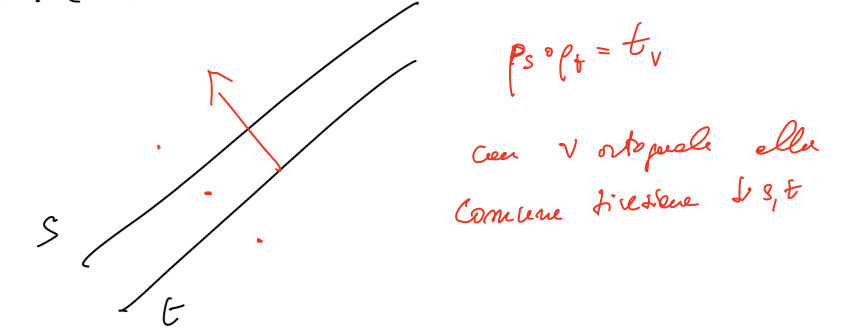
\includegraphics[scale=.4]{rette_parallele.png}\\
In coordinate rispetto ad un riferimetno cartesiano $Oe_1e_2$ Se $P\equiv\icol{x_1\\x_2}$ 
\[
	(R_{C,\theta}\circ R_{D,\varphi})(P) \ \ \ \text{ ha coordinate}
.\] 
\[
	R_\rho(R(x-d) + d-x) + x  
.\]
dove $c,d$ sono i vettori delle coordinate di $C,D $ rispettivamente\\
\begin{aligned}
	&\underline{R_{\theta + \varphi}(x - d)} + R_\theta(d-c) + c\\[-5px]
	&\hspace{-4px}\text{ parte lineare}
\end{aligend}\\[10px]
$T$ T è una translazione se e solo se $\theta + \varphi = 2k\pi, k\in\mathbb{Z}$ e in tal caso
\[
T(x) = x + R_\theta(d-c) = (d-c)
.\] 
che è l'identità se e solo se $d = c$ cioè $D=C$
\begin{defi}[Glissoriflessione]
	Una glissoriflessione è un'isometria di un piano euclideo ottenuta come composizione $t_v\circ\rho_r$ di una riflessione di asse $r$ con una traslazione $t_v\neq Id$ con $v\neq 0, v\parallel r$
\end{defi}
\begin{center}
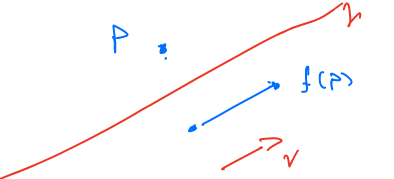
\includegraphics[scale=.4]{glissoriflessione.png}\\
\end{center}
\begin{teo}[Charles, 1831]
	Un'isometria di un piano euclideo che fissa un punto è una rotazione o una riflessione a seconda che sia diretta o inversa. Un'isometria senza punti fissi è una traslazione o una glissoriflessione a seconda che sia diretta o inversa
\end{teo}
\begin{dimo}
	Sia $f\in Isom(E)$\\ Se $f$ ha un punto fisso abbiamo già visto che $f$ è una rotazione se è diretta o una riflessione se $f$ è inversa\\
	se $f$ diretta priva di punti fissi. Allora anche $f^2$ non ha punti fissi, perché se $f^2(p) = p$ \\
	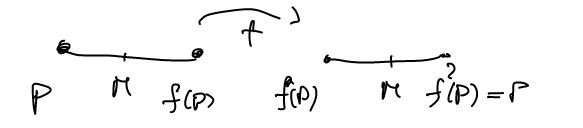
\includegraphics[scale=.4]{f_punti_fissi.png}\\
	Dunque $f(M) = M$ escluso.\\
	DIco che $p,f(p),f^2(p)$ che sono distinti per quanto abbiamo visto, sono allineati, Altrimneti  \\
	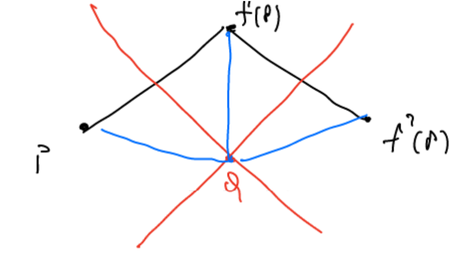
\includegraphics[scale=.6]{batman.png}
	\[
		d(P, f(p)) = d(f(p), f^2(p)) (\text{ poichè } f \text{ è un'isometria})
	.\] 
	\[
		d(Q,P) = d(Q,f(P)) = d(Q,f^2(P))
	.\] 
	Poiché $f$ preserva l'orientazione, il triangolo $QPf(P)$ viene trasformato in  $Q,f(P),f^2(P)$ da cui $f(Q) = Q$\\
	Dunque tutti i punti  $f^i(P), \ \ i\geq 0$ sono allineati, quindi se  $r$ è la retta che li contiene, $f$ agisce su $r$ come una traslazione.\\
	Poiché $f$ è diretta, $f$ agisce su tutto il piano come una traslazione.\\[10px]
	Sia ora $f$ inversa senza punti fissi,\\ Allora $f^2$ è diretta e come prima $f^2= t_v$ per qualche $v$\\
	Sia $P\in E$ un punto $r_0 = \overrightarrow{Pf^2(P)}, \ \ r_1 = \overrightarrow{f(P)f^2(P)}$ \\
	sono rette parallele che sono scambiate tra loro da $f$ \\
	\begin{center} 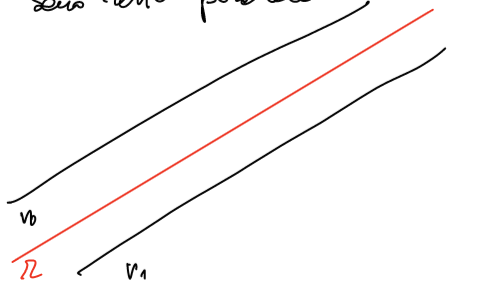
\includegraphics[trim={0 0 0 25px},clip,scale=.4]{rette_scambiate.png}\end{center}\\
	Sia $r$ la retta equidistante da $r_0$ e $r_1$.\\ Allora $f(r)\subseteq r  $ Ma $f^2 = t_v$ 
	$f|_r = t_{v/2}$\\
	Se ora consideriamo $t_{-v/2}\circ f$ \\questa è un'isometria inversa che fissa puntualmente $r$,\\ quindi è una riflessione che indichiamo con $\rho$. Dunque
	\[
		f = t_{v/2}\circ t_{-v/2}\circ f = t_{ v/2}\circ \rho
	.\] 
\end{dimo}
\subsection{Diagonalizzazione di operatori simmetrici}
\textbf{Ricorda}\\
$f\in End(V) $ diagonalizzabile se esiste una base di $V$ di autovettori di  $f\\ \Leftrightarrow A = [f]^B_B$ B base $\exists N\in GL(n,\mathbb{K}): N^{-1}AN$ è diagonale 
\begin{lemm}
	Il polinomio caratteristico di $A\in M_n(\mathbb{R})$ simmetrica ha solo radici reali
\end{lemm}
\begin{dimo}
	$A\in M_n(\mathbb{R}) \subseteq(\mathbb{C}) \ \ L_A : \mathbb{C}^n \rightarrow \C ^n.\\$
	Sia $\lambda\in \C$ un autovalore e $x\neq 0$ un corrispondente autovettore 
	\[
	Ax = \lambda x
	.\] 
	\[
		\overline{Ax} = \overline{\lambda x}
	.\] 
	\[
		A\overline{x} = \overline{\lambda}\overline{x}
	.\] 
	$\overline{x}^tAx = \overline{x}^t(Ax) = \overline{x}^t(\lambda x) = \lambda \overline{x}^t x\\
	\overline{x}^t A x = \overline{x}^t A^t x = (A\overline{x})^tx = (\overline{\lambda}\overline{x})^tx = \overline{\lambda}\overline{x}^tx$\\
	$\overline{x}^tx = \sum^n_{i=1}\overline{x}_ix_i$ $\leftarrow$ è un numero reale positivo poiché $x\neq 0$
	\[
		\lambda \overline{x}^tx = \overline{\lambda}\oveline{x}^tx \ \ \ \Rightarrow \ \ \ \lambda = \oveline{\lambda}
	.\] 
\end{dimo}
\begin{teo}[Teorema Spettrale]
	Sia $V$ uno spazio euclideo di dimensione finita e $T\in End(V)$ un operatore simmetrico, esiste una bas ortonormale di autovettori per $T$
\end{teo}
\begin{coro}
	Per ogni matrice reale simmetrica $A\in M_n(\R)$ esiste una matrice ortogonale $N\in O(n)$ tale che 
	 \[
		 N^{-1}AM = N^tAN \ \ \ \ \ \text{ è ortogonale}
	.\] 
\end{coro}
\begin{dimo}[Teorema]
	 Per induzione su $n = dim(V)$. Base $n = 1$ ovvia\\
	 Supponiamo $n = dim(v) \geq 2$. Poichè $T$ è simmetrico il polinomio caratteristico ha radici reali (per il lemma precedente) quindi $T$ ammette un autovalore $\lambda$ d sia $e_1$ il suo corrispondente autovettore di lunghezza $1$
	 \[
	 V = \R e_1\oplus(\R e_1)^\perp
	 .\] 
	 Chiamo $U \equiv (\R e_1)^\perp$ \\Dico che $T|_U :U \rightarrow$, per cui $T|_U\in End(U)$\\
	 Infatti, dimostro che $u\in U \rightarrow T(u)\in U$\\
\textbf{ipotesi: } $ \langle u, e_1 \rangle = 0$\\
\textbf{Tesi:} $ \langle Tu, e_1 \rangle  = \langle u, T^te_1 \rangle = \langle u, Te_1 \rangle = \langle u, \lambda e_1 \rangle  = \lambda \langle u, e_1 \rangle  = 0$\\
dove abbiamo usato la simmetria di T\\
Chiaramente $T|_U$ è simmetrico, quindi per induzione $U$ ha una base ortonormale di autovettori $\{e_2,\ldots,d_n\}$.\\
Ne segue che $\{e_1,\ldots,e_n\}$ è una base ortonormale di $V$ formata da autovettori per $T$
\end{dimo}
\subsection{Prodotto Hermitiano}
	$V$ spazio vettoriale complesso
	\begin{defi}[Funzione sesquilineare]
		Una funzione sesquilineare su $V$ è un'applicazione $h: V\times V \rightarrow \mathbb{C}$\\
		che è lineare nella prima variabile e antilineare nella seconda, cioè\\[10px]
		\begin{aligned}
			\hspace{80px}&h(v+v',w) = h(v,w) + g(v',w)\\
		&h(\alpha v,w) = \alpha h(v,w)\\
		&h(v,w + w') = h(v,w) + h(v,w')\\
			&h(v,\alpha w) = \overline{\alpha}h(v,w)\\
		\end{aligned}\\[10px]
		per ogni scelta di $v,w,v',w'\in V$ e $\alpha \in\mathbb{C}$
	\end{defi}
	\begin{defi}[Forma hermitiana]
		Una forma sesquilineare si dice hermitiana se
		\[
			h(v,w) = \overline{h(w,v)}
		.\] 
	\end{defi}
	\textbf{Osservazione}\\
	Se $h$ è hermitiana, $h(v,v)\in\R$, infatti deve risultare $h(v,v) = \overline{h(v,v)}$
	\begin{defi}[Forma antihermitiana]
		Una forma sesquilineare si dice antihermitiana se 
		\[
			g(v,w) = - \overline{h(v,w)}
		.\] 
	\end{defi}
	\textbf{Osservazione}\\
	In questo caso $h(v,v)\in\sqrt{1}\R$\\
	\begin{defi}
		Una forma hermitiana si dice semidefinita positiva se 
		\[
		h(v,v) \geq 0 \ \ \forall v\in V
		.\] 
	\end{defi}
	\begin{defi}
		Una forma hermitiana si dice definita positiva se 
		\[
		h(v,v)>0 \ \ \forall v \neq 0
		.\] 
		ovvero
		\[
			(h(v,v)\geq 0 \text{ e }h(v,v) = 0 \Rightarrow v=0)
		.\] 
	\end{defi}
	\textbf{Esempio}\\
	$V = \C^n$
	\[
		h( \icol{z_1\\ \vdots \\ z_n},\icol{w_1\\\vdots\\w_n}) = \sum^n_{i=1}z_i\overline{w_i}
	.\] 
	questo viene chiamato prodotto hermitiano standard su $\C^n$
 \[
		h( \icol{z_1\\ \vdots \\ z_n},\icol{z_1\\\vdots\\z_n}) = \sum^n_{i=1}z_i\overline{z_i} = \sum^n_{i=1}|z_i|^2
	\]
	\newpage
	Dato $V$, consideriamo una base $B = \{v_1,\ldots,v_n\}$ di $V$ Se $h$ è una forma heritiana, diciamo che $(h_{ij}) = h(v_i,v_j)$ è la matrice che rappresenta $h$ nella base $B$ e la denoto come $(h)_B$\\
	se  $v = \sum^n_{i=1}x_iv_i, \ \ \ w = \sum^n_{i=1}y_iv_i$\\
\begin{aligned}
	\hspace{30px}h(v,w) &= h(\sum^n_{i=1}x_iv_i,\sum^n_{i=1}y_iv_i) = \\
&= \sum^n_{i=1}x_ih_i(v_i,\sum^n_{i=1}y_iv_i) = \\
& = \sum^n_{i=1}x_i\overline{y_i}h(v_i,v_i) = \\
& = x^t H\overline{y}
\end{aligned}\\
Poiché $h$ è hermitiana, $h(v,w) = \overline{h(w,v)}$\\
\begin{aligned}
	X^tHY &= \overline{Y^tHX}\\
	 &     = \overline{Y}^t \overline{H} \overline{X}\\
	 & = (\overline{Y}^t \overline{H} \overline{X})^t\\
	 & = \overline{X}^t \overline{H}^t \overline{Y} \ \ \ \ \Rightarrow \ \ \  H = \overline{H}^t
\end{aligned}
\begin{defi}
	Una matrice $M\in M_n(\C)$ si dice hermitiana se
	\[
		H = \overline{H}^t
	.\] 
\end{defi}
\textbf{Esercizio}\\
le matrici hermitiane $2\times 2$ sono un $\R$-sottospazio di $M_2(\C)$ di dimensione 4
\[
	\matrice{a_1 + ib_1 & a_2 + ib_2\\ a_3 + ib_3 & a_4 + ib_4} = \matrice{a_1 - ib_1 & a_3 - ib_3\\a_2 - ib_2 & a_4 - ib_4}
.\] 

$\Rightarrow \hspace{20px}$\begin{aligned}
	& a_1 + ib_1 = a_1 - ib_1 \Rightarrow  b_1 = 0\\
	&a_2 + ib_2 = a_3 - ib_3 \Rightarrow  a_2 = a_3 \ \ b_2 = -b_3\\
	&a_3 + ib_3 = a_2 - ib_2\Rightarrow  a_2 = a_3 \ \ b_2 = -b_3\\
	&a_4 + ib_4 = a_4-ib_4 \Rightarrow b_4 = 0\\[10px]
\end{aligned}\\
\begin{aligend}
	&\matrice{a_1&a_2+ib_2\\a_2-ib_2&a_4}\\[10px]
	&M_2 = \R\icol{1&0\\0&0}\oplus\R\icol{0&0\\0&1}\oplus\R\icol{0&1\\1&0}\oplus\R\icol{0&i\\-i&0}
\end{aligend}\\
\newpage
Si definiscano allo stesso modo del caso reale simmetrico $S^t$\\
coefficiente di Fourier
\[
| \langle v, w \rangle |\leq ||v||||w||
.\] 
disuguaglianza triangolare $||v+w||\leq||v|| + ||w||$\\
Operatore unitario: $T\in End_\C(V)$ t.c.
\[
\langle T(u), T(v) \rangle  = \langle u, v \rangle \ \ \ \forall u,v\in V
.\] 
Verifichiamo le caratteristiche degli operatori unitari dati nel caso reale\\
\textbf{Gram Schmidt}\\
$T\in End(V)$ operatore unitario\\
$1.$ Gli autovalori hanno modulo 1\\
$2.$ Autospazi relativi ad autovalori distinti sono ortogonali\\
$1.$ Sia $v$ un autovettore di autovalore $\lambda$ 
\[
	\langle v, v \rangle = \langle Tv, Tv \rangle  = \langle tv, tv \rangle  = \lambda\overline{\lambda} \langle v, v \rangle = |\lambda|^2 \langle v, v \rangle 
.\] 
\[
v \neq 0 \Rightarrow  \ \ \ |\lambda|^2 = 1 \ \ \  \Rightarrow  \ \ \ |\lambda| = 1
.\] 
$2.$ Sia $v\in V_\lambda$, $w\in V_\mu$ \ \ $\lambda\neq\mu$
\[
	\langle v, w \rangle  = \langle Tv, Tw \rangle = \langle \lambda v, \mu w \rangle = \lambda\overline{\mu} \langle v, w \rangle 
.\] 
Se $ \langle v, w \rangle \neq 0 $ \neq 0 \Rightarrow \lambda \overline{\mu} = 1$. Per il punto 1\\
\[
	\lambda\overline{\lambda} \ \ \Rightarrow \ \ \overline{\lambda} = \overline{\mu} \ \ \Rightarrow \ \ \lambda = \mu \ \ \text{ assurdo}
.\] 
\begin{defi}
	Diciamo che $U\in M_n(\C)$ è unitaria se 
	\[
		U\overline{U}^t = Id
	.\] 
\end{defi}
\begin{prop}
	$T\in End(V)$ è unitario se e solo se la sua matrice in una base ortonormale è unitaria
\end{prop}
\begin{dimo}
	Sia $B = \{v_1,\ldots,v_n\}$ una base ortonormale di $V$ 
	\[
		\delta_{ij} = \langle v_i, v_j \rangle  = \langle Tv_i, Tv_j \rangle  = \langle Ae_i, Ae_j \rangle = e_i^tA^t\overline{A}e_j = A_i^t\overline{A}_j
	\] 
	dove abbiamo posto $A = (T)_B$ e $\{e_i\}$ è una base di $\C^n$\\
	w dove $A_{i}, A_{j}$ sono la $i$-esima e la $j$-esima colonna di $A$\\
	($A_i^t\overline{A}_j$ è il prodotto hermitiano standard)
\end{dimo}\\
Come nel caso reale si dimostra
\begin{teo}
	Sia $T\in End(V)$ un operatore unitario Esiste una base standard di autovettori per $T$
\end{teo} 
In particolare, per ogni matrice unitaria $A\in U(n)$ esiste $M\in U(n)$ tale che $M^{-1}AM$ è diagonale
\begin{nota}
	a volte si pone 
	\[
	 A^* = \overline{A}^t
	.\] 
	$A$ unitario $AA^* = Id$ \\
	$A$ hermitiano $A = A^*$ \\
	$A$ antihermitiano $A=-A^*$
\end{nota}
\begin{defi}[Operatore Aggiunto]
	Dato $T\in End(V)$, esiste unico $S\in End(V)$ tale che 
	\[
	\langle Tu, w \rangle = \langle u, Sw \rangle \ \ \forall u,w\in V
	.\] 
	Tale operatore è detto aggiunto hermitiano di $T$ e denotato con $T^*$
\end{defi}
\begin{defi}[operatore normale]
	Sia $V$ uno spazio vettoriale complesso dotato di prodotto hermitiano (forma hermitiana definita positiva), un operatore $L\in End(V)$ è normale se 
	\[
	L\circ L^* = L^*\circ L
	.\] 
\end{defi}
\textbf{Osservazione}\\
$L$ unitario, hermitiano, antihermitiano $ \Rightarrow$ $L$ diagonale
\begin{teo}
	Sono equivalenti le seguenti affermazioni:\\
	$1)$ $L$ è normale\\
	$2)$ esiste una base ortonormale di $V$ formata da autovettori di $L$
\end{teo}
\newpage
	\subsection{Diangonalizzazione unitaria di operatori normali}
	($\C^n$, prodotto hermitiano standard) $M^\star = \overline{M}^t$\\
	 $M$ è normale se $MM^\star = M^\star M$\\
	 siano normali le matrici\\ \begin{aligned}
		 \hspace{120px}&\text{unitarie} \ \ \ \ &MM^\star = Id\\
						       &\text{hermitiane} \ \ \ \ &M=M^\star\\
						       &\text{antihermitiane} \ \ \ &M = -M^\star
	 \end{aligned}\\
	 \begin{teo}[Spettrale]
	 	$M$ è normale se e solo se $\exists U\in U(n) : \ U^tMU$ è ortogonale
	 \end{teo}
	 \textbf{Nota}\\
	 $U(n)$ spazio delle matrici unitarie\\$
	 \subsection{Classificazioni delle isometrie}
	 \begin{nome}
	$\cdot$ rotazioni\\
	$\cdot$ riflessioni\\
	$\cdot$ traslazioni\\
	$\cdot$ glissoriflessione $ = t_v\circ s_\alpha$ con $v\parallel \alpha^t$ (disegno de li mortacci sua)\\
$\cdot$ glissorotazioni $= t\circ R$ dove $v \parallel a$, $a$ asse di $R$ (altro disegno)\\
$\cdot$ riflessioni rotatorie $s_a\circ R$  $R$ rotazione di asse $\underline{a}$,  $s_\underline{a}$ è una riflessione rispetto ad una retta parallela ad $\underline{a}$
\end{nome}
\begin{teo}[Eulero 1776]
	Ogni isometria di $\mathbb{E}^3$ è di uno dei sei tipi sopra descritti
\end{teo}
\subsection{Teoremi vari su spazi Hermitiani e company}
	\begin{lemm}
		Sia $V$ uno spazio vettoriale su un campo $\R$\\
		Siano  $P,Q\in End(V)$ tali che $PQ=QP$. Allora, se  $V_\lambda$ è l'autospazio di autovalore $\lambda$ su $P$, risulta
		\[
		Q(V_\lambda)\subseteq V_\lambda
		.\] 
	\end{lemm}
	\begin{dimo}
		Sia $v\in V_ \lambda $ (cioè $P(v) = \lambda v)$. Dobbiamo vedere che $Qv\in V_ \lambda$.
		\[
		P(Q(v)) = (P\circ Q)(v) = (Q\circ P)(v) = Q( \lambda v) = \lambda Q(v)
		.\]
	\end{dimo}
	$(V,h)$ spazio Hermitiano (Spazio vettoriale complesso $h$ forma hermitiana definita positiva in $V$ )\\
	$\dim(V) < +\infty$
	 \begin{teo}
		Sia $(V,h)$ uno spazio hermitiano, $L\in End(V)$ operatore, sono equivalenti
		\begin{itemize}
			\item $L$ è normale (rispetto ad $h$)
			\item esiste una base ortonormale $B$ di  $V$ composta da autovettori per $L$
		\end{itemize}
	\end{teo}
	\begin{lemm}
		$(V,h)$ spazio hermitiano, $L\in End(V)$ normale\\
		sono equivalenti
		\begin{itemize}
			\item $Lv = \lambda v$
			\item  $L^\star v = \overline{ \lambda} v$
		\end{itemize}
		In particolare $ \lambda$ è l'autovalore per $L$ se e solo se $\overline{ \lambda}$ è autovalore per $ L^\star$ 
		\[
			V_ \lambda (L) = V_{\overline{ \lambda}}(L^\star)
		.\] 
	\end{lemm}
	\begin{dimo}
		Se $v = 0$ non c'è niente da dimostrare.\\
		Se $v \neq 0$ basta far vedere che se $v\in V_ \lambda (L)$ allora $v\in V_{\overline{ \lambda}}(L^\star)$. L'inclusione contraria segue da $L^{\star t} = L$
		 \[
		w\in V_ \lambda (L), \ \ v\in V_ \lambda (L)
		.\] 
		\begin{aligned}
			\hspace{80px}h(L^\star(v),w) &= h(v,L(w)) = h(v, \lambda w)\\
					&=\overline{ \lambda}h(v,w) = h(\overline{ \lambda}v,w)
		\end{aligned}\\
		\[
			h(L^\star(v) - \overline{ \lambda}v,w) = 0 \ \ \circledast
		\] 
		Per il lemma, siccome per ipotesi $L$ è normale, 
		 \[
		L^\star (v)\in V_\lambda (L), \ \ \overline{
		\lambda}v\in V_ \lambda (L)
		\] 
		\[
			\Rightarrow \ \ \ L^\star (v) - \overline{ \lambda} v\in V_ \lambda (L)
		\] 
		Quindi nella $\circledast$ posso prendere $w = L^\star (v) - \overline{ \lambda} v$, ottenendo 
		\[
			h(L^\star (v) - \overline{ \lambda} v, L^\star (v) - \overline{\lambda} v) = 0
		.\] 
		Poiché $h$ è definito positivo, segue\\
		\begin{aligned}
			&L^\star(v) - \overline{ \lambda}v = 0\\
			\text{cioè} \hspace{50px}  & L^\star (v) = \overline{ \lambda} v
		\end{aligned}\\
	\end{dimo}
	\textbf{Osservazione}\\
	Dal lemma segue $V_ \lambda(L) \perp V_\mu (L)$ se $ \lambda \neq \mu$
	\[
	v\in V_ \lambda, \ \ \ w\in V_\mu
	\] 
	\[
		\lambda h(v,w) = h( \lambda v,w) = h(Lv,w) = h(v,L^\star w) = h(v, \overline{\mu}w) = \mu h(v,w) \Rightarrow  h(v,w) = 0
	\]
	Dato che $ \lambda \neq \mu$
	\begin{dimo}[Teorema Spettrale]
		$1) \Rightarrow  2)$ Procediamo per induzione su $\dim V$,con base ovvia $\dim V = 1$ \\
		Supponiamo il teorema vero per gli spazi hermitiani di dimensione $\leq n-1$ e sia  $\dim_\C V = n$\\
		Sia  $v_1\in V$ un autovettore per $L$, che possiamo assumere di norma  $1$. Sia $V_1 = \C v_1, W = v_1^perp$.\\
		Allora $V = V_1 \oplus W$.\\
		Poiché $V_1$ è $L$-invariante (per costruzione) e $L^\star$-invariante per il lemma precedente, lo stesso accade per  $W$.\\
		Inoltre $L|_W\in End(V)$ è normale.\\
		Per induzione, esiste una base $h|_W$-ortonormale formata da autovettori per $L|_W$, sia $\{v_2,\ldots,v_n\}.$ Allora $\{v_1,\ldots,v_n\}$ è una base $h$-ortonormale di $V$ formata da autovettori per $L$.\\
		$2) \Rightarrow 1)$. Sia $B = \{v_1,\ldots,v_n\}$ una base $h$-ortonormale di autovettori per $L$. Allora\\
		\begin{aligned}
			\hspace{80px}&[L]^B_B = \bigwedge = \matrice{ \lambda_1  &\ldots& 0\\
				 0  & \ddots & 0\\
			 0  &\ldots & \lambda_n}\\
			    &[L^\star]^B_B = \overline{[L]_B^B}^t = \overline{\bigwedge}\\
			    &[L\circ L^\star]^B_B = [L]^B_B[L^\star]^B_B = \bigwedge\overline{\bigwedge}=\overline{\bigwedge}\bigwedge = [L^\star]_B^B[L]^B_B = [L^\star \circ L]_B^B
		 \end{aligned} \\
		 Poiché la mappa $A \rightarrow [A]^B_B$ è un isomorfismo tra
		 $End(V)$ e $M_{nn}(\C)$, segue 
		 \[
		 L\circ L^\star = L^\star \circ L
		 .\] 
		 cioè $L$ è normale
	\end{dimo}
	\textbf{Osservazioni}\\
	1. È essenziale che $h$ sia definita positiva.\\
	\[
	 h(x,y) = x^tH\overline{y} \ \ \ M = \matrice{1&0\\0&-1}
	.\] 
	non è definita positiva $h(\icol{0\\1},\icol{0\\1}) = -1$
	\[
		L_A:\C^2 \rightarrow\C^2 \ \ A = \matrice{0&i\\i & -2}
	.\] 
	Dico che $L_A$ è autoaggiunto, quindi normale\\
	\begin{aligned}
		\hspace{80px}&h(L_AX,Y) = h(X,L_AY)\\
		&(L_AX)^tH\overline{Y} = X^tH\overline{L_AY}\\
		&X^tA^tH\overline{Y} = X^tH\overline{A}\overline{Y} \ \ \forall X,Y\\
		&A^tH = H\overline{A}\\
		&\matrice{0&u\\i&-2}\matrice{1&0\\0&-1} = \matrice{1&0\\0&-1}\matrice{0&-i\\-i&-2}\\
		&\hspace{47px}\matrice{0&-i\\i&2} = \matrice{0&-i\\i&2}
	\end{aligned}\\
	Calcolo il polinomio caratteristico di $A$ 
	\[
		\det\matrice{t& -i\\-i & t + 2} = t(t+2) + 1 = (t+1)^2
	.\] 
		Ma $A\neq \matrice{-1&0\\0&-1}$, in particolare non è diagonalizzabile\\
		2. Vediamo in dettaglio il fatto che $L|_W$ è normale\\
		Ritornando alla dimostrazione del teorema spettrlae, osserviamo che se $W$ è $L$-invariante è anche $L^\star$-invariante.\\
		Infatti, se $V = \bigoplus_\lambda V_ \lambda(L)$ (per esercizio da dimostrare)\\
		\begin{aligend}
			$W &= \bigoplus_ \lambda (V_ \lambda(L)\cap W)$\\
			   &=\bigoplus_ \lambda (V_{\overline{ \lambda}}(L^\star)\cap W)
			
		\end{aligend}\\
		$=> W$ è $L^\star$-invariante\\
		Adesso osservo che $(L|_W)^\star = (L^\star)|_W$\\
		\begin{aligend}
			&(L\left|_{W)}\circ(L\right|_W)^\star = (L|_W)\circ(L^star|_W) = \\
			&(L\circ L^\star)|_W = (L^\star\circ L)|_W = (L^\star|_W) \circ L|_W = (L|_W)^\star\circ L|_W
		\end{aligend}\\
		\subsection{Richiami su spazi vettoriali duali}
		$V$ spazio vettoriale su $\K$ di dimensione finita
		 \[
		V^V = V^\star = Hom(V,\K)
		.\] 
		sia $A\leq V$
		 \[
			 Ann(A) = A^\# = \{f\in V^\star | f(a) = 0 \ \ \forall a \in A\}
		.\] 
		\textbf{Osservazioni}\\
		1) $A^\# $ è un sottospazio\\
		2) $A^{\#\#} = <A>$ \\
		\begin{aligned}
			\hspace{100px}&i:V \rightarrow V^{\star\star}\\
			&v\in V, \ \ f\in V^\star\\
			& i(v)(f) = f(v)
		\end{aligned}\\
	$V,W$ spazi vettoriali di dimensione finita $f\in Hom_\K(V,W)$, $f^\star\in Hom_\K(W^\star,V^\star)$, la trasposta di f è definita con $\phi\in W^\star$\\
	\hspace{40px}$f^\star(\phi) = \phi\circ f \\
	$\text{ }\hspace{100px}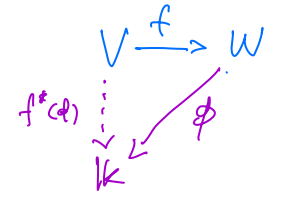
\includegraphics[scale=0.4]{funzione.png}\\
	\newpage
	\begin{defi}
	Definisco la  dualità standard su $V$ come 
	\[
	\langle \ , \  \rangle : V^\star\times V \rightarrow \K
	.\] 
	$\langle v, f \rangle = \langle f, v \rangle = f(v)$\\
	con questa proprietà
	\[
	\langle f(v), w^\star \rangle  = \langle v, f^\star(w^\star) \rangle 
	.\] 
\end{defi}
\hline \ \\
Ricordo che se $B = \{v_1,\ldots,v_n\}$ è una base di $V$ allora i funzionali $v_i^\star$ definiti da
 \[
	 \langle v_i^\star, v_j \rangle =\delta_{ij}
.\] 
per $1\leq i\leq n$ formano una base $B^\star$ di $V^\star$ detta base duale di $B$\\
Sia  $f:V \rightarrow W$ un'applicazione lineare, siano $B =\{v_1,\ldots,v_n\}, L = \{w_1,\ldots,w_m\}$ basi di $V,W$ consideriamo  $f^\star :W^\star \rightarrow V^\star$ Allora:\\
\begin{aligned}
	\hspace{120px}[f&]_B^B = [f^\star]^{B^\star}_{L^\star}^t	\\
		       & \storto{=} \ \ \ \hspace{18px} \storto{=}\\
		       &\hspace{-10px}(a_{ij}) \ \ \ \  (a^\star_{ij})
		        
\end{aligned}\\
\textbf{Tesi} \ \ $a_{ih} = a^\star_{hi}$\\
$f^\star(w^\star_i) = \sum^n_{i=1}a_{ij}^\starv_i^\star$\\
$f^\star(w_i^\star)(v_h) = \sum^n_{i=1}a^\star_{ij}v^\star_i(v_h) = \sum^n_{i=1}a_{ij}^\star\delta_{ih} = a^\star_{hi}$\\
\text{ }\ \ \storto{=}\\
$w_i^\star(f(w_h)) = w^\star_i(\sum^n_{i=1}a_{ih}w_i) = \sum^n_{i=1}a_{ih}w^\star_i(w_i)=$\\
$=\sum^n_{i=1}a_{ih}\delta_{ij}= a_{ih} $
\begin{teo}[Qualche proprietà importante]
	$f:V \rightarrow W$ lineare $\ \ f^\star : W^\star \rightarrow V^\star$\\
	$1) (Im f)^\# = \ker f^\star \\$
	 $2) (\ker f)^\# = Im f^\star$\\
	 $3) (\lambda f + \mu g)^\star = \lambda f^\star + \mu g^\star \ \ \ \ \ \ ( \lambda,\mu \in \K, g\in Hom(V,W)) $\\
	 $4) (h\circ f)^\star = f^\star\circ h^\star \hspace{40px} \ \ \ h:W \Rightarrow U $ lineare
\end{teo}
\begin{dimo}[Il punto 2, 3 e 4 vengono lasciati per esercizio]
	\begin{aligend}
	&1) $\emptyset\in (Im f)^\# $\\
	& \Leftrightarrow \forall w\in Imf \ \ \emptyset(w) = 0 \\
	& \Leftrightarrow \forall v \in V \emptyset(f(v)) = 0\\
	& \Leftrightarrow \emptyset \circ f = 0\\
	& \Leftrightarrow \emptyset \in kerf^\star
	\end{aligend}\\
	Quindi abbiamo visto che $(Imf)^\# = \ker F^\star$
\end{dimo}
\begin{prop}
	Sia $V$ uno spazio vettoriale di dimensione $n$ su $\K$ e $W$ un sottospazio. Allora
	\[
	\dim(W) + \dim W^\#  = n
	.\] 
\end{prop}
\begin{dimo}
	Da quanto visto, la mappa\\
	\begin{aligned}
		\hspace{80px}&Hom(V_1,V_2) \rightarrow Hom(V^star_2,V^star_1)\\
			     & \hspace{20px} \ f \ \ \ \ \ \ \ \  \rightarrow \ \ \  \ \ \ f^t
	\end{aligned}\\
	è un isomorfismo di spazi vettoriali. Inoltre $f$ è iniettiva (rispettivamente suriettiva) se e solo se $f^\star$ è suriettiva (rispettivamente iniettiva)\\
	Consideriamo la proiezione  $\pi:V \rightarrow V|_W :=U$ \\
	Poiché $\pi$ è suriettiva $\pi ^\star : U ^\star \rightarrow V^\star$ è iniettiva e 
	\[
	W^\#  = (\ker\pi)^\# = Im\pi^\star
	.\] 
	per cui 
	\[
	 \dim W^\# = \dim (Im \pi ^\star) = \dim U^\star = \dim V - \dim W
	.\] 
\end{dimo}

	\subsection{Forme bilineari 2}
	$V$ spazio vettoriale su $\R$ \\
	Ricordiamo che una forma bilineare è un'applicazione 
	\[
	b:V\times V \rightarrow \R
	.\] 
	Abbiamo già osservato che se $A = [b]_B$\\
	$X = [v]_B, \ \ Y=[w]_B$
	 \[
	b(v,w) = X^tAY
	.\] 
	Come cambia $[b]_B$ se cambio $B$ \\
	$B = \{v_1,\ldots,v_n\}$ \ \ \  X=[v]_B \ \ X'=[v]_B'\\
	$B' = \{v_1',\ldots,v_n'\}$ \ \ Y = [w]_B \ \ Y' = [w]_B'\\
	$A = [b]_B \ \ A' = [b]_{B'}$\\
	$$b(v,w) = X^tAY = X'^TA'Y'$$
	$X = MX', \ \ Y=MY'\ \ \ M = [Id_V]_B^B$\\
	 \begin{aligend}
		 \hspace{80px} &(MX')^tA(MY') = X'^t A'Y'\\
		 &X'M^t AMY' = X'^tA'Y'\\
		 & \ \ \ A' = M^tAM
	 \end{aligend}\\
\begin{defi}
	Diciamo che due matrici $A,B$ sono congruenti se esiste una matrice invertibile $M$ tale che  $B = M^tAM$
\end{defi}
\begin{prop}
	Due matrici rappresentano la stessa forma bilineare in basi diversi se e solo se sono congruenti
\end{prop}
\textbf{Osservazione}\\
1. La congruenza è una relazione di equivalenza\\
2. Il rango è invariante per la congruenza\\
3. Per matrici reali invertibili, il segno del determinante è invariante\\
4. Se $M$ è ortogonale\\
\[
	M^tAM = M^{-1}AM
.\] 
\hline \ \\
Se ho una forma bilineare $b:V\times V \rightarrow \mathbb{K}$ posso definire due applicazioni $V \rightarrow V^\star$ nel modo seguente.\\
Fissato $v\in V$, \ prendo \ \  \begin{aligned}
	&b_v(w) = b(v,w)\\
	&b_v'(w) = b(w,v)
\end{aligned}\\
È chiaro che $b_v, b'_v\in V^\star$ (usiamo il fatto che $b$ è bilineare)\\
Dunque ho due applicazioni $V \rightarrow V^\star$
\[
\delta_b(v) = b_v  \ \ \ \delta_b '(v) = b'_v
.\] 
\begin{defi}
	Il rango di una funzione bilineare è il rango di una qualsiasi matrice che la rappresenta
\end{defi}
\begin{defi}
	Una forma bilineare è non degenere se ha rango (massimo) $\dim V$
\end{defi}
\newpage
\begin{prop}
Sia $V$ uno spazio vettoriale di dimensione finita,
\[
	b:V\times V \rightarrow \K \text{ una forma bilineare}
.\] 
Sono equivalenti 
\begin{itemize}
	\item $b$ è non degenere ovvero $b(v,v)= 0 \Leftrightarrow v = 0$
	\item $\forall v\in V, v\neq 0\ \ \exists w\in V : \ \ b(v,w)\neq 0$
	\item $\forall w\in V, \ w\neq 0 \ \ \exists v\in V: b(v,w) \neq 0$
	\item $\delta_b :V \rightarrow V^\star$ è un isomorfismo
	\item $\delta_b' : V \rightarrow V^*$ è un isomorfismo
\end{itemize}
\end{prop}
\begin{dimo}
	Sia $B = \{v_1,\ldots,v_n\}$ una base di $V$ e sia $A = [b]_B$\\
	$1) \Rightarrow  2)$ per ipotesi $\det A \neq 0$ se  $X = [v]_B \ \ X\neq 0  \Rightarrow  X^tA\neq 0$ \\
	quindi esiste $Y\in \K^n: X^tAY\neq 0$.\\ Se  $w\in V$ è tale che $[w]_B=Y$ ho dimostrato che  $b(v,w) = X^tAY\neq 0$ \\
	$2) \Rightarrow 1)$ Riscrivendo l'ipotesi in coordinate abbiamo\\
	\begin{aligned}
	\hspace{80px}&\forall X\neq 0 \ \exists Y : \ \ X^tAY\neq 0	\\
	& \Rightarrow X^t A\neq 0 \ \ \forall X\neq 0 \Rightarrow  A \text{ è invertibile}
	\end{aligned}\\
	$1) \Leftrightarrow 3)$ è come sopra\\
	$2) \Rightarrow 4)$ Poiché $\dim V = \dim V^\star$ basta vedere che $\delta_b$ è iniettava, cioè  $\ker\delta_b=\{0\}$\\
	 \begin{aligend}
		&v\in \ker\delta_b \ \ \Rightarrow \ \ \delta_b(v) = b_v \ \text{ è il funzionale nullo, cioè}\\
		&b_v(w) = 0 \ \ \forall w\in V\\
		&b_v(w) = b(v,w) \Rightarrow  v = 0 
	\end{aligend}\\
	$4) \Rightarrow  2)$ Dato $v\neq 0$,  $\delta_b(v) = b_v\neq 0$ perché  $\delta_b$ è un isomorfismo, \\quindi esiste  $w\in V:$\\
	\[b(v,w) = b_v(w)\neq 0\]
	$3) \Leftrightarrow 5)$ è simile a $2) \Leftrightarrow 4)$
\end{dimo}
\subsection{Caso Simmetrico}
\[
b(v,w) = b(w,v)
.\] 
\textbf{Osservazione}\\
$b$ è simmetrica se e solo se lo è qualsiasi matrice che la rappresenta.
\textbf{Dato} $S\subset V$ definiamo
\[
	S^\perp = \{v\in V| b(v,s) = 0 \ \ \forall s\in S\}
.\] 
\textbf{Esercizio} $S^\perp$ è un sottogruppo e, $S^\perp = <s>^\perp$
\begin{defi}
	Due sottospazi $U,W$ si dicono ortogonali se\\
	\[
	Y\subseteq W^perp \ \( \Leftrightarrow W\subset U^\perp )\\\]
\end{defi}
\begin{defi}
	$v\in V$ si dice isotropo se $b(v,v) = 0$\\
\end{defi}
\begin{defi}
	$\ker b = \{ v\in V|b(v,w)=0 \ \ \forall w\in V\} = V^\perp$
\end{defi}
 \textbf{Osservazione}\\
 $b$ è non degenere se e solo se $\ker b = \{0\}$\\
 \begin{prop}
 	Sia $b$ non degenere, $W\subseteq V$ sottospazio,\\
	Allora, se $\delta_b:V \rightarrow V^\star$ è l'isomorfismo canonico indotto da $b$, $\delta_b(W^t) = W^\star.$ In particolare risulta sempre $\dim W + \dim W^\perp = \dim V$
 \end{prop}
 \textbf{Nota}\\
 Non è vero, anche nel caso non degenere, che $V = W\oplus W^\perp$
\begin{dimo}
	$w\in W^\perp\ \ \ \delta_b(w) = b_w$ Voglio vedere che\\
	$b_w\in W^\# \ \ \ b_w(w')=b(w,w')=0 \ \ \forall w'\in W$ \\
	Quindi $\delta_b(W^\perp)\subseteq W^\#$\\
	Prendo ora  $f\in W^\# $; poiché  $b$ è non degenere, $\delta_b$ è un isomorfismo, quindi esiste $v\in V$
	 \[
	f = \delta_b(v) = b_v \ \ b(v,w) = b_v(w) = 0 \ \ \forall w \Rightarrow v\in W^\perp
	.\] 
	quindi $f = \delta(b_v)$ con $v\in W^\perp$
\end{dimo}
\begin{prop}
	Sia $V$ spazio vettoriale, $W\subset V$ sottospazio, $b\in Bi(V).$ Sono equivalenti:
	\begin{itemize}
		\item $V = W\oplus W^\perp$ 
		\item $b|_W$ è non degenere
	\end{itemize}
\end{prop}
\newpage
\begin{lemm}
	$\ker b|_W = W\cap W^\perp$
\end{lemm}
\begin{dimo}[lemma]
	$w\in \ker b|_W \Leftrightarrow b(w,w') = 0 \ \ \forall w'\in W \Leftrightarrow w \in W\cap W'$
\end{dimo}
\begin{dimo}[proposizione]
	$1) \Rightarrow 2)$segue dal lemma perché dall'ipotesi $W\cap W^\perp = \{0\}$ \\
	$2) \Rightarrow  1)$ Sia $\{w_1,\ldots,w_s\}$ una base di $W$ \\
	Per ipotesi $A = (b(w_i,w_j))$ è invertibile, in particolare dato $v\in V$, il sistema lineare
	\[
		* \ \ A\matrice{x_1\\\vdots\\x_s} = \matrice{b(v,w_1)\\\vdots\\b(v,w_s)}
	\]
	ha soluzione unica. Poniamo 
	\[
	w = v - \sum^s_{h=1}x_jw_j
	.\] 
	Notiamo che * significa
	\[
	\sum^s_{h=1}b(v_h,w_j)x_h=b(v,w_j) \ \ 1\leq j \leq s
	.\] 
	Calcoliamo \\
	\begin{aligned}
		&b(w,w_i) = b(v - \sum^s_{h=1}x_hw_h, w_j) =  b(v,w_j) - \sum^s_{h=1}x_hb(w_h,w_j) = b(v,w_j) = \\
		&=b(v,w_i) - b(v,w_i) = 0
	\end{aligned}\\
	Poiché i $\{w_i\}$ sono una base di $W$, risulta $b(w,u) = 0\ \ \ \forall u\in W$, cioè  $w\in W^\perp$ Allora
	\[
	v = w + \sum^s_{h=1}x_hw_h
	.\] 
	Pertanto $V = W + W^\perp$, per ipotesi  $W\cap W^\perp = \ker b|_W = \{0\}$, quindi $V = W\oplus W^\perp$
\end{dimo}
\subsection{Sylvester e forme quadratiche}
\begin{defi}
	 	la forma quadratica associata a $V$ è l'applicazione $q:V \rightarrow \K$ definita da $q(v) = g(v,v)$ e questa è una funzione omogenea di grado $2$
	 \end{defi}
	 \textbf{Esempio}\\
	 $V\cong \K^n, g = $ prodotto scalare standard\\
	 $g\matrice{x_1\\\vdots\\x_n} = \sum^n_{i=1}x_i^2$\\
	 \textbf{Osservazione}\\
	 Valgono:\\
	 1) $q(kv) = k^2q(v)$ \\
	 2) $2g(v,w) = q(v+w) - q(v) - q(w)$\\
	 dove $g(v,w)$ è la forma polare di $q$
	  \begin{dimo}
		  1.\hl{$q(kv)$}$= g(kv,kv) = k^2g(v,v) =$ \hl{$k^2q(v)$}\\
		  2.\hl{$q(v+w)- q(v)-q(w)$} $=g(v+w,v+w) - g(v,v)-g(w,w)= \\
		  =\cancel{g(v,v)}+2g(w,v)+\cancel{g(w,w)}-\cancel{g(v,v)}-\cancel{g(w,w)}= $ \hl{$2g(w,v)$}
	 \end{dimo}
	 \textbf{Osservazione}\\
	 $V=\R^4$ e sia $q\icol{x_1\\x_2\\x_3\\x_4}= x_1^2+2x_2^2-x_4^2+x_1x_4+6x_2x_3-2x_1x_2$\\
	 Voglio trovare la matrice della forma polare di $q$ rispetto  alla base canonica\\
	 $\matrice{1&-1&0&1/2\\-1&2&3&0\\0&3&0&0\\1/2&0&0&-1}$\\
	 Sulla diagonale ci sono i coefficienti delle componenti al quadrato  $(x_i)^2$ gli altri li ottieni dividendo per 2 ogni altro coefficiente 
	\\
	\begin{teo}[(Caratteristica di $\K)\neq 2$]
		Dato $V$ spazio vettoriale di dimensione $n\geq 1$ e  $g$ forma bilineare simmetrica su $V $, allora esiste una base $g$-ortogonale.
	\end{teo}
	\begin{dimo}
		Per induzione su $\dim V = n$. Se  $n=1$ non c'è nulla da dimostrare.\\
		se $g$ è la forma bilineare nulla ($g(v,w)=0 \ \ \forall v,w\in V)$ ogni base è  $g-$ortogonale.\\
		Altrimenti esistono,  $v,w\in V$ con $g(v,w)\neq 0$.\\
		Assumo che almeno uno tra  $v,w,v+w$ è non isotropo. Infatti se $v,w$ sono isotropi
		\[
		g(v+w,v+w)=g(v,v) + g(v,w) + g(w,w) = 2g(v,w)\neq 0)
		.\] 
		quindi $\exists v_1\in V$ t.c $g(v_1,v_1)\neq 0$. Allora $g|_{\K v_1}$ è non degenere quindi $V = \K v_1\oplus W$ con $W = (\K v_1)^\perp$ \\
		$\dim(W) = n-1$, per induzione $\exists$ una base  $\{v_2,\ldots,v_n\}$ di $W$ con $g(v_1,v_j) = 0$ se $2\leq j\leq n, \{v_1,\ldots,v_n\}$ è una base $g$-ortogonale di $V$
	\end{dimo}
	\begin{teo}
		Supponiamo $\K$ algebricamente chiuso. Sia $V$ spazio vettoriale dimensione $n\geq 1$ e $g$ forma bilineare simmetrica su $V$, esiste una base di $V$ rispetto alla quale la matrice di $g$ è $D=\matrice{I_r&0\\0&O_{n-r}}$ r = rg(D)\\
In modo equivalente, ogni matrice simmetrica a coefficienti in  $\K$ è congruente a $D$
	\end{teo}
	\begin{dimo}
		Per il teorema precedente, esiste una base $B´= \{v_1',\ldots,v_n'\}$ di $V$ rispetto alla quale $(g)_{B'}=\matrice{a_{11} &\ldots&0\\
			\vdots & \ddots&\vdots\\
	0&\ldots&a_{nn}}$\\
Possiamo assumere che $a_{11},\ldots,a_{rr}$ siano non nulli e che $a_{r+i,r+i}=0$ con  $1\leq i\leq n-r$.\\
Poiché  $\K$ è algebricamente chiuso, esistono $\alpha_1,\ldots,\alpha_r\in\K$ t.c. $\alpha_i^2= a_{ii}, \ \ 1\leq i\leq r$ poniamo.\\
 $v_i = \begin{cases}
	 \frac {1}{\alpha_i}v_i', \ 1\leq i\leq r\\
	 v_i'\ \ \ \ r+1\leq i\leq n
 \end{cases}$\\
 è chiaro che $\{v_1,\ldots,v_n\}$ è una base. Risulta\\
 $g(v_i,v_i) = \begin{cases}
	 g(\frac{v_i'}{\alpha_i},\frac{v_i'}{\alpha_i} = \farc{1}{\alpha_i^2}g(v_i',v_i') = \frac{a_{ii}}{\alpha_i^2} = 1 \ \ 1\leq i \leq r\\
	 g(v_i',v_i') = 0 \ \ \ \ \ \ \ r+1\leq i\leq n
 \end{cases}$
	\end{dimo}
	\ \\ \textbf{Osservazione}\\
Se $g$ è non degenere, esiste una base  $B$ rispetto alla quale $(g)_B=Id_n$\\
 \textbf{Caso Reale $\K=\R$}\\
$V$ spazio vettoriale reale $(\dim V=n\geq 1)$\\
 $g\in Bi_s(V)$\\
 Sia $B$ una base $g$-ortogonale. Definiamo\\
 \begin{defi}
 	Chiamiamo $i_+(g),i_-(g),i_0(g)$ indice di positività, negatività e nullità di $g$, e sono rispettivamente\\
	\begin{aligend}
		&i_+(g) = \{v\in B|g(v,v)>0\}\\
		&i_-(g) = \{v\in B|g(v,v)<0\}\\
		&i_0(g) = \{v\in B|g(v,v)=0\}
	\end{aligend}
 \end{defi}
 \newpage
 \begin{teo}[Sylvester]
 	Gli indici non dipendono dalla scelta di $B$. Posto $p=i_+(g), q=i_-(g)$ allora $1+q=n-r\ \ \ (r=rg(g))$\\
	ed esiste una base di $V$ rispetto alla quale la matrice $E$ di $g$ è tale che 

	\[
		E = \matrice{Id_p & \ldots & 0\\
			\vdots & -Id_q & \vdots\\
		0 & \ldots & O_{n-r}}
	.\] 
	equivalentemente, ogni matrice simmetrica reale $A$ è congruente ad una matrice della forma $E$ in cui $r = rg(A)$ e $p$ dipende solo da $A$
 \end{teo}
 \begin{dimo}
	 Dal teorema di esistenza di una base $g$-ortogonale deduciamo che esiste una base $\{ f_1,\ldots,f_n\}$ di $V$ rispetto alla quale, se $v = \sum^n_{i=1}y_if_i$\\
	 $q(v) = a_{11}y_1^2 + a_{22}y_2^2+\ldots+a_{nn}y^2_n$\\
	 con esattamente $n$ coefficienti diversi da $0$, che possiamo supporre essere $a_{11},\ldots,a_{rr}$\\
	 Siano $a_{11},\ldots,a_{pp}>0, \ \ a_{p+1,p+1},\ldots,a_{rr}<0$\\
	 $\exists \alpha_1,\ldots, \alpha_p, \alpha_{p+1},\ldots,\alpha_r\in \R$ t.c. \\$\alpha_i^2=a_{ii} \ \ 1\leq i\leq p$  \ \ \  \ $\alpha^2_i  = - a_{ii} \ \ p+1\leq i\leq r$ \\
	 Allora posto $e_i = \begin{cases}
		 \frac{1}{\alpha_i}f_i \ \ 1\leq i\leq r\\
		 f_i \ \ \ r+1\leq i\leq n
	 \end{cases}$\\
	 la matrice di $g$ rispetto a $\{e_1,\ldots,e_n\}$ è $
\matrice{Id_p & \ldots & 0\\
			\vdots & -Id_q & \vdots\\
		0 & \ldots & O_{n-r}}$\\
		Resta da dimostrare che $p$ dipende solo da $g$ e non dalla base $B$ usata per definirlo\\
		Supponiamo che rispetto ad un'altra base $g$-ortogonale $\{b_1,\ldots,b_n\}$, risulti, per $v= \sum^n_{i=1}z_ib_i$ \\
		\[
			q(v)= z_1^2 + \ldots + z_t^2 - z^2_{t+1} - \ldots - z_r^2
		.\] 
		mostriamo che $p=t$\\
	se per assurdo  $p\neq t$ assumo $t\leq p$ considero quindi i sottospazi  $S = < e_1,\ldots,e_n> \ \ T = <b_{t+1},\ldots,b_n>$\\
	Poiché $\dim S+\dim T = p+n-t>n$ perché $t<p$ per Grassman vettoriale $S\cap T\neq \{0\}$ sia $0\neq v\in S\cap T$\\
	allora  $r = x_1e_1+\ldots+x_pe_p = z_{t+1}b_{t+1}+\ldots,z_nb_n$\\
	contraddizione:
	\[
	q(v)= \sum^p_{i=1}x_i^2 >0
	.\] 
	\[
		q(v) =- \sum^r_{i=1}z_i^2 + z_{r+1}^2 + \ldots + z_n^2 <0
	.\] 
 \end{dimo}
	\textbf{Osservazioni}\\
	1. Esiste una definizione più intrinseca degli indici. Ricordiamo che $g\in Bil_S(V), V$ spazio vettoriale su $\R$ è definita positiva se $g(v,v) >0, \ \ \forall v\in V\setminus\{0\}$ e che  $g$ è definita negativa se $-g$ è definita positiva.\\
	2.Il teorema di Sylvester si estende, con la stessa dimostrazione alla forma hermitiana.\\
	In particolare ogni matrice hermitiana è congruente a una matrice diagonale del del tipo
	\[
		\matrice{I_p & \ldots & 0\\
			\vdots & I_{r-p} & \vdots\\
		0 & \ldots & O_{n-r}}
	\] 
\begin{prop}
	Sia $(V,g)$  uno spazio vettoriale su $\R$ dotati di una forma bilineare simmetrica $g$\\
	Siano dati un prodotto scalare $h$ e una forma bilineare simmetrica $k$\\
	Allora esiste una base di  $V$ che sia $h$-ortonormale e $k$-ortogonale
\end{prop}
\begin{dimo}
	$(V,h)$ è uno spazio euclideo, quindi per il teorema di rappresentazione delle forme bilineari, esiste un operatore $L\in End(V)$ tale che
	\[
	h(L(v),w) = k(v,w)
	.\] 
	Poiché $k$ è simmetrica, $L$ è simmetrica, per il teorema spettrale siste una base $h$-ortonormale costituita da autovettori per $L$.\\
	Sia  $\{v_1,\ldots,v_n\}$ tale base. Voglio dimostrare che $\{v_1,\ldots,v_n\}$ è $k$-ortogonale
	\[
		k(v_r,v_s) = h(L(v_r),v_s) = h(\lambda_r v_r,v_s) = \lambda_rh(v_r,v_s) = \lambda_r \delta_{rs}
	.\] 
\end{dimo}
\begin{coro}
	Sia $(V,h)$ uno spazio euclideo, e $k$ una forma bilineare simmetrica  su $V$.\\
	Allora $i_+(k), i_\_(k), i_0(k)$ corrispondono al numero di autovalori positivi, negativi, nulli, dell'endomorfismo di  $V$ che rappresenta $k$ rispetto ad $h$
\end{coro}
\begin{dimo}
	Sia come nella proposizione, $\{v_1,\ldots,v_n\}$ una $h$-ortonormale e $k$-ortogonale, per il teorema di Sylvester
	\[
		i_+(k) = |\{v_i|k(v_i,v_i)> 0\}|
	.\] 
	Ma abbiamo visto che $k(v_i,v_i) = \lambda_i$\\
	quindi $i_+(k) = |\{ \lambda_i>0\}|$.
	La dimostrazione non è terminata.
\end{dimo}
\begin{defi}
	Una matrice simmetrica reale si dice definita positiva se tutti gli autovalori sono positivi
\end{defi}
\begin{defi}
	Data una matrice quadrata $n\times n$, i minori principali leading, sono quelli ottenuti estraendo righe e colonne come segue
	\[
		\{1\},\{1,2\},\{1,2,3\},\ldots,\{1,2,3,\ldots,n\}
	.\] 
\end{defi}
\textbf{Esempio}\\
$ \matrice{1&1&1\\1&-1&0\\1&0&1}$ \\
\begin{aligend}
	&\left|1\right| = 1\\
	&\det\matrice{1&1\\1&-1} = -2\\[5px]
	&\det\matrice{1&1&1\\1&-1&0\\1&0&1} = \det\matrice{1&1\\-1&0} + \det\matrice{1&1\\1&-1} = 1 - 1 - 1 = -1
\end{aligend}
\begin{teo}
	$A$ è definita positiva se e solo se tutti i suoi autovalori principali leading sono positivi
\end{teo}
\end{aligned}
\newpage
\section{Geometria Proiettiva}
\subsection{Spazi proiettivi}
	Servirebbe un'introduzione per tutto ciò, ma non sarà il Posta a darcela, la motivazione matematica è che la formula di Grassmann vale sempre (antani)
	\begin{defi}[Spazio Proiettivo]
		Sia $V$ uno spazio vettoriale di dimensione finita sul campo $\K$. Lo \textbf{spazio proiettivo} associato a  $V$ denominato con $\mathbb{P}(V)$ è l'insieme dei sottospazi $1 $-dimensionali di $V$ \\
		\[
			\K v \leftrightarrow [v] \storto{\storto{\leadsto}} \text{ punto di }\pro(v)
		.\] 
		$\dim V = 0 \ \ \ \mathbb{P}(V) = \emptyset$ \\
		$\dim V = 1 \ \ \ \mathbb{P}(V) = \{pt\}$ \\
		$\dim V = 2 \ \ \ \mathbb{P}(V)$ retta proiettiva\\
		$\dim V = 2 \ \ \ \mathbb{P}(V)$ piano proiettivo\\
		Quindi $\dim \mathbb{P}(V) = \dim V -1$\\
		Caso importante  $V = \K^{n+1}$\\
		 \[
			 \mathbb{P}(V) = \mathbb{P}^n(=\mathbb{P}^n(K))
		.\] 
	\end{defi}
	\textbf{Osservazione}\\
	1. Dati $v\in V\setminus \{0\}, \ \ \ \K v$ è un sottospazio $1 $-dimensionale, quindi esso dà luogo a un punto nello spazio proiettivo che denotiamo $[v]$\\
	2. La nozione di spazio proiettivo di $V$ può introdursi in modo equivalente tramite la seguente relazione d'equivalenza su $V\setminus \{0\}$
	 \[
		 v\sim w \Leftrightarrow \exists \lambda\in \K\setminus\{0\} \text{ t.c. } v= \lambda w
	.\] 
	Allora\\
	\begin{center}
	
\includegraphics[scale=.5]{quoziente.png}\\
	\end{center}
	Riprendendo l'osservazione 1, nel caso $V=\K^{n+1}$
	 \[
		 (x_0,\ldots,x_n)\in\K^{n+1}\setminus\{0\} \leadsto [x_0\ldots,x_n]\in\mathbb{P}^n
	.\] 
	\[
		[x_0,\ldots,x_n]=[y_0,\ldots,y_n]
	.\] 
	\[ \Leftrightarrow\exists \lambda\in\K\setminus\{0\}:\ \ \ y_i= \lambda x_i, \ \ \ 0\leq i\leq n\]\\
	\begin{defi}
		Sia $\mathbb{P}=\mathbb{P}(V)$ ed $\{e_0,\ldots,e_n\}$ una base di $V$.\\
		Diciamo che $\{e_0,\ldots,e_n\}$ definisce un sistema di coordinate omogenee (o riferimento proiettivo) su $V$, denotato con $e_0,\ldots,e_n$
	\end{defi}
	Dato $v\in V\seminus\{0\}$
	 \[
	v= x_0e_0+\ldots +x_ne_n
	.\] 
	$\leadsto (x_0,\ldots,x_n)\in\K^{n+1}\setminus\{0\}$
	\[
		P[x_0,\ldots,x_n] \leftrightarrow P=[v]
	.\] 
	$x_0,\ldots,x_n$ si dicono coordinate omogenee di $v$
\\
Ad esempio, fissata la base $\{e_0,e_1,e_2\}$ in $\mathbb{P}^2$,\\
	$P[1,2,3]$ è il sottospazio $1 $-dim di $V$ generato da $e_0+2e_1+3e_2$\\
	\begin{nome}
		Fissato $e_0\ldots e_n$, i punti 
		\[
			F_0[1,0,\ldots,0] = [e_0],\ldots,F_n[0,\ldots,1]=[e_n] 
		.\] 
\\sono i punti fondamentali del riferimento\\
		$U[1,\ldots,1]$ punto unità del riferimento\\
		\textbf{Nota Bene}\\
		Poichè $[v] = [ \lambda v]$ risulta
		\[
		\lambda v = \lambda x_0e_0+\ldots+ \lambda x_n e_n
		.\] 
		quindi le coordinate omogenee sono determinate solo a meno di un fattore di proporzionalità non nullo
	\end{nome}
	\textbf{Osservazione}\\
	se $e_0,\ldots ,e_n$ è un riferimento proiettivo, anche  $(\mu e_0),\ldots,(\mu e_n), \ \ \mu\in\K\setminus\{0\}$ è un riferimento proiettivo e i punti hanno le stesse coordinate omogenee rispetto ai due riferimenti.\\
	\textbf{Quindi}\\
	consideriamo identici due riferimenti se definiti da basi proporzionali
	\[
	e_0,\ldots,e_n=(\mu e_0),\ldots,(\mu e_n)
	.\] 
	Un riferimento in $\mathbb{P}^n$ determinato dalla base canonica di $\K^{n+1}$ si dice riferimento standard. \\
	i punti fondamentali sono
	\[
		[1,0,\ldots,0],[0,1,\ldots,0],\ldots,[0,\ldots,0,1]
	.\] 
	\hline \ \\
	Dato $W\subset V$ sottospazio vettoriale possiamo considerare $\mathbb{P}(W)\leq \mathbb{P}(V)$\\
	$\mathbb{P}(W)$ è detto sottospazio proiettivo di $\mathbb{P}(V)$
	\[
		\dim\mathbb{P}(V)-\dim\mathbb{P}(W) = (\dim V-1) -(\dim W -1) = \dim V - \dim W
	.\] 

\begin{defi}
	Un iperpiano in $\pro^n$ è un sottospazio proiettivo di codimensione $1$
\end{defi}
Supponiamo che in $\pro^n$ sia fissato un riferimento $e_0,\ldots,e_n$ con coordinate omogenee $x_0,\ldots,x_n$
\[
	\circledast \ \ a_0x_0+a_1x_1+\ldots+a_nx_n=0 \ \ \icol{a_0\\\vdots\\a_n}\neq\icol{0\\\vdots\\0}
.\] 
Se leggiamo quest'equazione in $V$ è l'equazione cartesiana di un iperpiano vettoriale $H\subset V$\\
I punti di  $P=[v]\in \pro$ le cui coordinate omogenee verificano  $\circledast$ sono quelli tali che  $v\in H, \ \ v\neq 0$ quindi sono i punti di  $\pro(H)$ \\
\textbf{Nota bene}\\
Se $[x_0,\ldots, x_n] = [y_0,\ldots,y_n]$ e
\[
a_0x_0+\ldots+ a_nx_n=0
.\] 
allora anche $a_0y_0+\ldots+a_ny_n=0$ perché $[x_0,\ldots,x_n] = [y_0,\ldots,y_n]$ significa $y_i=\mu x_i \ \ \mu\in\K\setminus\{0\}$ e
 \[
a_0y_0+\ldots+a_ny_n=a_0\mu x_0+\ldots+a_n\mu x_n = \mu(a_0x_0+\ldots_a_nx_n)=0
.\] 
\  \hline \ \\
Iperpiani coordinati su $\pro^n$ (rispetto al riferimento standard)\[
	H_i=\{[x_0,\ldots,x_n]\in\pro^n|x_i=0\} \ \ 0\leq i\leq n
.\] 
Ad esempio, in $\pro^2,$   \begin{center}\begin{aligend}
	&H_0=\{x_0=0\}\\
	&H_1=\{x_1=0\}\\
	&H_2=\{x_2=0\}
\end{aligend}\end{center}\\
Più in generale consideriamo un sistema di $t$ equazioni omogenee\\
 \begin{cases}
	 &a_{10}x_0+\ldots a_{1n}x_n=0\\
	 &\ldots\\
	 &a_{t0}x_0+\ldots+a_{tn}x_n=0
 \end{cases}\\
 Se $W\subset V$ è il sottospazio definito dal sistema precedente, l'insieme di punti $P\in \pro$ le cui coordinate verificano il sistema è $\pro(W)$\\
 Sia $A=(a_{ij}) \ \ \ 1\leq i\leq t, 0\leq j\leq n$ e sia  $r=rk(A)$
  $\dim \pro(V)= \dim W -1=\dim V -r - 1 = \dim \pro(V) -r$
  Quindi  $\pro(W)$ ha codimensione $r$ su $\pro$\\
   \textbf{Intersezione}\\
   $A_1x = 0 \ \ \pro(W_1)$\\
   $A_2x=0 \ \ \pro(W_2)$ \\
   \begin{cases}
	&A_1x=0\\
	&A_2x=0
   \end{cases}
   In particolare $\pro(W_1)\cap\pro(W_2)= \emptyset \Leftrightarrow W_1\cap W_2 = \{0\}$
   \begin{defi}
   	$\pro(W_1),\pro(W_2)$ si dicono\\
	Incidenti se $\pro(W_1)\cap\pro(W_2)\neq\emptyset$\\
	Sghembi se $\pro(W_1)\cap\pro(W_2)=\emptyset$
   \end{defi}
   \textbf{Osservazione}\\
   La formula si generalizza in 
   \[
	   \bigcap_{i\in I}\pro(W_i) = \pro\left(\bigcap_{i\in I }W_i\right)
   .\] 
   \begin{defi}
   	Se $\emptyset\neq J\subset \pro$, il sottospazio proiettivo generato da  $J$ è 
	\[
		L(J)=\bigcap_{\pro(W)\supseteq J}\pro(W)
	.\] 
	con $W$ sottospazio di $V$
   \end{defi}
   \textbf{Caso speciale}\\
   $J=\{p_1,\ldots, p_t\}$. Scriveremo in tal caso $L(p_1,\ldots,p_y)$ Notiamo che se
   \[
	   p_1=[v_1],\ldots,p_t=[v_t]
   .\] 
   \[
   L(p_1,\ldots,p_t)=\pro(<v_1,\ldots,v_t>)
   .\] 
   In particolare \\
   $\dim(L(p_1,\ldots,p_t))\leq t-1$ 
   \begin{defi}
   	$p_1,\ldots,p_t$ si dicono linearmente indipendenti se 
	\[
	\dim(L(p_1,\ldots, p_t))=t-1
	.\] 
   \end{defi}
   \textbf{Esempio}\\
   $p_1,p_2$ sono indipendenti $ \Leftrightarrow$ sono distinti \\
   $p_1,p_2,p_3$ sono indipendenti $ \Leftrightarrow$ non sono allineati
   \newpage
   \begin{defi}
   	$p_1,\ldots,p_t$ in $\pro=\pro(V)$, $\dim(V)=n+1$ si dicono in posizione generale se\\
	$\circ$ sono linearmente indipendenti $(t\leq n+1)$\\
	 $\circ$ se $t>n+1$ e $n+1$ tra essi, comunque scelti, sono linearmente indipendenti
   \end{defi}
\textbf{Esempio} su $\pro^2$\\
	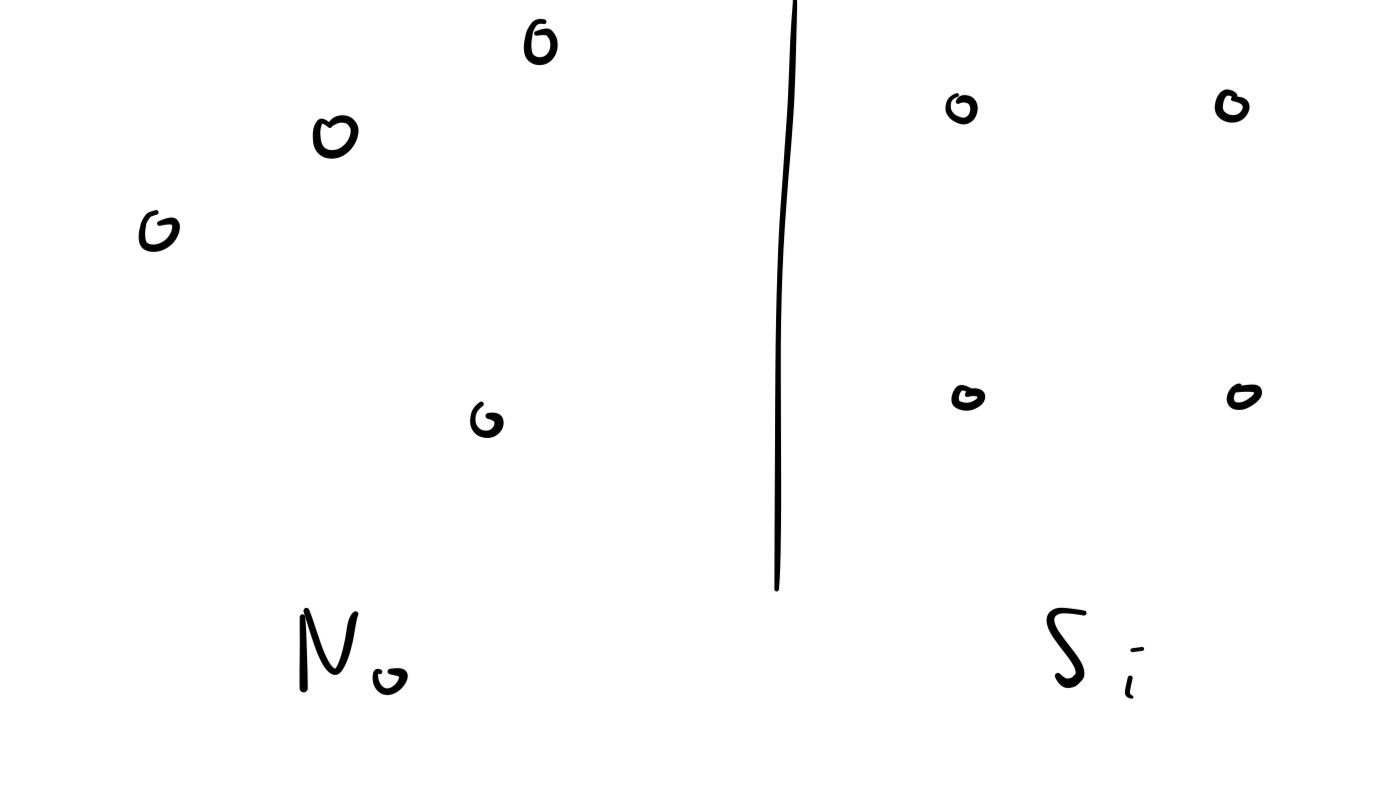
\includegraphics[scale=0.20]{pos_gen.jpeg}
	\subsection{Equazioni parametriche di un sottospazio}
	$k+1$ punti linearmente indipendenti $[v_0],\ldots,[v_n]$ in un sottospazio proiettivo $S$ di dimensione $k$.\\
	Per ogni $P\in S$, 
	\[
		P = [\lambda_0v_0+ \lambda_1v_1+\ldots+ \lambda_k v_k]
	.\] 
	Fissiamo ora un riferimento $e_0,\ldots,e_n$ su $\pro$\\
Allora se $v_i$ ha coordinate $(p_{i0},\ldots,p_{in})^t$ rispetto a $\{e_0,\ldots,e_n\}$ e $P = P[x_0,\ldots,x_n]$ si ha
\begin{center}
\begin{cases}
	x_0 = \lambda_0 p_{00}+ \lambda_1p_{10}+\ldots+ \lambda_k p_{k0}\\
	x_1 = \lambda_0 p_{01}+ \lambda_1p_{11}+\ldots+ \lambda_k p_{k1}\\
	\vdots\\

	x_n = \lambda_0 p_{0n}+ \lambda_1p_{1n}+\ldots+ \lambda_k p_{kn}\\
\end{cases}\end{center}
\textbf{Caso importante}: rette $[v_0],[v_1]$\\
\begin{center}\begin{cases}
	x_0 = \lambda_0 p_{00}+ \lambda_1 p_{10}\\
	x_0 = \lambda_0 p_{01}+ \lambda_1 p_{11}\\
	\vdots\\
	x_0 = \lambda_0 p_{0n}+ \lambda_1 p_{1n}\\
\end{cases}\end{center}\\
\ \\ \hline \ \\
$\pro$ piano proiettivo, $r$ retta per $P[p_0,p_1,2],Q[q_0,q_1,q_2]$ $r$ è un iperpiano in $\pro$ 
\[
	\det\matrice{x_0&x_1&x_2\\p_0&p_1&p_2\\q_0&q_1&q_2}=0
.\] 
\textbf{Esercizio} Se in $\pro^3$ sono dati punti non allineati 
\[
	P[p_0,p_1,p_2,p_3],Q[q_0,q_1,q_2,q_3],R[r_0,r_1,r_2,r_3]
.\] 
l'equazione del piano per $P,Q,E$ è
 \[
	 \det\matrice{x_0&x_1&x_2&x_3\\p_0&p_1&p_2&p_3\\q_0&q_1&q_2&q_3\\r_0&r_1&r_2&r_3}=0
.\] 
\textbf{Esempio} Retta in $\pro^2(\C)$ per $[-1,1,1],[1,3,2i]$
\[
	\det\matrice{x_0&x_1&x_2\\-1&1&1\\1&3&2i}=0
.\] 
$\circ$ Verificare che i punti $A=[1,2,2], B=[3,1,4],C = [2,-1,2]$ di  $\pro^2(\R)$ sono allineati e scrivere un'equazione ella retta che li contiene
\[
	\det\matrice{x_0&x_1&x_2\\1&2&2\\3&1&4}=0
.\] 
$\circ$ Verificare che le rette per $\pro(\C)$ \\
\begin{aligned}
	&ix_1-x_2+3ix_0=0\\
	&x_0+x_1-ix_2=0\\
	&5x_0 + x_1 + 3ix_2=0
\end{aligned}\\
hanno intersezione non vuota (basta verificare che il determinante sia nullo)
\[
	A=\matrice{3i&i&-1\\1&1&-i\\5&1&3i}
.\] 
$\det A = 0$
\ \\ \hline \ \\
Siano $S_1= \pro(W_1), S_2=\pro(W_2)$ due sottospazi proiettivi
\[
	L(S_1\cup S_2) \text{ è detto sottospazio somma}
.\] 
\[
L(S_1,S_2) = P(W_1+W_2)
.\] 
Infatti, se $\pro(W)\supset S_1\cup S_2$, allora contiene $\pro(W_1+W_2)$ perché $W$ deve contenere sia $W_1$ che $W_2$ \\
D'altra parte, $W_1+W_2\supseteq W_1, \ \ W_1+W_2\supseteq W_2$\\
quindi$
\begin{aligend}
	\hspace{20px}&\pro(W_1+W_2)\supseteq P(W_1)=S_1\\
	&\pro(W_1+W_2)\supseteq P(W_2)=S_2
\end{aligend} 
\Rightarrow \supseteq L(S_1,S_2)$
\begin{teo}[Forumla di Grassmann proiettiva]
\[
\dim L(S_1,S_2)=\dim S_1+\dim S_2 - \dim S_1\cap S_2
.\] 
($S1,S_2$ sottospazi proiettivi di $\pro(V)$
\end{teo}
\begin{dimo}
	La dimostrazione segue subito dalla formula di Grassmann vettoriale
	\[
	\dim(W_1+W_2) = \dim W_1 + \dim W_2 - \dim W_1\cap W_2
	.\] 
	$\dim L(S_1,S_2) - 1 = \dim S + 1 + \dim S_2 + 1 - (\dim S1\cap S_2 + 2)$
\end{dimo}
\textbf{Osservazione}\\
Poiché $\dim L(S_1,S_2)\leq \dim \pro$, risulta dalla formula di Grassmann
\[
	\dim S_1\cap S_2 \geq \dim S_1 + \dim S_2 - \dim \pro
.\] 
In particolare
\[
	\dim S_1 + \dim S_2 \geq \dim \pro \Rightarrow S_1,S_2 \text{ sono incidenti}
.\] 
(Infatti $\dim S_1\cap S_2\geq 0 \Leftrightarrow S_1\geq S_2 \neq \emptyset)$ 
\begin{coro}
	1. In un piano proiettivo due rette si intersecano\\
	2. In uno spazio proiettivo di dimensione 3 una retta e un piano si intersecano e due piani distinti si intersecano in una retta
\end{coro}
\subsection{Mappe tra spazi proiettivi}
		Siano $V,W$ $\K$-spazi vettoriali
	\begin{defi}
		Un'applicazione $f:\pro(V) \rightarrow\pro(W)$ si dice trasformazione proiettiva se esiste un'applicazione lineare iniettiva $\varphi : V \rightarrow W$ tale che 
		\[
			f([v])=[ \varphi(v)] \ \ \ \forall \ v  \in V\setminus\{0\}
		.\] 
	\end{defi}
	\textbf{Osservazione}\\
	Scriviamo $f = \bar{\varphi}$ e diciamo che $\varphi$ induce $f$.\\
	Notiamo che $\bar{\varphi} = \overline{ \lambda \varphi} \ \ \ \ \lambda\in \R\setminus\{0\}$ quindi la famiglia $\{ \lambda \varphi | \lambda\in \K\setminus\{0\}$ induce la stessa trasformazione proiettiva
	\begin{nome}
		$\circ$ Se $\varphi$ è un isomorfismo $f=\bar \varphi$ si chiama isomorfismo proiettivo\\
		$\circ$ Se $\varphi : V \rightarrow V$ è un isomorfismo, $f=\bar \varphi$ si chiama proiettività\\
		$\circ$ $A,B\subseteq\pro(V)$ sono proiettivamente equivalenti se esiste proettività $f$ tale che $f(A)=B$
	\end{nome}
	\textbf{Formula di Grassmann Proiettiva}\\
	$S_1 = \pro(W_1) \ \ S_2 = \pro(W_2)$\\
	$S_1\cap S_2=\pro(W_1\cap W_2)$ $\ \ \ L(S_1,S_2) = \pro(W_1+W_2)$\\
	Dove $L(S_1,S_2)$ è il minimo sottospazio che contiene $S_1,S_2$\\
	\[
	\dim L(S_1,S_2) = \dim S_1 + \dim S_2 - \dim (S_1\cap S_2)
	.\] 
	\[
	\Rightarrow \dim(S_1\cap S_2) \geq \dim S_1 + \dim S_2 - \dim\pro
	.\] 
	$ \Rightarrow$  se $\dim S_1 + \dim S_2\geq \dim \pro$ allora $S_1,S_2$ sono incidenti
	\subsection{Sottospazi in posizione Generale}
	\begin{defi}
		$S_1, S_2$ sottospazi di $\pro(V)$ sono in posizione generale se $S_1\cap S_2$ ha dimensione minima
	\end{defi}
	\textbf{Osservazione}\\
	Se $\dim S_1 = h, \dim S_2 = k, \dim\pro =n$ allora $S_1,S_2$ sono in posizione generale se 
	\[
		\dim S_1\cap S_2 = h + k - n \ \ \ \ \text{se } h+k\geq n
	.\]\[
	S_1\cap S_2 = \emptyset \ \ \ \ \ \ \ \text{se } h + k <n
.\]
\begin{defi}[Cono proiettivo]
$J\subseteq\pro(V), \ \ P\in \pro$\\
Il Cono proiettivo  $J$ di $p$ è definito con 
\[
	C_p(J) = \bigcup_{Q\in J}L(P,Q)
.\] 
\end{defi}
\begin{center}
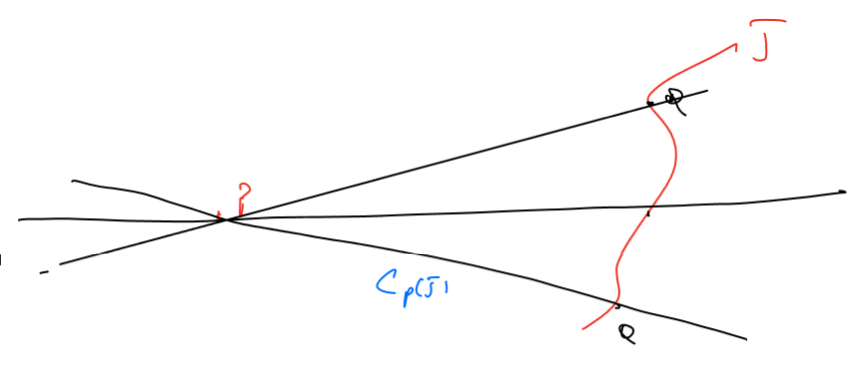
\includegraphics[scale=.53]{cono_proiettivo.png}\\
\end{center}
\textbf{Esercizio}\\
1. $S\subseteq\pro$ è un sottospazio proiettivo, allora 
\[
 C_p(S) = L(P,S) 
.\] 
2. $S_1, S_2$ sono sottospazi proiettivi, allora 
\[
	L(S_1,S_2) = \bigcup_{P_1\in S_1, P_2\in S_2} L(P_1,P_2) = \bigcup_{P_2\in S_2} C_{P_2}(S_1)
.\] 
\ \\ \hline \ \\
$H\in \pro$ iperpiano $P\in \pro\setminus H$\\
La proiezione di  $H$ di centro $P$ è l'applicazione
\[
	\pi_{P,H}:\pro\setminus\{P\} \rightarrow H
.\] 
\[
	\pi_{P,H}(Q) = L(P,Q) \cap H
.\] 
Osserviamo che se $J\subseteq \pro$ e $p\notin J$
 \[
	 \pi_{P,H}(J) = H\cap C_P(J)
.\] 
\textbf{Esempio}\\
$\pro^N, \ \ \ H_0 = \{x_0=0\} = \{[0,x_1,\ldots,x_N]\in \pro^N\}$\\
Dato che punti proporzionali ci danno lo stesso risultato dire $x_0 = 1$ non avrebbe senso, sarebbe identico a $x_0=3$\\[10px]
Se $P = [1,0,\ldots,0]\notin H_0$\\
Se $Q = [x_0,\ldots,x_N]$, allora
\[
	\pi_{P,H}(Q) = [0,x_1,\ldots,x_N]
.\] 
$L(P,Q) = [ \lambda + \mu x_0, \mu x_1,\ldots, \mu x_n]\\$
$L(P,Q)\cap H_0$\\
\textbf{Esempio}\\
$[1,2,1] [0,1,-1]$\\
\[
	\{ \lambda [1,2,1] + \mu [0,1,-1] | ( \lambda,\mu)\in \K^2 \neq(0,0)\}
.\] 
Qui c'è lo spazio quoziente $( \lambda,\mu) / \lambda \sim \mu $
\ \\ \hline \ \\ 
\subsection{Posizione generale di sottospazi in $\pro^3, \pro^4}$}
 \begin{aligned}
	&\dim S_1 = h\\
	&\dim S_2 = k\\
	&\dim \pro = n 
 \end{aligned}\ \ \ $\dim S_1\cap S_2$ = \begin{cases}
	&h + k - n \ \ \ h + k\geq n\\
	&-1 \ \ \  \ \ \ \ \ \ \ \ h + k < n\\
 \end{cases}\\
 \begin{center}
 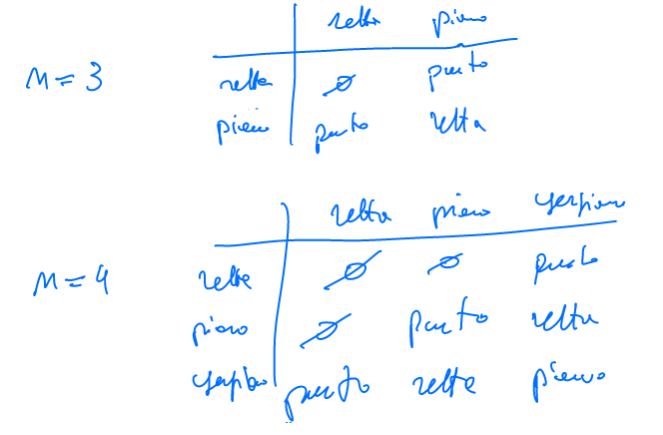
\includegraphics[scale=.5]{tabelle.png}\\
 \end{center}
 \ \\ \hline \ \\
 Osserviamo che in un riferimento proiettivo in $\pro^n$ sia  $e_0,\ldots,e_n$ individua i punti fondamentali ed il punto unità, e questi sono in posizione generale
 \[
	 F_0 = [e_0], \ldots, F_n=[e_n], u  = [e_0 + \ldots + e_n]
 .\] 
 ogni $(n+1)$-ple di righe ha rango massimo
 \begin{aligned}
	& 1 \ \ 0 \ldots \ \ 0\\
	&\dots \ \ \ldots\\
	&0\ \  0 \ldots \ \ 1\\
	&1 \ \ 1\ldots \ \ 1
 \end{aligned}\\
 \textbf{Esempio} $\pro^2$ $[e_0]\ \ \ \ $ \begin{aligned}
	&1 \ 0 \ 0 \\
	&0\ 1 \ 0 \\
	& 0 \ 0 \ 1\\
	&1 \ 1 \ 1
 \end{aligned} $\ \ \ $
 tutti i minori di rango 3 sono non zero\\
 Viceversa, data una $(n+2)$-pla di punti in posizione generale, esiste un unico riferimento proiettivo che il ammette come punti fondamentali e punti unità.\\
 Siano dati $P_0,\ldots,P_n$ n punti in posizione generale, \\supponiamo che $P_i= [v_i] , \ \ i= 0,\ldots,n$\\
 Allora $\{v_0,\ldots,v_n\}$ è una base di $V$. Se $n\in V$ è tale che  $N = [n]$, allora
  \[
 n = \lambda_0v_0+\ldots+ \lambda_n v_n
 .\] 
 in modo unico. \\Osserviamo che per l'ipotesi di posizione generale, tutti i $ \lambda_i$ sono diversi da zero.\\
 Allora $( \lambda_0v_0)\ldots ( \lambda v_n)$ è un riferimento con le proprietà valide: infatti i punti fondamentali sono 
 \[
	 [ \lambda_i v_i] = [v_i] = P_i
 .\] 
 \[
	 [( \lambda_0 v_0) + \ldots +( \lambda_n v_n)] = [n] = V
 .\] 
 \subsection{Esercizi}
 Verificare che in $\pro^2(\R)$
  \[
	  [\frac{1}{2},1,1],\ \ [1,\frac 4 3, \frac 4 3],\ \ [2,-1,2]
 .\] 
 Sono allineati e trovare un'equazione della retta che li contiene\\
 \textbf{Svolgimento}\\[10px]
\begin{agliend}
	0=\det\matrice{x_0&x_1&x_2\\1&2&2\\3&1&4} = 6 x_0 + 2 x_1 - 5x_2 = 12 -2 -10 = 0
\end{agliend}\\
\textbf{Altro Esercizio:}\\
Determinare i valori di $a\in \C$ per cui le rette in  $\pro^2(\C)$
 \[
ax_1 - x_2 + 3ix_0 =0
.\] 
\[
-iax_1 + x_1 - ix_2 = 0
.\] 
\[
3ix_2 + 3x_0 + x_1 = 0
.\] 
sono concorrenti (si intersecano in un punto)\\
\textbf{Svolgimento}\\
Le rette sono concorrenti se e solo se il sistema delle tre equazioni ha una soluzione non nulla
\[
	A = \matrice{3i&a&-1\\-ia&1&-i\\5&1&3i}
.\] 
$\displaystyle\det A  = 0\ \ \ \ ra^2 + 4ia + 7 = 0 \ \ \Rightarrow  \ \ a = \frac{-2 \pm \sqrt{-ra^2-21a^2}}{3} = $ \begin{cases}
	i\\
	-\frac{7}{3}i
\end{cases}\\
\textbf{Altro altro esercizio}\\
Si considerano i punti seguenti in $\pro^3(R)$
 \[
	 P_1 = [1,0,1,2], \ P_2 = [0,1,1,1], \ P_3 = [2,1,2,2], \ P_4=[1,1,2,3]
.\] 
a. Dire se $P_1,P_2,P_3,P_4$ sono in posizione generale\\
b. Calcola $\dim L(P_1,P_2,P_3,P_4$ e trovare equazioni cartesiane\\
c. Completare, se possibile, $P_1,P_2,P_3$ a un riferimento proiettivo di $\pro^3(\R)$\\
 \textbf{Svolgimento}\\
 I punti dati sono in posizione generale se posto $P_i = [v_i]$,  $v_1,v_2,v_3,v_4$ sono linearmente indipendenti
 \[
	 \det\matrice{1&0&1&2\\0&1&1&1\\2&1&2&2\\1&1&2&3}=0
 .\] 
	 Tuttavia il determinante del minore $\matrice{1&0&1\\0&1&1\\0&1&2}$ è diverso da 0 
	  \[
	 L(P_1,P_2,P_3,P_4) = L(P_1,P_2,P_3)
	 .\] 
	 \[
		 \det\matrice{x_0&x_1&x_2&x_3\\1&0&1&2\\0&1&1&1\\2&1&2&2} = 0 \ \ \ \Rightarrow  \ \ -x_0 -2x_1+3x_2-x_3=0
	 .\] 
	 Ultimo punto dell'esercizio\\
	 Per prima cosa si completa ad una base, si può completare con $\icol{0\\0\\0\\1}$ e il determinate è diverso da 0, a questo punto possiamo prendere  $P_1,P_2,P_3$ come prima, $\widetilde{P}^4 = [0,0,0,1] $  $ U = [3,2,4,6]$
\subsection{Significato geometrico geometria proiettiva}
	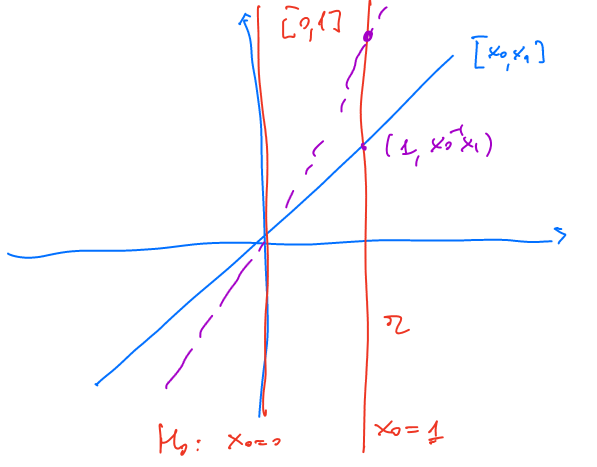
\includegraphics[scale=0.5]{geometria_proiettiva.png}\\
	$\pro^1(\R)=$ rette passanti per $O$  $[x_0,x_1]\in\pro^1(\R)\ \ (\lambda x_0,\lambda x_1)\in\A^2,\ \ \lambda\in\R$\\
	Osserviamo che ogni punto $[x_0,x_1]\in\pro^1\setminus\{H_0\}$ individua una retata parallela ad $r$ (in $\A^2$), che interseca $r$ nell'unico punti $(1,x_0^{-1}x_1)$\\
	(Infatti dobbiamo imporre che $(\lambda x_0,\lambda x_1)$ abbia prima coordinata $1$, cioè $\lambda x_0 = 1$ cioè $\lambda = x_0^{-1}$\\
	Viceversa ogni punto $(1.x)\in r$ appartiene ad un'unica retta per l'origine, quella che corrisponde al punti $[1,x]\in\pro^1\setminus H_0$\\
	In definitiva, abbiamo una corrispondenza biunivoca\\
	\begin{aligned}
		&\pro^1\setminus H_0 \leftrightarrow r\\
		&\pro^1 \leftrightarrow r\cup \{\infty\}\\
		& H_0 \leftarrow \infty \text{ punto all'infinito di } r
	\end{aligned}\\
	La costruzione si generalizza a $\pro^n \leftrightarrow$ rette per l'origine di $\A^{n+1}$\\
	$[x_0,\ldots,x_n]\in\pro^n \leftrightarrow $ rette $\{\lambdax_0,\ldots,\lambda x_{n+1} | \lambda\in \R\}\subseteq \A^{n+1}\ \ \ H_0=\{x_0=0\}$\\
	Consideriamo l'iperpiano affine $A:\{x_0=1\} = \{(1,y_1,\ldots,y_n)\in \A^{n+1}\}$\\
	\begin{center}
	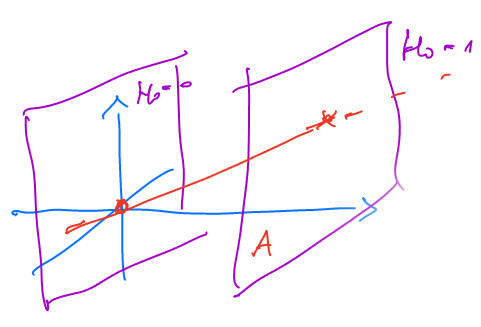
\includegraphics[scale=.5]{Iperpiano_affine_A.jpg}\\
	\end{center}
	\begin{aligned}
		&j: A \rightarrow \pro^n\setminus \{H_0\}\\
		&(1,y_1,\ldots,y_n) \rightarrow [1,y_1,\ldots,y_n]\\
		&y^-1([x_0,\ldots,x_n] = \left[1,\frac {x_1 }{x_0},\ldots, \frac {x_n }{x_0}\right]
	\end{aligned}\\
	Quindi come sopra, ho una corrispondenza biunivoca
	\[
		A\cup \{H_0\} \rightarrow \pro^n
	.\] 
	Se nella costruzione precedente identificavamo $A$ con $\A^n$ tramite  $(1,y_1,\ldots,y_n) \rightarrow (y_1,\ldots,y_n)$ otteniamo\\
	\begin{aligned}
		&j_0:\A^n \rightarrow\pro^n\seminus\{H_0\}\\
		&j_0(y_1,\ldots,y_n) = [1,y_1,\ldots,y_n] \text{ passaggio a coordinate omogenee rispetto a } x_0\\
		&j_0^{-1}([x_0,\ldots,x_n]) = \left(\frac {x_1}{x_0},\ldots,\frac{x_n}{x_0}\right) \text{ passaggio a coordinate non omogenee rispetto ad } x_0
	\end{aligned}|\\
	ci sono analoghe mappe per ogni $i \ \ 0\leq i \leq n$\\
	\ \\ \hline \ \\
	Modello di  $\pro^1 (\C)$ \\
	$E^3$ spazio euclideo con coordinate $x,y,z$ \\
	\begin{aligned}
		&\pi=\{z=0\} \ \ S^2 = \{(x,y,z)\in E^3|d (\icol{x\\y\\0},\icol{0\\0\\0})=1\}\\
		& N = \icol{0\\0\\1}
	\end{aligned}
	\subsection{Proiezione stereografica}
	\begin{center}
	\includegraphics[scale=.3]{Proiezione_stereografica.jpg}\\
	\end{center}
	Se $P = \matrice{x'\\y'\\z'}$\\
	 $\overrightarrow{NP}\ \ \begin{cases}
	 	x = x't\\
		t = y't\\
		z = (z-1)t + 1
	 \end{cases}$\\
	 \sigma \matrice{x'\\y'\\z'} = \matrice{\frac{x'}{1-z'}\\\frac{y'}{1-z'}\\0}\\
	 \textbf{Esercizio}\\
	 $\sigma$ è invertibile con inversa\\
	 \sigma^-1\icol{u\\v\\0}=\matrice{\frac{2u}{u^2+v^2+1}\\\frac{2v}{u^2+v^2+1}\\\frac{u^2+v^2-1}{u^2+v^2+1}}
	 $S^2 \leftrightarrow \pi\cup \{\infty\}$\\
	 identifichiamo  $\pi$ con $\C$ tramite\\
	 \begin{aligend}
		&\pi \ \ \ \ \rightarrow\ \ \ \ \ \C\\
		&\matrice{u&v&0} \rightarrow u + iv
	 \end{aligend}\\
	 Allora abbiamo ottenuto una corrispondenza biunivoca 
	 \[
		 \sigma : S^2 \rightarrow \pro^1{\C} = \C\cup\{\infty\}
	 .\] 
	 \[
	 \sigma(N) =\infty
	 .\] 
	 \[
	 \sigma\matrice{x'\\y'\\z'} = \frac{x'+iy' }{1-z'} \ \ (z\neq 1)
	 .\] 
	 \newpage
	\subsection{Alcuni degli esercizi svolti a lezione}
	 \textbf{Esercizio}\\
	 Determinare un'equazione cartesiana del piano da $\pro^3(\R)$ passante per  $[1,1,0,1]$ e per i punti impropri delle rette
	 \[
	 r = \begin{cases}
	 	x + y + z-1=0\\
		2x-y-z=0
	 \end{cases}
	 .\] 
	 \[
	 s = \begin{cases}
	 	2x-y-2x+1=0\\
		y+z-1=0
	 \end{cases}
	 .\] 
	 Il punto improprio di $r$ è \begin{cases}
	 	x_1+x_2+x_3-x_0=0\\
		2x_1-x_2-x_3=0\\
		x_0=0
	 \end{cases}\\
	 \begin{aligend}
		& \begin{cases}
			x_1+x_2+x_3=1\\
			3x_1-x_2_x_3=0\\
			x_0=0
		\end{cases}
		\Rightarrow \begin{cases}
			x_1+x_2+x_3=0\\
			3x_1=0\\
			x_0=0\\
		\end{cases}
		\Rightarrow \begin{cases}
			x_0=0\\
			x_1=0\\
			x_2+x_3=0
		\end{cases}
		\Rightarrow  [0,0,-1,-1]\\
		&\text{Per quanto  riguarda s}\\
		& \begin{cases}
			2x_1-x_2-2x_3+x_0=0\\
			x_2+x_3-x_0=0\\
			x_0=0
		\end{cases} \Rightarrow  \begin{cases}
			2x_1-x_2-2x_3=0\\x_2+x_3=0\\
			x_0=0
		\end{cases} \Rightarrow \begin{cases}
			2x_1-x_3=0\\
			x_2+x_3=0\\
			x_0=0
		\end{cases} \\&\Rightarrow  [0,1,-2,2]\\
		&\det\matrice{x_0&x_1&x_2&x_3\\1&1&0&1\\0&0&1&-1\\0&1&-2&2}\\
	&\det\matrice{x_0&x_1&x_2&x_3\\1&1&0&1\\0&0&1&-1\\0&1&0&0}\\
	&\det\matrice{x_0&x_2&x_3\\1&0&1\\0&1&-1}=0
	 \end{aligend}
	 \newpage
	 \subsection{Dualità}
	 $\pro^V=\pro(V^\star)\ \ \dim\pro=\dim\pro^V$ poichè  $\dim V=\dim V^\star$\\
	 Osserviamo che  $F,F'\in V^\star$ definiscono lo stesso punto in  $\pro^V$ se e solo se  \\$F'= \lambda F\ \ \ \ \lambda\in\K\setminus\{0\}$\\
	 Ma in questo caso $\ker F = \ker F'$\\
	 Ne segue che l'iperpiano  $\ker F$ dipende solo da  $[F]$ Quindi si ha un'applicazione di dualità 
	  \[
		  \delta :\pro^V \rightarrow \{\text{iperpiani di }\pro\}
	 .\] 
	 \[
		 \delta([F]) = \pro(\ker F)
	 .\] 
	 \textbf{$\delta$ è biunivoca}\\
	 è iniettiva perché due funzionali non nulli che hanno lo stesso nucleo sono proporzionali.\\
	 Inoltre l'iperpiano di $V$ è il nucleo di un funzionale, quindi  $\delta$ è suriettiva\\
	 \ \hline \ \\
	 Diciamo che gli iperpiani $H_1,\ldots,H_s$ in $\pro$ sono linearmenete indipendenti se lo sono $\delta^{-1}(H_1),\ldots,\delta^{-1}(H_s)$ \ \\ \hline \ \\
	 Sia $\{e_0,\ldots,e_n\}$ una base di $V$ e sia $\{\eta_0,\ldots,\eta_n\}$ la corrispondente base duale di $V^\star:\eta_i(e_i)=\delta_{e_i}$ 
	 \[
	 H\subseteq \pro^n \ \ a_0x_0+\ldots+a_nx_n=0
	 .\] 
\[
	H = \pro(\ker F) \ \ F\in V^\star \text{ definita :}
\] 
\[
F(\sum^n_{i=1}x_ie_i)=\sum^n_{i=1}a_ix_i
.\] 
Dove le $a_i$ sono le coordinate omogenee di  $[F] $ rispetto al riferimento proiettivo  $\{\eta_0,\ldots,\eta_n\}$\\
In particolare $H=\delta([F]) \ \ \ H=H[a_0,\ldots,a_n]$ \\
\begin{aligend}
	&H_0=H_0[1,\underline{0},\ldots,\underline{0}]=\delta([\eta_0]\\
	&\vdots\\
	&H_n=H_n[0,\ldots,0,1]=\delta([\eta_n])
\end{aligend}
\begin{defi}
	$S\subset \pro$ sottospazio,  $\dim S = k \leq n-1$
	\[
		\bigwedge_1(S) = \{\text{ iperpiani di }\pro \text{ che contengono } S\}
	.\] 
	dove $\bigwedge_1(S)$ è il sistema lineare di iperpiani di centro $S$
\end{defi}
\textbf{Esempi}\\
$\pro=\pro^2 \ \ S = \{Q\}\ \ \\
\bigwedge_1(Q) = \{$ iperpiani di $\pro^2$  che contengono $Q\}$ = fascio di rette di centro $Q$\\
$\pro=\pro^3 \ \ S = \{r\}\ \ \\ \bigwedge_1(r) = \{$ iperpiani di $\pro^3$ che contengono $r\}$ = fascio di rette di centro $r$\\
$\pro=\pro^3 \ \ S = \{Q\}\ \ \\ \bigwedge_1(Q) = \{$ iperpiani di $\pro^3$ che contengono $Q$\} = stella di rette di centro $Q$\\
\subsection{Parte da rifare seguendo il Sernesi}
	$V$ spazio vettoriale, $V^\star$, \ \ $\pro^V=\pro(V^\star)$ spazio proiettivo duale \\
	Se $B$ è una base di $V$ (ottenuta ad esempio a partire da un riferimento proiettivo di $\pro = \pro(V)$), la base duale  $B^\star$ di $V^*$ può essere usata per introdurre in $\pro^V$ un sistema di coordinate omogenee "duali"
	\[
		0\neq L\in V^\star \ \ [L]\in\pro^V 
	.\] 
	se $x_1,\ldots,x_n$ sono coordinate in $V$ rispetto a $B=\{v_1,\ldots,v_n\}$ 
	\[
	L(x_1v_1+\ldots+x_nv_n) = a_0x_0+\ldots+a_nx_n
	.\] 
	e $L$ ha coordinate $(a_0,\ldots,a_n)$ rispetto alla base $B^\star=\{v_1^*,\ldots,v_n^*\}\ \ \\ (v_i^*(v_j)=\delta_{ij})$\\
\textbf{Questa Lezione è venuta una merda, non c'è modo apparente di studiare questo argomento se non quello di leggerlo dal Sernesi}\\Qui il professore prende letteralmenete un altro file e iniza a scriverci sotto, non sappiamo a cosa si stia riferendo}\\
	Sia $S=\pro(W)$ un sottospazio proiettivo di  $\pro$ di dimensione $k$.
	\[
		W^\# =\{F\in V^*|F|_W=0\}
	.\] 
	$\dim W = n - k$
	\[
		\delta:\{\text{s.s.p. di} \dim k \text{ di } \pro\} \rightarrow \{\text{s.s.p. di }\pro^V \text{ di dim } n-k-1\}
	.\] 
		\[
		\pro(W) \rightarrow \pro(W^\#)
		.\]
		Per s.s.p. si intende sottospazi proiettivi\\
	\textbf{Osservazione}\\
	Se prendiamo $k = n-1$ sottospazi proiettivi di $\dim n - 1$ in $\pro$ = iperpiani di $\pro$\\
	Sottospazi proiettivi di  $\dim 0$ in $\pro^V = $ punti di $\pro^V$\\
	Quindi è facile vedere che  $\delta = \widetilde{\delta}^{-1}$ \\
	\begin{nome}
		$\delta \ \ (o \ \ \delta^{-1})$ si chiama corrispondenza di dualità
\end{nome}
\newpage
\begin{lemm}[Proprietà della corispodenza di dualità]
	$1. \ \ \delta $ è biunivoca\\
	$2. \ \ \delta$ rovescia le inclusioni\\
	$3.$ \ \ \begin{aligend}
		& \delta(S_1\cap S_2)=L(\delta(S_1),\delta(S_2))\\
		& \delta(L(S_1,S_2))=\delta(S_1)\cap\delta (S_2)\\
	\end{aligend}
\end{lemm}
\begin{dimo}
	1. Segue dal caso vettoriale\\
	2. Segue dal fatto che $W_1\subseteq W_2 \Rightarrow W_1^\# \superset W_2^\#$ \\
	3. $S_1 = \pro(W_1), S_2 = \pro(W_2)$\\
	$\delta(S_1\cap S_2) = \delta (\pro(W_1\cap S_2)) = \pro((W_1\cap W_2)^\# )= \pro(W_1^\# + W_2^\# = L(\delta(S_1),\delta(S_2))$\\
	$\delta(L(S_1,S_2)) = \delta (\pro(W_1+W_2))=\pro((W_1+W_2)^\#) = \pro(W^\# \cap W^\# )$  (manca una minchiata da finire)
\end{dimo}
\begin{defi}
	Un sottospazio proiettivo di $\pro^V$ si chiama sistema lineare\\
	Il centro $S$ di un sistema lineare $L$ è l'intersezione degli iperpiani del sistema lineare\\
	Allora $L$ coincide con tutti gli iperpiani di $\pro$ che contengono $S$
	 \[
		 L \leftrightarrow \Lambda_1(S) \text{ sistema lineare degli iperipani di centro } S
	.\] 
\end{defi}
\textbf{Osservazioni}\\
$H$ iperpiano di $\pro\ \ \ H\superseteq S \Leftrightarrow \delta(H)\in \delta(S)$ \\
Ne segue che se $\dim S = k$  allora  $\dim \Lambda_1(S)= n - k - 1$
\[
S \Leftrightarrow \begin{cases}
	a_{10}x_0+\ldots + a_{1n}x_n =0\ \ \ \hspace{26px} (H_1)\\
	\vdots\\
	a_{n-k \ 0}x_0+\ldots+a_{n-k\ n}x_n = 0 \ \ (H_{n-k})
\end{cases} \ \ n-k \ \ \text{ equazioni indipendenti}
.\] 
$S=H_1\cap\ldots\cap H_{n-k}$\\
$\Lambda_1(S) = \delta(S) = \delta(H_1\cap\ldots\cap H_{N-k}) = L(\delta(H_1),\ldots,\delta(H_{n-k})) \\\Rightarrow  \dim \Lambda_1(S) = n-k-1$\\
$k = n - 2$ \ \ $\Lambda_1(S)$ ha dimensione $1$ ed è il fascio di iperpiani di centro $S$\\
$n = 2$ e $S$ è una retta, allora $\Lambda_1(S)$ ha dimensione $1$ ed è il fascio di piani di asse la retta
\ \\ \hline \ \\
$T: V \rightarrow W$ lineare\\
\begin{aligned}
	\hspace{50px}[T]:\pro(V)\setminus &\pro(\ker T) \rightarrow\pro(W)\\
			     &[v] \rightarrow [T(v)]
\end{aligned}
È definita se $v\in V\setminus\ker T, \lambda\neq 0$\\
 \[
	 [T][tv] =[T(tv)] = [\lambda T(v)] = [T(v)]
.\] 
\textbf{Osservazione}\\
Se $\lambda\neq 0,\ \ \ker T= \ker \lambda T$, inoltre
 \[
	 [\lambda T] = [T]
.\] 
\ \\ \hline \ \\
Siano $\pro(V),\ \pro(W)$ spazi proiettivi e sia $\pro(U)$ un sottospazio di $\pro(V)$
 \begin{defi}
	 $f:\pro(V)\setminus P(U) \rightarrow\pro(W)$ si dice applicazione proiettiva se esiste \\$T: V \rightarrow W$ lineare tale che $[T] = f$  $ \ \ \ \ \ \ (\ker T\subset U)$
\end{defi}
\textbf{Problema}\\
È possibile che un'applicazione proiettiva sia indotta da due applicazioni lineari diverse?
\begin{prop}
	Siano $T,S :V \rightarrow W$ due applicazioni lineari supponiamo che \\
	$1.$ Esiste $U$ sottospazio di $V$ tale che $\ker T. \ker S\subset U$\\
	$2.$  $\forall v\in V\setminus U \ \ \exists \lambda = \lambda(v)\in\K\setminus\{0\}$ t.c.
	\[
	T(w) = \lambda S(v)
	.\] 
	Allora $\lambda =$const e $T=\lambda S$ in particolare  $\ker T = \ker S$
\end{prop}
\begin{coro}
	Se $f:\pro(V)\setminus\pro(U) \rightarrow\pro(W)$ è indotta da $T,S:V \rightarrow W$ allora, $T = \lambda S, \ \ \lambda\in\K\setminus\{0\}$\\
	In particolare $\ker T=\ker S$ e il dominio di $f$ si può estendere a $\pro(V)\setminus\pro(\ker T)$ cioè esiste una trasformazione proiettiva \\ $\widetilde{f}:\pro(V)\setminus\pro(\ker T) \rightarrow \pro(W)$ tale che 
	\[
		\widetilde{f}|_{\pro(V)\setminus\pro(U)} = f
	.\] 
	Tale dominio di definizione è massimale
\end{coro}
\begin{defi}
	Un'applicazione proiettiva si dice non degenere se è indotta da un'applicazione lineare iniettiva, si dice degenere altrimenti.\\
	Un'applicazione proiettiva non degenere $\pro(V) \rightarrow \pro(V)$
	si dice proiettività
\end{defi}
\textbf{Osservazione}\\
Le proiettività formano un gruppo, denotato $PGL(V)$\\
 \textbf{Esempio}\\
 $PGL(n+1,\K) = PGL(\pro^n_k) = PGL(\K^{n+1})$\\
 sono le matrici di $GL(n_1,\K)$ identificate se differiscono per uno scalare non nullo
 \[
	 P GL(n_1,\K)/\text{matrici scalari non nulle}
 .\] 
 dove le matrici scalari non nulle $\matrice{\lambda & \ldots & 0\\\vdots & \ddots & \vdots\\ 0 & \ldots & \lambda} \ \ \lambda \neq 0$
 \begin{dimo}[Proposizione]
	Proviamo anzitutto che $\ker T = \ker S$ \\ Sia  $Z$ un complementare di $U: \ \ V=U\oplus Z$ \ \  $u+z\in V\setminus U$ (poiché se  $u+z\in U $ anche $z$ appartiene a $U$ escluso
\end{dimo}
	\subsection{Due Teoremi Classici}
	\begin{teo}[Desgardes]
		$\pro =\pro(V)$ piano proiettivo, $P_1,\ldots,P_6\in\pro$ punti distinti tali che le tre rette
		\[
		 L(P_1,P_4) \ \ L(P_2,P_4) \ \ L(P_3,P_6)
		.\] 
		abbiano in comune un punto $P_0\neq P_i \ \ 1\leq i \leq 6$
	Allora
	\[
	L(P_1,P_3)\cap L(P_4,P_6),L(P_2,P_5)\cap L(P_5,P_6),L(P_1,P_2)\cap L(P_4,P_5)
	.\] 
	sono allineati
	\end{teo}
	\begin{dimo}\ 
		\begin{center}
			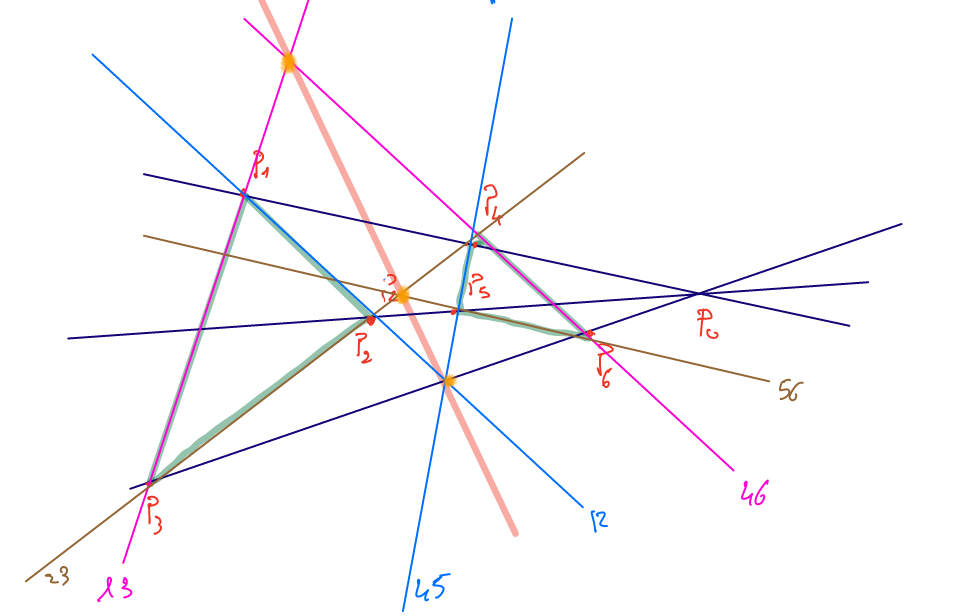
\includegraphics[scale=.35]{Desargues.png}
		\end{center}
	Siano $v_i\in V, \ \0\leq i \leq 6, $ t.c. $\ \ [v_i] = P_i$ Per ipotesi
	\[
	v_0 = \alpha_1v_1+\alpha_4v_4 = \alpha_2v_2+\alpha_5v_5=\alpha_3v_3+\alpha_6v_6
	.\] 
	Inoltre poiché $P_0\neq P_i, i > 1 ,$ tutti gli $\alpha_i$ sono non nulli.
	I punti \\
	\begin{aligend}
		&L(P_1,P_3)\cap L(P_4,P_6)\\
		&L(P_2,P_3)\cap L(P_5,P_6)\\
		&L(P_1,P_2)\cap L(P_4,P_5)
	\end{aligend} sono associati ai vettori \\
	\begin{aligend}		
&\alpha_1v_1-\alpha_3v_3=-\alpha_4v_4+\alpha_6v_6\\
&-\alpha_2v_2 + \alpha_3v_3=\alpha_5v_4-\alpha_6v_6 \\
&- \alpha_1v_1+\alpha_2v_2=\alpha_4v_4-\alpha_5v_5
		\end{aligend}\\
		I vettori nella colonna di sinistra sono dipendenti, poiché la loro somma è 0. Dunque i punti corrispondenti sono allineati.
	\end{dimo}
	\begin{teo}[Pappo]
	$A_1,\ldots,A_6$ distinti $L(A_1,A_2),L(A_2,A_3),\ldots,L(A_6,A_1)$ distinte\\
	esistono $r,s$ rette con $A_i\in r$, i dispari, $A_i\in s$ i pari\\
	Supponiamo poi $0=r\cap s\neq A_i.$ Allora 
	\[
	L(A_1,A_2)\cap L(A_4,A_5), \ \ L(A_2,A_3)\cap L(A_5,A_6),\ \ L(A_3,A_4)\cap L(A_6,A_1)
	.\] 
	sono allineati
\end{teo}
\begin{center}
	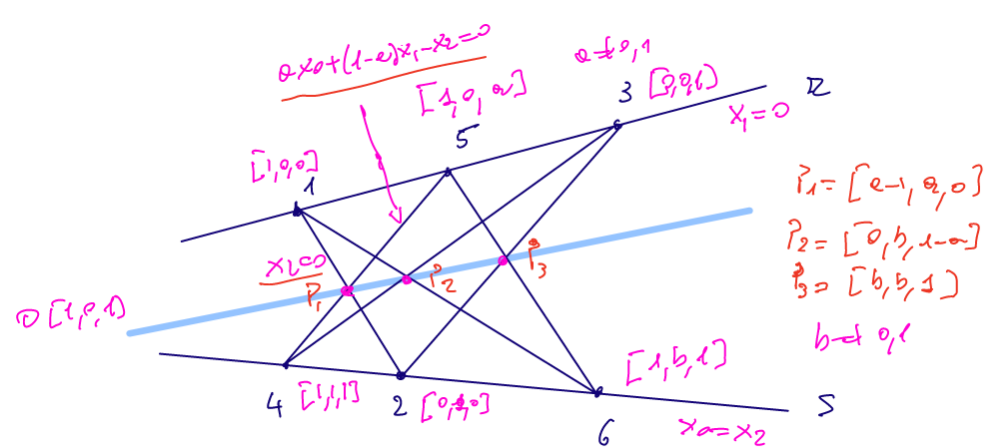
\includegraphics[scale=.45]{Pappo.png}
\end{center}
\begin{dimo}
	Poiché $r = L(A_1,A_3),\ \ s=L(A_2,A_4)$ sono distati e $0\neq A_i$\\
	$A_1,A_2,A_3,A_4$ è un riferimento proiettivo. Ma
	\[
		\det\matrice{a-1 & a & 0 \\ 0 &b &1 - a\\ b & b & 1} = 0 \Rightarrow  (a-1)b(1-1+a)+ab(1-a)=0
	\] 

\end{dimo}

\ \\ \hline \ \\
 $\pro=\pro(V)$ spazio proiettivo di dimensione $n$ $S = \pro (U),\ \ \ H = \pro(W)$ sottospazi proiettivi tali che 
 \[
  S\cap H = \emptyset \ \ \text{ e} \ \ \ L(S,H)=\pro
 .\] 
 Se $\dim S = k, \dim H = h$ per le formule di Grassmann
  \[
 k + h = n-1
 .\] 
$\forall P\in \pro\setminus H, \ \ \ \dim L(H,\{p\})=h+1$\\
Quindi $S\cap L(H,\{0\}) $ è un punto\\
Posso definire la proiezione su  $S$ di centro $H$ come
\[
 \pi^H_S: \pro\setminus H \rightarrow \pro
.\] 
\[
	P \rightarrow S\cap L(H,\{0\})
.\] 
$\pi^H_S$ è unna trasformazione proiettiva degenere indotta da $\pro^W_U :V \rightarrow V$ proiezione su $U$ parallela ad $H$\\
\begin{center}
	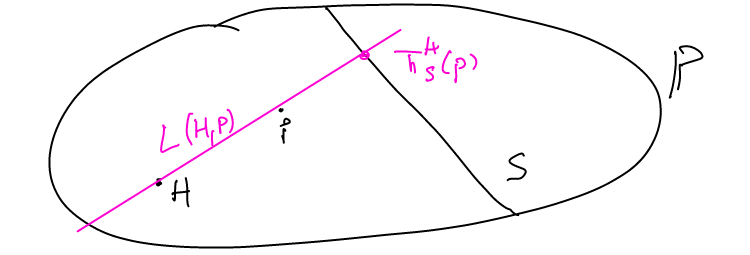
\includegraphics[scale=.45]{trasformazione_proiettiva.png}
\end{center}
\newpage
 \subsection{Proiettività}
 Siano in $\pro^2\ \ r,s$ rette distinte con $A = r\cap s$
  \begin{defi}
 	Dato $O\not\in r\cup s,$ la restrizione ad $r$ della proiezione su $s$ di centro $O$ è detta  \textbf{proiettività} di centro $O$
\end{defi}
\begin{center}
	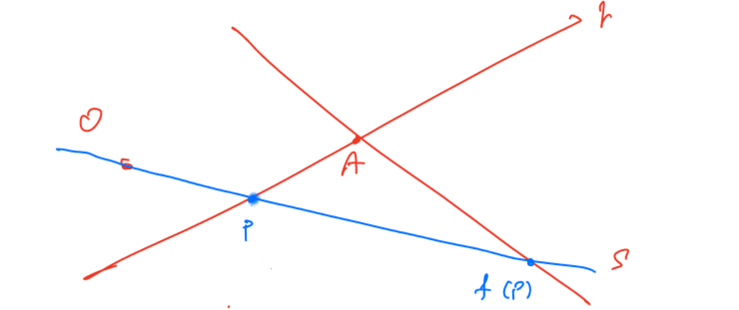
\includegraphics[scale=.6]{proiettivita.png}
\end{center}
$f$ è un isomorfismo proiettivo. La notazione si generalizza a $\pro^n$ nel modo seguente.\\
$S_1,S_2$ sottospazi di dimensione $k$, $H$ sottospazio tale che \[
H\cap S_1 = G\cap S_2 = \emptyset
.\] 
\[
\dim H = n  - k - 1
.\] Allora la restrizione a $S_1$ della proiezione su $S_2$ di centro $H$ è un isomorfismo proiettivo $f: S_1 \rightarrow S_2 $ detto prospettività di centro $H$
\newpage
\section{Curve algebriche}
\begin{defi}
	Una curva algebrica in $\A^2(K)$ è una classe di proporzionalità di polinomi non costanti di  $\K[x,y]$. Se  $f(x,y)$ è un rappresentante della classe, l'equazione 
	\[
	f(x,y) = 0
	.\] si dice equazione della curva
	\[
		\mathscr{C}= \{\icol{x\\y}\in \A^2|f(x,y) = 0\}
	.\] è il supporto della curva\\
	$\deg f$ grado della curva
\end{defi}
\begin{defi}
	Una curva algebrica di $\pro^2(\K)$ è una classe di proporzionalità di polinomi \underline{omogenei} di $\K[x_0,x_1,x_2]$. Se $F(x_0,x_1,x_2)$ è una rappresentazione della classe, l'equazione
	\[
	F(x_0,x_1,x_2)=0
	.\] 
	Si dice equazione della curva.\\ Le definizioni di grado e supporto sono analoghe a quelle affini
\end{defi}
\textbf{Caso affine}\\
Sia $T: \A^2 \rightarrow \A^2$ l'affinità $T(X) = AX + C$
 \[
	 A = (a_{ij})\in GL(2,\L) \ \ C = \matrice{c_1\\c_2}
.\] 
Sia $l$ una curva di equazioni $f(x,y) = 0$
La curva $D$ di equazione 
\[
g(x,y) =0 
.\] 
ove $g(x,y) = f(a_{11}x_1+a_{12}y+c_1,a_{21}x+a_{22}y+c_2)$ \\
è detta la trasformata di $l$ tramite $T^{-1}$
 \[
 D = T^{-1}(l)
.\] 
Se $T^{-1}X = BX + d$ \ \ $(B = A^{-1}, \ \ldots)$\\
allora  $g(b_{11}x + b_{12}y + d_1, b_{21}x+b_{22}y + d_2) = A(x,y)$\\
quindi $l = T(D)$\\
è chiaro che se  $p(x,y)\in D$ allora $T(p)\in l$ e viceversa.\\
quindi i supporti si dicono affinamente equivalente
\begin{defi}
	Data $\mathscr{C}$ curva affine, una curva affine $D$  si dice affinamente equivalente a $\mathscr{C}$ se esiste un'affinità $T$ tale che $\mathscr{C} = T(D)$
\end{defi}
\subsection{Ipersuperfici algebriche}
	Curva algebrica affine in $\A^2$ (proiettivo su $\pro^2$ ) La nozione si generalizza in modo ovvio al concetto di ipersuperficie (algebrica)
	\begin{defi}
		Una ipersuperficie algebrica in $\A^n$ (rispettivamente $\pro^n$ ) è una classe di proporzionalità di polinomi in
		\[
			\K[x_1,\ldots,x_n] \text{ (polinomi omogenei in } \K[X_0,\ldots,X_n])
		.\]
		($x$ sono coordinate affini, $X$ riferimento proiettivo)\\
		\begin{center}
			\begin{tabular}{c|c}
				
		$\underline{x} = (x_1,\ldots,x_n) \ \ & \underline X = (X_0,\ldots,X_n)$\\
		$\mathscr{C} = f(\underline x) = 0$ equazione della curva \ & $F(\underline X)=0$\\
		supporto di $\mathscr{C}\ \ \{\underline x\in\A^n|f(\unferline x)=0\}\ \ & \{ \left[X_0,\ldots,X_n\right]|F(\unferline X) =0 \}$ \\
		\varphi\in Aff(\A^n) \ \ \ \ &\psi \in PGL(n)\\
		$\mathscr{C} \text { ipersuperficie definita da } f(\underline x) = 0 & F(\underline X)\\
		\varphi(\mathscr{C}): \text{ ipersuperficie definita da } & \psi(\mathscr{C})\\
			f( \varphi^{-1}(\underline x))=0 & F(\psi^{-1}(\underline X)) = 0$
			\end{tabular}
		\end{center}
	\end{defi}
	$\mathscr{C} : x^2 + y^2 = 1 \ \ \ \ \varphi\matrice{x\\y} = \matrice{x+1\\y+1}\ \ \ \varphi^{-1}\matrice{x\\y}=\matrice{x-1\\y-1}$\\
	$ \varphi(\mathscr{C}): = (x-1)^2+(x-1)^2 = 1$ \ \ \ $\matrice{x\\y}:x^2 + y^2=1 \ \ \varphi\matrice{x\\u} $ ipersuperficie
	\begin{defi}
		Due ipersuperfici affini $\mathscr{C}_1,\mathscr{C}_2$(proiettivi) sono affinemente equivalenti (proiettivamente equivalenti), se esiste $ \varphi\in Aff(\A^n) (\psi \in PGL(n))
		\\$ 
		tale che $ \varphi(\mathscr{C}_1)=\mathscr{C}_2 (\psi(\mathscr{C}_1) = \mathscr{C}_2)$
	\end{defi}
	\textbf{Nota}:\\
	$x_1 = \frac {X_1} {X_0}$\\
	$f(\underline x) \rightarrow F(\underline X)$ e questo si chiama polinomio omogeneizzato di $F$ \\
	\textbf{Esempio}\\
$x + y + z - 3 = 0 \leadsto \ \ X_1+X_2+X_3-3X_0=0$\newpage
	\subsection {Chiusura proiettiva di $\mathscr{C}$ }
	La chiusura proiettiva dell'ipersuperficie affine di equazione $f(\underline x) =0$ è l'ipersuperficie proiettiva di equazione  $F(\underline X)=0$ dove  $F$ è il polinomio omogeneizzato  di $f$\\
	I punti di  $l^\star \cap H_0$ si chiama punti impropri di $\mathscr{C}$ ($\mathscr{C}^\star$ è la chiusura proiettiva)\\
	Se scriviamo $f$ come\\
	\[
	 f(\underline x) = f_0 + f_1(\underline x) + \ldots + f_n(\underline x)
	.\] 
	con gli $f_i$ omogenei di grado $i$
	 \[
		 F(X) = f_0 X_0^n + f_1(\underline X)X_0^{n-1}+\ldots+f_n(\underline X)
	.\] 
	ad esempio
	\[
	x^2 + 2xy + y^2 + z+ 2x-3 = 0
	.\] 
	diventa
	\[
	X_1^2 + 2X_1X_2 + X_2^2 +X_3X_0 + 2X_1X_0-3X_0^2=0
	.\] 
	punti impropri: intersecano con $X_0 =0 $\\
	\[
		[0,X_1,X_2,X_3]:X_1^2 + 2X_1X_2 + X_2^2 =0 
	.\] 
	Quindi l'equazione dei punti omogenei è data da 
	\[
	 f_n(\underline X) = 0
	.\] 
	\subsection{Classificazione delle coniche proiettive}
	Le coniche proiettive sono le curve di secondo grado in $\pro^2$\\
	:a generica equazione può scriversi 
	 \[
		 a_{11}X_1^2+2a_{12}X_1X_2+a_{12}X_2^2+2a_{01}X_0X_1+2a_{02}X_0X_2+a_{00}X_0^2
	.\] 
	Posto $a_{21}=a_{12}, a_{10}=a_{01},a_{20}=a_{02}$, la forma precedente si scrive come 
	\[
		(1)\ \ \ \ \ \ 	\underline X^t A X = 0 \ \ \ \ \ \text{ ove } A = (a_{ij})
	.\] 
	Se ora $M\in GL(3,\K)$ e rimpiazziamo $\underline X$ con $M\underline X$ da (1) si ottiene \\
	(2)\begin{aligend}
	&	(M\underline X^t)AM\underline X = 0\\
	&\underline X^t M A M \underline X =  0\\
	&\underline X ^t B \underline X = 0 \ \ \ \ B = M^t A M
	\end{aligend} \\
	Per definire $\mathscr{C}_2$ è proiettivamente a $\mathscr{C}_1$ \\
	Viceversa ogni conica poriettiva equivalente a $(\mathscr{C}_1)$ si ottiene in questo modo a partire da $M\in GL(3,\K)$ in definitiva\\
	classi di quivalenza proiettiva di coniche $\leftrightarrow $ classi di congruenza di matrici simmetriche 
	\newpage
	\begin{defi}
		La conica  $\underline X^tA\underline X = 0$ è:\\
		non degenere se  $\det A \neq 0$\\
		semplicemente degenere se  $rk A = 2$ e $\det A =0$\\
		doppiamente degenere se  $rk A  = 1$ e $\det A = 0$
	\end{defi}
	\begin{teo}
		Sia $\K$ algebricamente chisuo. Ogni conica di $\pro^2(\K)$ è proiettivamente equivalente a una delle seguenti\\
		$x_0^2+x_1^2+x_2^2 =0$ conica generale\\
		$x_0^2 +x_1^2 = 0$ conica semplicemente degenere\\
		$x_0^2=0$ conica doppiamente degenere\\
		Tali coniche non sono equivalenti tra loro
	\end{teo}
	\begin{dimo}
		Dobbiamo solo classificare le matrici simmetriche $3\times 3$ complesse rispetto alle componenti. Sappiamo che il rango è un invariante completo, quindi
		\[
			\matrice{1&0&0\\0&1&0\\0&0&1},\matrice{1&0&0\\0&1&0\\0&0&0},\matrice{1&0&0\\0&0&0\\0&0&0}
		.\] 
		sono le uniche possibilità.\\
	\end{dimo}
	\textbf{Nota:}\\
		Un invariante completo caratterizza la matrice (se hanno rango uguale allora sono equivalenti e viceversa)\\
	\begin{teo}
			Ogni conica di $\pro^2(\R)$ è proiettivamente equivalente a una delle seguenti:\\
			$x_0^2+x_1^2-x_2^2 =0 $ \ \ conica generale\\
			$x_0^2+x_1^2+x_2^2 =0 $ \ \ conica generale a punti non reali\\
			$x_0^2-x_1^2=0$ \\
			$x_0+x_1^2=0$ \ \ \ \ \ sono coniche semplicemente degeneri\\
			$x_0^2 =0$ \ \ \ \ \ \ \ \ \ \ conica doppiamente degenere
Queste coniche non sono equivalenti tra loro
	\end{teo}
	\newpage
	\begin{dimo}
		Utilizziamo il teorema di Sylvester per classificare le matrici reali simmetriche $3\times 3$ a meno di congruenza\\
		Sappiamo che gli indici sono invariante completo,\\
		ora ricordiamo che stiamo classificando polinomi omogenei a meno di proporzionalità\\
		\begin{center}
			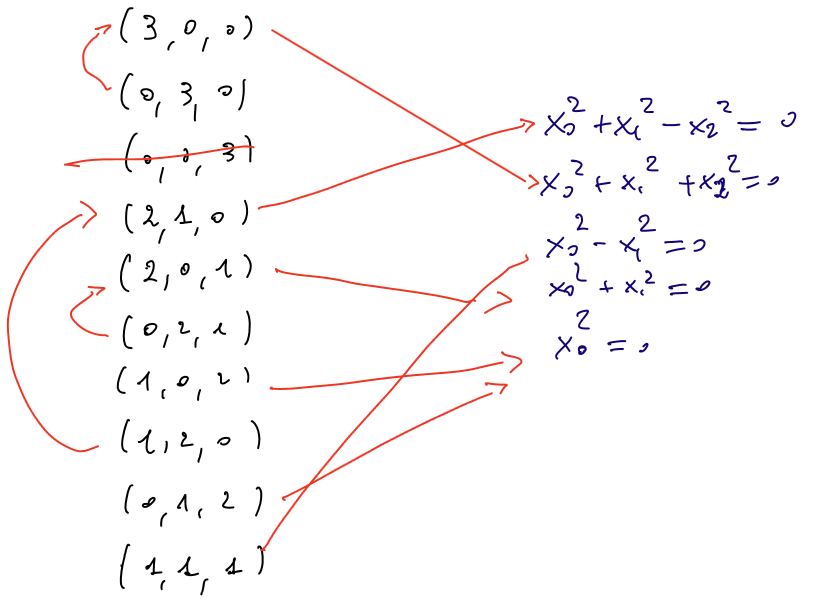
\includegraphics[scale=.4]{classificazione_coniche.png}
		\end{center}
		Quindi ogni conica proiettiva è equivalente a unna delle cinque elencate.\\
		Tali coniche non sono equivalenti perché hanno rango diverso oppure stesso rango ma supporti diversi
	\end{dimo}
	\textbf{Caso generale: quadriche proiettive}\\
	$\mathscr{C}: \ \ \ \ \underline X^t A \underline X =0 $ \ \ \  $A$ matrice simmetrica $(n+1)\times(n+1)$\\
	\newpage
	 \begin{teo}
		1.$\K$ algebricamente chiuso: ogni quadrica in $\pro^n(\K)$ è proiettivamente equivalente a una e una sola quadrica poichè
		\[
		 \sum^r_{i=1}x_i^2=0 \ \ \ \ 0\leq r\leq n
		.\] 
		2. $\K=\R$: ogni quadrica in $\pro^n(\R)$ è proiettivamente equivalente ad una e una sola quadrica
		\[
		\sum^p_{i=1}z_i^2 - \sum^r_{i=p+1}x_i^2=0
		.\] 
		$0\leq p \leq r\leq n, \ 2p\geq r-1, \ \ r\geq 1$
	\end{teo}
	\textbf{Esempio}\\
	$x_0^2 -1 x_1^2 + x_1x_2=0$\\
	 \[
		 A=\matrice{1&0&0\\0&1&1/2\\0&1/2&0}
	.\] 
	$\K=\C$ \ \ \ \ \ $\det A = -\frac 1 4\neq 0$ $\mathscr{C}$ è generale\\
	$\K = \R$\ \ \ \ \  $i_+\geq 1 \leadsto i_+=2,\ \ i_-=1,i_+=0$\\
	 $\leadsto $ equivalente a $x_0^2+x_1^2-x_2^2=0$
\subsection{Classificazione affine ed Euclidea}
	$\mathscr{C} \subset \A^2(\K) $ conica\\
	$\circledast a_{11}x^2 + a_{22}y^2 + 2a_{12}xy + 2a_{01}x + 2a_{01}y + a_{00}$\\
	pongo $a_{10}=a_{01}, a_{20}=a_{02},a_{21}=a_{12}$ dunque la matrice $A=(a_{ij})$ è simmetrica. Chiamo
	\[
		\widetilde{\underline X} = \matrice{1\\x\\y}. \text{ Allora } \circledast \text{ diventa}
	.\] 
	\[
	\underline{\widetilde{X}}^t A\underline{\widetilde{X}}
	.\] 
	Considera l'affinità $T_{M,C}(\underline X ) = M\underline X + c$ ove  $M\in GL(2,\K), \ \ b\in \K^2$\\
	Abbiamo visto che c'è un omomorfismo iniettivo 
	\[
	Aff(\A^2_\K) \rightarrow GL(3,\K)
	.\] 
	\[
		T_{M,C} \rightarrow \widetilde M = \matrice{ 1 & 0\ 0\\ c & M }
	\] 
	\[
		M = \matrice{m_{11}&m_{12}\\m_{21}&m_{22}} \ \ c = \matrice{c_1\\c_2}
	\] 
	Se effettuo il cambio di coordinate
	\[
		\widetilde{\underline{X}} = \widetilde{M}\widetilde{\underline{X}}'
	.\] 
	l'equivalenza $\widetilde{\underline{X}}^t A \widetilde{\underline{X}} = 0$ \\
	diventa  $(\widetilde M\widetilde{\underline{X}}')^t A \widetilde{M}\widetilde{\underline {X}}'$ \\
	\[
	\widetilde{\underline{X}}'^t B \widetilde{\underline{X}}'= 0
	.\] 
	con $B = \widetilde{M}^t A\widetilde{M}$\\
	Questa equazione ci dice che il rango di  $A$ è una proprietà affine di $\mathscr{C}$. Chiameremo tale numero rango di $\mathscr{C}$ (notazione $r(\mathscr{C})$\\
	Diciamo che  $\mathscr{C}$ è\\
	non degenere se $r(\mathscr{C}) = 3$\\
	semplicemente degenere se  $r(\mathscr{C}) = 2$\\
	doppiamente degenere se  $r(\mathscr{C}) = 1$
	\ \\ \hline \ \\
	$A = \matrice{a_{00}&a_{01} & a_{02}\\a_{01} & a_{11} & a_{12} \\ a_{02} & a_{12} & a_{22}}$ \\In altri termini, $A_0$ è la matrice della forma quadratica associata ai termini quadratici del polinomio $a_{11}x^2 + 2a_{12}xy + a_{22}y^ 2$ ($A_0$ è il minore ottenuto togliendo prima riga e prima colonna)\\
	\begin{aligend}
		& \widetilde{\underline{X}} = \widetilde M \widetilde{\underline{X}}'\\
		& A \leftrightarrow B = \widetilde M ^t A \widetilde M\\
		& A_0 \leftrightarrow B_0 = M^t A_0 M \circledast
	\end{aligend}\\
	Dunque anche $rk A_0$ è un invariante affine di $\mathscr{C}$ \\
	$\det A_0 \begin{cases}
		\neq 0 \ \ \ \mathscr{C} \text{ conica a centro }\\
		=0 \ \ \ \mathscr{C} \text{ parabola}
	\end{cases}$\\
	$\K = \R$ Da  $\circledast$ deduciamo che anche il segno di $\det A_0$ è un invariante affine (infatti $\det B = (\det M)^2 \det A_0)$\\
	\begin{center}
	 $\det B  \begin{cases}
		 >0 \ \ \mathscr{C} \text{ ellisse}\\
		 < 0 \ \ \mathscr{C} \text{ iperbole}
	 \end{cases}$
	\end{center}
	\newpage
	\begin{teo}
		Ogni conica di $\A^2(\K)$ è affinemente equivalente a una delle seguenti:\\
		1) $\K$ algebricamente chiuso \\
		$x^2 + y^2 - 1 = 0 \ \ $ conica a centro 1\\
		$x^2 + y^2 = 0 \ \ $ conica a centro degenere 2\\
		$y^2 -x = 0 \ \ $ parabola 3\\
		 $y^2-1=0$ \ \ \ parabola degenere 4\\
		 $y^2 = 0\ \ $ conica doppiamente degenere 5\\
		 2)  $\K = \R$\\
		  $x^2 + y^2 - 1 = 0$ \ \ ellisse 1\\
		  $x^2 + y^2 + 1 = 0$ \ \ ellisse a punti non reali 2\\
		  $x^2 + y^2 = 0$ \ \ ellisse degenere 3\\
		  $x^2 - y^2 -1 =0$ \ \ iperbole 4\\
		  $x^2 - y^2 = 0$ \ \ iperbole degenere 5\\
		  $y^2 - x =0 $ \ \ \ parabola 6\\
		  $y^2-1 = 0$ \ \ \ parabola degenere 7\\
		  $ y^2 + 1 = 0$ \ \ \ parabola degenere 8\\
		  $y^2 = 0$ \ \ \ conica doppiamente degenere 9 \\
 		  Le coniche di ognuno dei gruppi precedenti sono a due a due non affinemente equivalenti
	\end{teo}
	\begin{dimo}
		Partiamo da $\underline{\widetilde{X}}^t A X = 0$ e tramite affinità vogliamo ridurci ad uno dei casi elencati\\
		Passo 1:\\
		eliminazione del termine in xy \\ 
		Poichè $A_0$ è simmetrica, esiste $M\in GL(2,\K)$ tale che $M^t AM$ è diagonale. Quindi effetto la sostituzione $\underline X = M\underline X '$. L'equazione, nelle nuove coordinate $\underline X'$, che per comodità indichiamo ancora $\underline X$ è 
		\[
		a_{11}x^2 + a_{22}y^2 + 2a_{01}x + 2a_{02}y + a_00 = 0
		.\] 
		Osserviamo che la conica è a centro se e solo se $a_{11}a_{22}\neq 0$\\
		Passo 2\\
		Eliminazione dei termini lineari e costanti\\
		Supponiamo $\mathscr{C}$ a centro \\
		effettuiamo la traslazione $\begin{cases}
			x = x' - \frac {a_{01}}{a_{11}}\\
			y = y' - \frac{a_{02}}{a_{22}}
		\end{cases}$
		che cambia l'equazione in 
		$a_11 x'^2 + a_{22}y'^2 + c_00 = 0$\\
		Se $\mathscr{C}$ non è a centro possiamo supporre, a meno di scambiare le variabili (ovvero effettuare l'affinità $\matrice{0&1\\1&0}$) che risulti\\
		 \[
		a_11 =0, a_{22}\neq 0
		.\] \\
		$a_{22}y^2 + 2a_{01}x + 2a_{02}y + a_{00} =0 $\\
		Tramite la traslazione $ \begin{cases}
			x = x'\\
			y = y'-\frac {a_{02}}{a_{22}}
		\end{cases}$ \\
		l'equazione diventa
		\[
		a_22y^2' + 2a_{01}x' + d_{00}=0
		.\] 
		Se $a_{01}\neq 0$ eseguo $ \begin{cases}
			x' = x'' - \frac {d_{00}}{2a_{01}}\\
			y' = y''
		\end{cases}$\\
		ottenendo $a_{22} y''^2 + 2 a_{01}x''=0$\\
		se $a_{01} = 0$ \  \ $a_{22} y'^2 + d_{00}=0$\\
		Passo 3\\
		Normalizzazione dei coefficienti \\
		$\K = \overline \K$. Sia  $\mathscr{C}$ a centro. Partiamo da 
		\[
		 a_{11}x'^2 + a_{22}y'^2 + c_{00} =0
		.\] 
		se $c_{00} = 0 \ \ \begin{cases}
			x' = \frac {x} {\sqrt {a_{11}}}\\
			y'  = \frac y {\sqrt{a_{22}}}
		\end{cases} \leadsto \ \ x^2 + y^2 = 0 \ \ (2)$ \\
		Se $c_{00} \neq 0$
		\[
			-\frac {a_{11}}{c_{00}}x^2 ' - \frac{a_{12}}{c_{00}}y^2 ' - 1 = 0
		.\] 
		\[
		 \begin{cases}
			 x' = \sqrt{-\frac {c_{00}}{a_{11}}}x\\
			 y'= \sqrt{-\frac{c_{00}}{a_{22}}}y
		 \end{cases} \leadsto x^2 + y^2 -1 = 0(1)
		.\] 
		Sia ora $\mathscr{C}$ non a centro, trasformata in 
		\[
		 a_{22} y^2 ' + d_{00} = 0
		.\] 
		$d_{00} =0  \ \ \ \ y^2 ' =0 \leadsto \ \ y^2 =0 (5)$\\
	$d_{00}\neq 0 \ \ \ \ -\frac {a_{22}}{d_{00}}y^2' \ - 1 =0 $
	\[
	 \begin{cases}
		 y'= \sqrt{-\frac{d_{00}}{a_{22}}}y\\
		 x' = x
	 \end{cases} \leadsto y^2 - 1 = 0 (4)
	.\]
	Resta da vedere il caso $\mathscr{C} $ non a centro trasformata in 
	\[
	 a_{22} y'´ ^2 + 2a_{01}x''= 0
	.\] 
	\[
	 \begin{cases}
		 x''= \frac x {-2a_{01}}\\
		 y'' = \frac y {\sqrt{a_{22}}}
	 \end{cases}\leadsto y^2-x = 0 (3)
	.\] \\
	$\K = \R \ \ \mathscr{C} $  a centro\\
	\[
	 a_{11} x'^2 + a_{22}y^2 ' + c_{00} =0 
	.\] 
	Posso supporre $c_00 =0 $ o $c_00 = -1$\\
	\[
	 \begin{cases}
		 x'= \frac x {\sqrt{|a_{11}|}}\\
		 y' = \frac y {\sqrt{|a_{22}|}}
	 \end{cases}\leadsto (1)-(5)
	.\] 
	$\mathscr{C}$ non a centro del tipo
	\[
	a_{22}y'^2 + d_00 = 0
	.\] 
	Posso supporre $d_{00} = 0$ o $d_{00} = -1$\\
	\[
	\begin{cases}
		x' = x\\
		y' = \frac y {\sqrt{|a_{22}|}}
	\end{cases} \leadsto (7) - (9)
	.\] \\
	$\mathscr{C} $a centro del tipo 
	\[
		a_{22} y''^2 + 2a_{01}x'' = 0
	.\] 
	Posso supporre $a_{22} >0$ e effettuare $ \begin{cases}
		x'' = \frac x {-2 a_{01}}\\
		y'' = \frac y {\sqrt{a_{22}}}
	\end{cases}$ \leadsto 6
	\end{dimo}
	\textbf{Osservazioni}\\
	1) Se $\mathscr{C}$ è a centro, il sistema lineare
	\[
	\begin{cases}
		a_{11}x + a_{12}y + a_{10} = 0\\
		a_{22}x + a_{22}y + a_{20} = 0
	\end{cases}
	.\] 
	Ha soluzione unica (poiché $\det A_0 \neq 0)   \ \ (x_0,y_0) $\\
	Il punto con tali coordinate è il centro di simmetria, infatti la simmetria rispetto a tale punto 
	\[
	 \begin{cases}
	 	x = 2x_0-x'\\
		y = 2y_0-y'
	 \end{cases}
	.\] 
	manda $\mathscr{C}$ in $\mathscr{C}$\\
	Le rette passanti per $c = \matrice{x_0\\y_0}$ si dicono diametri di $\mathscr{C}$\\
	2) per calcolare i punti impropri di $\mathscr{C}$ di equazione
	\[
		\underline{\widetilde{X}}^tA\underline{\widetilde{X}} = 0
	.\] 
	bisogna risolvere l'equazione omogenea
	\[
		a_{11}x_1^2 + 2a_{12}x_1x_2+a_{22}x_2^2 = 0
	.\] 
	$\displaystyle \left(x = \frac {x_1}{x_0}, \ \ y = \frac{x_2}{x_0}\right)$ che ha discriminante $-det A_0$. Quindi le soluzioni sono\\
	reali distinte $\mathscr{C}$ iperbole\\
	reali coincidenti $\mathscr{C}$ parabola\\
	complesse coniugate $\mathscr{C} $ ellisse
	\begin{teo}
		Ogni conica di $\mathbb{E}^2$ è congruente a una delle seguenti\\
		\begin{aligned}
			&\frac{x^2}{a^2} + \frac {y^2}{b^2} = 1 \ \ a\geq b> 0 \ \ \text{ ellisse}\\
			&\frac{x^2}{a^2} + \frac {y^2}{b^2} = -1 \ \ a\geq b > 0 \text{ ellisse a putni non reali}\\
			&\frac{x^2}{a^2} + \frac {y^2}{b^2} = 0 \ \ a\geq b > 0 \text{ ellisse degenere}\\
			&\frac{x^2}{a^2} - \frac {y^2}{b^2} = 1 \ \ a>0, b > 0 \text{ iperbole}\\
			&\frac{x^2}{a^2} - \frac {y^2}{b^2} = 0 \ \ a>0, b > 0 \text{ iperbole degenere}\\
			&y^2 - 2px = 0 \ \ p>0\text{ parabola}\\
			&y^2 - a^2 = 0 \ \ a\geq0\text{ parabola degenere}\\
			&y^2 + a^2 = 0 \ \ a>0\text{ parabola degenere}\\
			&y^2 =0 \ \ \text{ conica doppiamente degenere}
		\end{aligned}
		\\
		le coniche elencate sono a due a due non equivalenti
	\end{teo}

	\textbf{Osservazioni}\\
	1. Metrico $=$ euclideo\\
	2. Per distinguere l'ellisse non degenere a punti reali da quella a punti immaginari, si può usare il seguente criterio
	\[
		A=(a_{ij})^2_{i,j=0} \ \ A_0=(a_{ij})^2_{i,j=1}
	.\] 
	$tr A_0 \det A $ \begin{cases}
		>0 \text{ellisse a punti immaginari}\\
		<0 \text{ellisse a punti reali}
	\end{cases}\\
$ \displaystyle\lambda_1 x^2 + \lambda_2 y^2 + \frac{\det A}{\det A_0} = 0$\\
Non ci sono soluzioni reali se e solo se $\lambda_1 ($ o  $\lambda_2)$ hanno lo stesso segno di $\det A$, è equivalente dire
\[
tr A_0 \det A >0
.\] 
\subsection{Geometria delle coniche euclidee}
\textbf{Ellissi}\\
$\displaystyle \frac{x^2}{a^2} + \frac {y^2}{b^2}=1 \ \ \ \ \ a\geq b>0$\\
 $a = b \ \ \ x^2 + y^2 = a^2$ circonferenza di centro l'origine e rango $a$ \\
 Il  supporto dell'ellisse è chiuso e limitato, infatti esso è centrato nel rettangolo delimitato dalle rette $x\pm a, \ \ y=\pm b$
  \[
	  supp \ \ \mathscr{C} \subset \{ (x,y)\in\R^2 : |x|\leq a , \ |y| \leq b\}
 .\] 
\begin{center}
	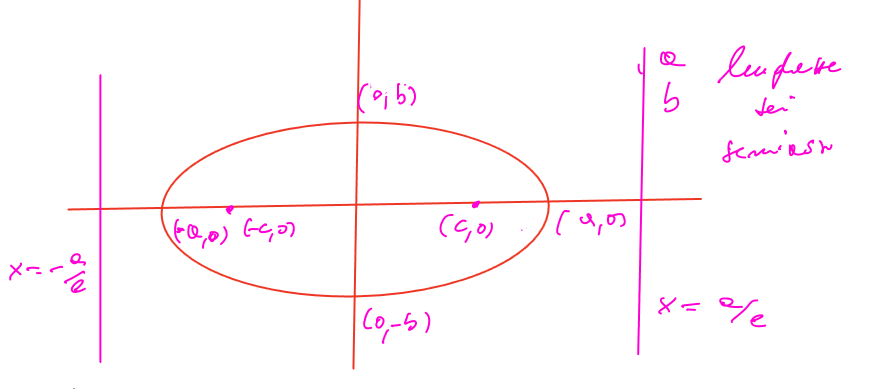
\includegraphics[scale=.45]{ellisse.png}
\end{center}
  $\displaystyle\frac {x^2}{a^2} + \frac{y^2}{b^2} \leadsto y=\frac b a \sqrt{a^2-x^2}, \ \ y = =\frac b a \sqrt{a^2-x^2}$ \\
  \begin{defi}
	  $c = \sqrt{a^2-b^2} \ \ (\pm c, 0) $ fuori di $\mathscr{C}$
	   \[
		   e = \frac c a \ \ \ \text{eccentriche di }\mathscr{C}
	  .\] 
  \end{defi}
  \textbf{Nota}\\
  $0 \leq e < 1, \ \ e = 0 \Leftrightarrow\mathscr{C}$ circonferenza
  \[
	  x =\pm \frac a c  \text{direttrici di \mathscr{C}}
  .\] 
  + rispetto a $(c,0)$, - rispetto a  $(-c,0)$\\
  \textbf{Iperbole}\\
  $\displaystyle\frac {x^2}{e^2} - \frac{y^2}{b^2} = 1 \ \ a > 0, b > 0$\\
\begin{center}
	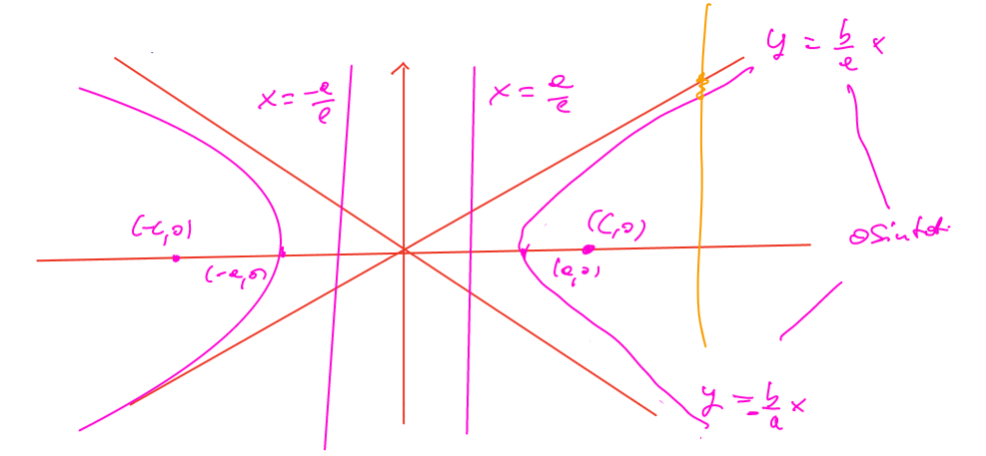
\includegraphics[scale=.45]{iperbole.png}
\end{center}
  \begin{defi}
	  $c = \sqrt{a^2 + b^2} \ \ (\pm c,0)$ fuochi di $\mathscr{C}$ 
	   \[
		   e = \frac c a \ \ \ \ \text{eccentricità } e>1
	  .\] 
	  \[
		  x = \pm \frac a c \ \ \text{ direttrici}
	  .\] 
  \end{defi}
  \textbf{Parabola}\\
  $y^2 = 2 px \ \ p>0\ \ \ y = \pm\sqrt{2px}$\\
\begin{center}
	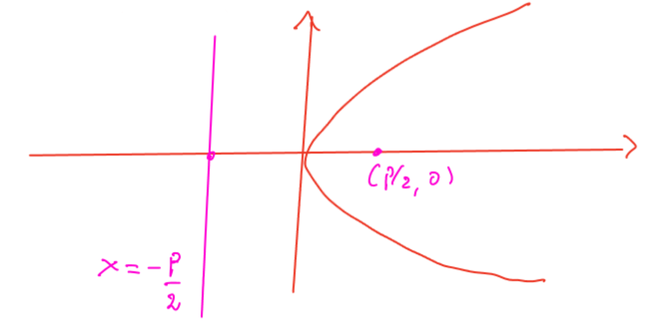
\includegraphics[scale=.45]{parabola.png}
\end{center}
\begin{defi}
	Il fuoco di $\mathscr{C}$ \ \ \ $(\frac p 2 , 0)$
	 \[
		 \text{ direttrice } \ \ x = -\frac  p 2 \ \ \ e = 1 \ \ \text{eccentricità}
	.\] 
\end{defi}
\begin{prop}
	L'ellisse (1) e l'iperbole (2) hanno per supporto il luogo dei punti le cui distanze dai due fuochi ha somma (rispettivamente differenza) costante (rispettivamente costante in valore assoluto) uguale a $2a$
\end{prop}
\begin{prop}
	L'ellisse (1), l'iperbole (2), la parabola (3) hanno per supporto il luogo dei punti le cui distanze da un fuoco e dalla relativa direttrice hanno rapporto costante uguale ad $e$ l'eccentricità della conica
\end{prop}
\begin{dimo}[proposizione 1]
	Siano $F, F'$ i fuochi, di coordinate $(c,0),(-c,0)$ rispettivamente.
	Imponiamo la condizione
	\[
	|d(P,F)\pm d(P,F')| = 2a
	.\] 
	Se $P$ ha  coordinate $(x,y)$ risulta \[
		|\sqrt{(x-c)^2+y^2}\pm\sqrt{(x+c)^2 + y^2}| = 2a \ \ \cirlcedast\circledast
	.\] 
	Elevando due volte al quadrato, otteniamo 
	\[
		\frac{x^2}{a^2} + \frac{y^2}{a^2-c^2} = 1 \ \ \cirlcedast
	.\] 
	Se $c = \sqrt{a^2 - b^2} \leadsto \frac{x^2}{a^2} + \frac{y^2}{b^2} =1$ ellisse\\
	Se $c = \sqrt{a^2 + b^2} \leadsto \frac{x^2}{a^2} - \frac {y^2}{b^2} = 1$ iperbole\\
	Per concludere, osserviamo che il luogo rappresentato da $\circledast$ è precisamente (1) nel caso dell'ellisse e (2) nel caso dell'iperbole\\
	A questo scopo, basta osservare che il procedimento è reversibile a meno di affinità di segni nei radicali. Però la conclusione\\
	\[
		c < a \ \ \text{ è compatibile col prendere} + \text{nell'equazione} \circledast\circledast
	.\] 
	\[
		c > a \ \ \text{ è compatibile col prendere} - \text{nell'equazione} \circledast\circledast
	.\] 
\end{dimo}
\begin{dimo}[proposizione 2]
	La condizione che definisce il luogo cercato è 
	\[
		\frac{d(P,F)}{d(P,r)}=e
	.\] 
	$ P = (x,y)$
	\begin{tikzpicture}[remember picture, overlay]
		\node[xshift=120mm,yshift=-122mm,anchor=north west] at (current page.north west){%
		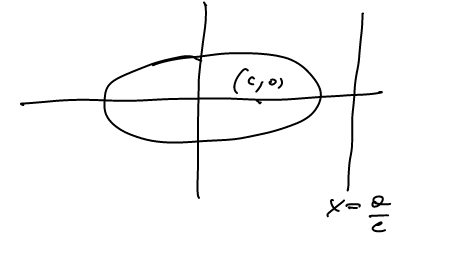
\includegraphics[width=40mm]{ellisse_prop.png}}
	\end{tikzpicture}
	 \[
		 \frac{\sqrt{(x-c)^2+y^2}}{|x-\frac{a}{c}|}=e
	.\] 
	$(x-c)^2 + y^2 = e^2 (x-\frac a e)^2$ \\
	$x^2 - 2cx + c^2 + y^2 = e^2x^2 - 2aex + a^2$\\
	$x^2 (1-e^2) + y^2 = \cancel{2(c - ea)x} + a^2 - c^2$ dato che $c = \frac e a$ e  $e = \frac c a$\\\
	$(1 - \frac {c^2}{a^2})x^2 + y^2 = b^2$ \\
	$\frac{a^2 - c^2}{a^2}x^2 + y^2 = b^2$\\
	$\frac{b^2}{e^2}x^2 + y^2 = b^2$\\
	$\frac{x^2}{a^2} + \frac{y^2}{b^2} = 1$\\
	Gli altri cambi per l'iperbole sono analoghi e lasciati per esercizio
\end{dimo}
\newpage
\begin{center}
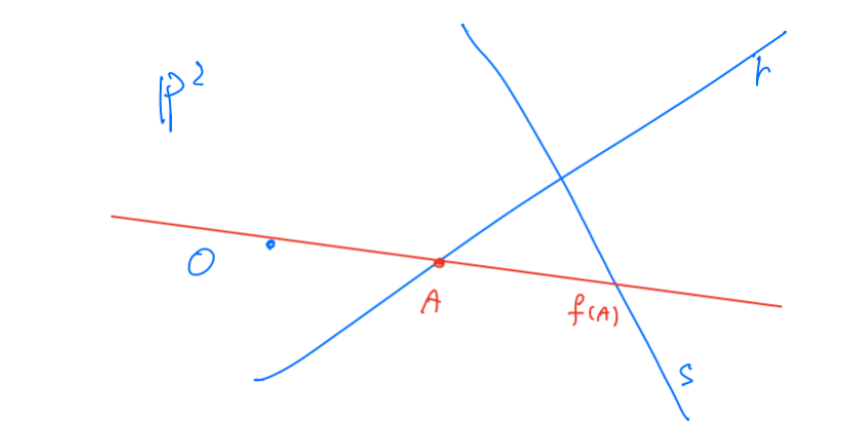
\includegraphics[scale=.4]{prospettivita_2.png}
\end{center}
Più in generale, dati $S_1,S_2$ spazi proiettivi tali che $\dim S_1 = \dim S_2 = k$ in $\pro^n$, e  $H$ sottospazio $H\cap S_1 = H\cap S_2 =\emptyset$ e $\dim H = n - k -1 $, la prospettività di centro $M$ è la restrizione a $S_1$ della proiezione su $S_2$ di centro $H$ ; è un isomorfismo $S_1 \rightarrow S_2$\\
\textbf{Esercizio}\\
Siano in $\pro^3$ $T_1$ il piano $x_3 = 0$ e $T_2$ il piano $x_0+2x_1-3x_2=0$\\
\[
	Q = [0,1,-1,1], \ \ f: T_1 \rightarrow T_2 \ \ \text{ di centro } Q
.\] 
Trova equazioni cartesiane dell'immagine di $r=T_1\cap T_3$ dove $T_3:x_0+x_1=0$\\
Risulta $f(r) = L(Q,r)\cap T_2$\\
$r$ ha equazioni  \begin{cases}
	x_3=0\\
	x_0+x_1=0
\end{cases}\\
Il fascio di piani di asse $r$ ha equazione
\[
	\lambda(x_0+x_1)+\mu x_3=0 \ \ \ \ \ [\lambda,\mu]\in\pro^1(\R)
.\]
Imponendo il passaggio per $[0,1,-1,1]$ otteniamo\\
\[
	\lambda + \mu =0 \ \ \ \ [\lambda,\mu] = [1,-1]
.\] 
$L(Q,r):x_0+x_1-x_3=0 \ \ f(r) \ \  \begin{cases}
	x_0+x_1-x_3=0\\
	x_0+2x_1-3x_2
\end{cases}$
\ \\ \hline\ \\ 
Siano $r,s\subseteq\pro^2(\R)$ rette distinte, $A=r\cap s$ e $f:r \rightarrow s$ un isomorfismo proiettivo allora.\\
(a) $f$ è una prospettività se e solo se $f(A) = A$\\
(b) Se  $f(A)\neq A , $ esiste una retta $t$ in $\pro^2$ e due prospettività $g: r \rightarrow t, \ \ h : t \rightarrow s$ tale che
\[
 f = h\circ g
.\] 
(c) Ogni proiettività $p:r \rightarrow r$ è composizione di al più tre prospettività
\\
$(a)$ per costruzione una prospettività fissa il punto $A$\\
\begin{center}
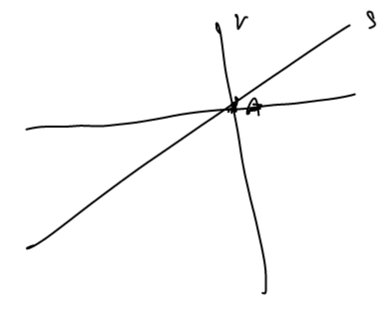
\includegraphics[scale=.5]{prospettivita_3.png}
\end{center}
 Viceversa, supponiamo che $f:r \rightarrow s$ sia tale che $f(A) = A$ 
\begin{center}
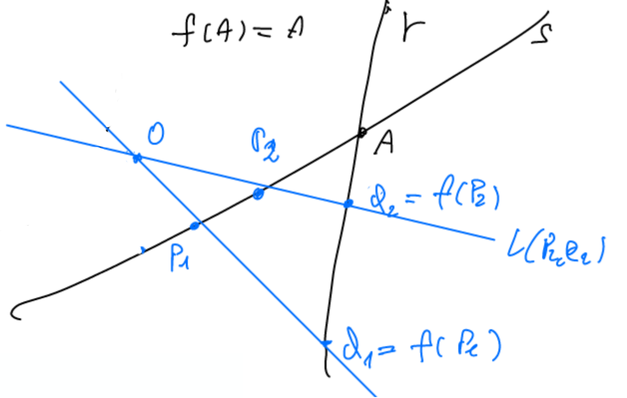
\includegraphics[scale=.5]{prospettivita_4.png}
\end{center}
 $L(P_1,Q_1)\cap L(P_2,Q_2) = 0 \not \in r\cup s$\\
 Se $g$ è la prospettività di centro $O$, risulta $g(A) = A,\ \  g(P_1)=Q_1, \ \ g(P_2)=Q_2$\\
 Ma $A,P_1,P_2, \ \ \ A,Q_1,Q_2$ sono punti in posizione generale\\
 e pertanto, per il teorema fondamentale, $f=g$
 \newpage
 \begin{nome}
 	Classificazione metrica delle quadriche  non degeneri in $\R^3$
	\begin{center}
		
	\begin{tabular}{ c c c }
		$\frac{x^2}{a^2} + \frac{y^2}{b^2} + \frac{z^2}{c^2}=1$ &$ a > b > c > 0$ & $\text{ ellissoide}$ \\ 
		$\frac{x^2}{a^2} + \frac{y^2}{b^2} - \frac{z^2}{c^2}=1$ &$ a > b >0, c > 0$ & $\text{ iperboloide iperbolico} $\\
		$\frac{x^2}{a^2} - \frac{y^2}{b^2} - \frac{z^2}{c^2}=1$ &$ a > 0,b > c > 0$ & $\text{ iperboloide ellittico} $\\ 
		$\frac{x^2}{a^2} + \frac{y^2}{b^2} - z = 0$ &$ a > b > 0$ & $\text{ paraboloide ellittico} $\\ 
		$\frac{x^2}{a^2} - \frac{y^2}{b^2} - z=0$ &$ a, b > 0$ & $\text{ paraboloide iperbolico} $\\ 
	\end{tabular}
	\end{center}
 \end{nome}
 \begin{teo}
 	1) L'applicazione 
	\[
		\pro\setminus H\times\pro\setminus H \rightarrow Hom_{\K}(V\setminus H, H)
	.\] 
	\[
		(p,p') \ \ \ \rightarrow \ \ \ \varphi_{p,p'}
	.\] 
	definisce su $\pro\setminus H$ una struttura di spazio affine con spazio vettoriale associato $Hom_{\K}(V\setminus H, H)$.\\
	Inoltre, per ogni spazio proiettivo $S = \pro(W)$ di $\pro$ non contenuto in  $H$, $S\cap \pro\setminus H$ è un sottospazio affine di $\pro\setminus H$ con giacitura
	\[
	Hom(V\setminus H, W\cap H)
	.\] 
	2) Dato nello spazio vettoriale $V$ (pensato come spazio affine) un iperpiano affine $A$ di giacitura $H$, non contentente $O$, si definisce su $\pro\setminus H$ una struttura di spazio affine con spazio vettoriale associato $H$ tramite
	\[
	\pro\setminus H\times\pro\setminus H \rightarrow H
	.\] 
	\[
		(p,p') \ \ \ \rightarrow \ \ \ a'-a
	.\] 
	\[
	a = A\cap <u>, \ \ a' = A\cap <u'>
	.\] 
 \end{teo}
 Di quest'ultimo teorema, il papi non ci lascia la dimostrazioni, ma solo eterna frustrazione nelle nostre povere vite.
\end{document}
